\documentclass[article,type=msc,colorback,accentcolor=tud9c]{tudthesis}
\usepackage{ngerman}
\usepackage[american,ngerman]{babel}
\usepackage{tabularx} % better tables
\usepackage{colortbl}
\usepackage[hyphens]{url}
\usepackage[ngerman]{hyperref}	% urls
\usepackage{enumitem}
\usepackage{listings}	% nicer lists
%setup special characters in listing
\lstset{literate=
  {á}{{\'a}}1 {é}{{\'e}}1 {í}{{\'i}}1 {ó}{{\'o}}1 {ú}{{\'u}}1 {ù}{{\`u}}1
  {Á}{{\'A}}1 {É}{{\'E}}1 {Í}{{\'I}}1 {Ó}{{\'O}}1 {Ú}{{\'U}}1
  {à}{{\`a}}1 {è}{{\'e}}1 {ì}{{\`i}}1 {ò}{{\`o}}1 {ò}{{\`o}}1
  {À}{{\`A}}1 {È}{{\'E}}1 {Ì}{{\`I}}1 {Ò}{{\`O}}1 {Ò}{{\`O}}1
  {ä}{{\"a}}1 {ë}{{\"e}}1 {ï}{{\"i}}1 {ö}{{\"o}}1 {ü}{{\"u}}1
  {Ä}{{\"A}}1 {Ë}{{\"E}}1 {Ï}{{\"I}}1 {Ö}{{\"O}}1 {Ü}{{\"U}}1
  {â}{{\^a}}1 {ê}{{\^e}}1 {î}{{\^i}}1 {ô}{{\^o}}1 {û}{{\^u}}1
  {Â}{{\^A}}1 {Ê}{{\^E}}1 {Î}{{\^I}}1 {Ô}{{\^O}}1 {Û}{{\^U}}1
  {œ}{{\oe}}1 {Œ}{{\OE}}1 {æ}{{\ae}}1 {Æ}{{\AE}}1 {ß}{{\ss}}1
  {ç}{{\c c}}1 {Ç}{{\c C}}1 {ø}{{\o}}1 {å}{{\r a}}1 {Å}{{\r A}}1
  {€}{{\EUR}}1 {£}{{\pounds}}1
}
\lstset{breaklines=true}
\lstset{numbers=left}
\lstset{tabsize=2}
\usepackage{cleveref}
\usepackage{lineno}
\usepackage{color, colortbl}
\usepackage{longtable}
\usepackage{subfigure}

\newcounter{dummy} % necessary for correct hyperlinks (to index, bib, etc.)

\linespread{1.2}\selectfont

\newcommand{\getmydate}{%
  \ifcase\month%
    \or Januar\or Februar\or M\"arz%
    \or April\or Mai\or Juni\or Juli%
    \or August\or September\or Oktober%
    \or November\or Dezember%
  \fi\ \number\year%
}

%\definecolor{rowColorHead}{rgb}{0.7,0.7,0.7}
%\definecolor{rowColor1}{rgb}{0.9,0.9,0.9}
%\definecolor{rowColor2}{rgb}{255,255,255}

\hypersetup{%
  pdftitle={Design, implementation and evaluation of an anti-phishing app},
  pdfauthor={Clemens Bergmann und Gamze Canova},
  pdfview=FitH,
  pdfstartview=FitV
}

\setinstitutionlogo[height]{graphix/secuso.jpg}

\begin{document}
\selectlanguage{american}
  \thesistitle{Design, Implementation and Evaluation of an Anti-Phishing Education App}{Design, Implementatierung und Evaluierung einer Anti-Phishing Education App}
  \author{Clemens Bergmann und Gamze Canova}
  %\birthplace{Darmstadt}
  \referee{Professor Dr. Melanie Volkamer}{Arne Renkema-Padmos}
  \department{Fachbereich Informatik}
  \group{Security, Usability and Society}
  %\tuprints{12345}{1234}
  %TODO:tuprints klären
  \makethesistitle
  \affidavit{C. Bergmann}
  \affidavit{G. Canova}

 \tableofcontents

	%======================================================
	% CONTENT
	%======================================================
	\cleardoublepage
	\pagenumbering{arabic}
	
	
	% !!!!!!!!!!! WOERTER VEREINHEITLICHEN: !!!!!!!!!!!
	%anti-phishing
	%capitalization
	%website / web site
	%email / e-mail
	%...
	% pre-study/prestudy mit phishing survey ersetzen!!!
	%	\linenumbers

	%Abstract:
	\selectlanguage{ngerman}
\begin{abstract}
%TODO:Deutschen Abstract anpassen. Siehe englischer abstract
Immer mehr Betrüger entdecken das Internet als Platz ihres Handelns. Dazu
versenden sie gefälschte Emails oder veröffentlichen gefälschte Webseiten, die
den Benutzer auffordern private Daten einzugeben. Dieses Vorgehen nennt man
Phishing. Dieses kann für die Opfer sowohl wirtschaftliche als auch private
Folgen haben. Neben technischen Verbesserungen ist auch eine ausreichende
Schulung der Benutzer über die Gefahren und Risiken im Internet ein wichtiger
Bestandteil einer Strategie gegen Phishing.
Unsere Master-Arbeit hat zum Ziel eine Smartphone-Anwe<wbr>ndung zu entwickeln, die
dem Benutzer Hilfestellungen an die Hand gibt, um in Zukunft seltener Opfer von
zu werden. Dazu macht sie den Benutzer mit Methoden der Angreifer
bekannt und hilft ihm durch Üben diese zu verinnerlichen.
\end{abstract}

\selectlanguage{american}
\begin{abstract}
Scammers discover the Internet as a convenient place for their criminal activities. 
For instance, they send Internet users spoofed e-mails or publish fraudulent websites which prompt users to enter their confidential data. 
This kind of Internet fraud is referred to as phishing. 
For a victim of a phishing attack the consequences can be of an economic as well as an emotional nature. 
There exist multiple technical solutions to approach the problem of phishing. 
Yet, they all cannot guarantee 100\% accuracy.
Moreover, sometimes security warnings or indicators of such approaches are ignored by end users.
For this reason a complementary approach is required.
We believe that the increase of security awareness and especially user education about the dangers of the Internet, is a further key strategy to combat phishing. 
Our master thesis aims at developing a smartphone app, which increases security awareness and educates the user regarding phishing.
To increase security awareness the users send themselves a spoofed e-mail right away when starting the app for the first time.
This shall exemplary illustrate them how trivial e-mail spoofing is and is intended to increase their motivation and engagement ultimately leading to better knowledge retention.
The user education part entails alerts regarding known techniques of attackers and helps them to internalize these by practice and repetition.
In detail, our app is realized as a quiz based game which mainly focuses on the detection of phishing URLs.
Ultimately, the app should enable the users to achieve the capability of defending themselves against phishing attacks in the future, in case technical solutions should fail.
In order to evaluate the effectiveness of the app a user study is conducted.
The study outcomes shows that our app in general receives positive feedback from the users and also helps them make better decisions on whether a given URL is legitimate or fraudulent.
\end{abstract}


	%*******************************************
%*******************************************
\section{Introduction}
%*******************************************
\label{s:introduction}
%subject
This chapter introduces the target of this work, which is to design, implement and evaluate an educational app.
 The app is supposed to help unexperienced users detect phishing attacks.
 At first we motivate the benefit of our work and how we envision our approach to achieve our goal.
Specifically, we first motivate why countering phishing is necessary by exploring the consequences and statistics of phishing.
Subsequently, we will reason why there is a need for an anti-phishing education app, instead of, for example, a further technical solution or a computer-based educational approach.
 Finally, we define our specific objectives and provide an overview of the following chapters.


%===========================================
\subsection{Motivation}
%===========================================
Nowadays, a world without Internet is unimaginable for most people in developed countries.
As an example, 83\% of Germany's population have Internet access~\cite{globalfinance2012internetusage}. 
However, it is undeniable that with the benefits of the Internet also come threats. 
One major issue of today's digitalized world is phishing. 

Phishing is a form of fraud to lure confidential information from users, cf. \autoref{s:phishing_def}. The goal of the attacker is to impersonate the user in online systems.
 This can be used to access corporate systems, damage the users reputation or simply steal money from him.
 Usually, phishing happens through fake websites which imitate the original ones.
 On these so called phishing websites the users are asked to enter confidential data, such as their login or bank account data.
 In this section we elaborate on the importance of countering such phishing attacks with the aid of user education. 



%-------------------------------------------
\subsubsection{Consequences of Phishing}
%-------------------------------------------
Falling for a phishing attack has several consequences for the fooled person as well as for the target company or organization.
 In the following some of these consequences are briefly illustrated.

\begin{description}[leftmargin=0cm]
	\item[Identity and Data Theft] Phishing is the practice of tricking users to disclose their personal data.
 That is to say, a possible consequence of falling for a phishing attack is identity theft~\cite{jakobsson2006phishing}.
 With the data unknowingly provided by the victims, the attacker can impersonate them on their behalf.
 For example, he can do online shopping or transfer money to his account on behalf of his victims.
 In a corporate scenario the attacker might even gain access to secured systems by attacking an administrator.
 When the attacker has access to these systems he might be able to collect customer data.
 Therefore not only users who are subject to phishing attacks can be affected by the attack, but also the institutions, organizations, companies and also their customers.
	\item[Financial Loss] Financial loss can be the result of users' banking accounts being plundered or increased support costs for the targeted institutions due to their customers who fell for an attack~\cite{rsa2013, mcafee}.
	\item[Reputational Damage] Moreover, the targeted institutions may sustain a damaged reputation caused by customers falling victim for phishing attacks~\cite{mcafee, redcondor}.
	\item[Displeased Customers] Customers who actually became a victim of such a phishing attack will be displeased about the money or account loss and the resulting efforts they have to make in consequence of such an attack.
 Furthermore, they might tell other people about this unpleasant experience.
	\item[Loss of Trust] Ultimately, these victims will lose their trust in the institution targeted by the phisher~\cite{redcondor}.
 Moreover, they might lose confidence in eCommerce operations and the Internet in general.
\end{description}
 
%-------------------------------------------
\subsubsection{Statistics of Phishing}
%-------------------------------------------
\label{s:stats}
Phishing is also reflected by many statistics of various reports. 
 According to the Anti-Phishing Working Group~(APWG) approximately 40,000 unique phishing websites are detected each month~\cite{antiphishingtrendreport2013}. Statistics published by Kaspersky Lab, a well-respected provider for IT security solutions, state that from year 2011-2012 to 2012-2013 the number of attacked users increased by about 87\%. While in 2011-2012 the number of users, who were subject to phishing attacks, was 19.9 million, in 2012-2013 the numbers climbed up to 37.3 million. 
 Every day about 100,000 Internet users are victims of phishing attacks, which is twice as many compared to the previous period of 2011-2012. An immense increase can also be observed in the number of unique sources (i.
e. 
 IPs) of attacks, which has tripled from 2012 to 2013~\cite{kasperskyreport2013}. The amount of target institutions also rose. 
 While in 2011 the APWG counted about 500 target institutions, in the fist quarter of 2013 720 target institutions were identified~\cite{antiphishingglobalreport2013}. 
Finally, RSA and ECM estimate worldwide costs caused by phishing at about \$1.5 billion for the year 2012~\cite{rsa2013}. 

We are aware that such statistics might be inherently biased~\cite{moore2010hard}. 
The problem is, there are several ways to interpret collected data. 
Hence, every party might assess their data with respect to their interests resulting in diverse statistics. 
Diversity can also result from setting different foci.
Therefore, the reliability of such statistics are questionable. We cannot know whether the disparity between them is the result of different foci or of personal interest. 
Yet, we believe that the education of end users is an important step towards countering phishing. 
Ultimately, more reliable and accurate statistics are required in order to evaluate the effectiveness of all the proposed countermeasures against phishing. 
Next, we discuss the importance of anti-phishing education in general and specifically the need for a mobile app for this purpose.
%-------------------------------------------
\subsubsection{Technical Solutions to Counter Phishing}
%-------------------------------------------

Several technical solutions to counter phishing have already been suggested in literature~\cite{purkait2012phishing}. 
As a matter of fact, these techniques are not flawless. 
In the following some common approaches are briefly summarized.

\begin{description}[leftmargin=0cm]
	\item[Spam filters] Commonly, the phisher sends out a tremendous volume of emails to random users which contain links to fake websites.
According to Dr. Dobb's, for example, every day 500 million phishing e-mails arrive in user inboxes~\cite{drdobb2012email}.
 There the users are lured to disclose their personal data.
 Consequently, one possible countermeasure to stop phishing is to filter these e-mails before they even reach the receiver.
 Various approaches for such spam filters already exist~\cite{bergholz2010new,chandrasekaran2006phishing,fette2007learning}, but spam filters also have their drawbacks.
 First, spam filters might be abused for an invisible form of censorship.
 Second, a spam filter needs to be installed and applied to the users' e-mail accounts.
 When using an e-mail service the service provider is generally not allowed to access the users' e-mail without their permission.
 Therefore, spam filters only apply to users that actively enable them.
 Third, phishers are constantly improving their techniques to circumvent current spam filters.
 Consequently, such filters can not assure 100\% accuracy.
 Finally, the strength of the filter controls the amount of false positives and negatives.
 On the one hand it is possible that phishing e-mails can make it through these filters and might harm the user (false negatives). 
On the other hand there are legitimate e-mails which may not reach the user (false positives). 
This might result in a user's loss of confidence, which in turn can result in the user not applying the spam filter anymore~\cite{olivo2011obtaining}.
	\item[Blacklists] Fake websites are a common way for phishers to get at users' data.
 Thus, an alternative to protect potentially endangered users from phishing attacks is to restrict the access to such phishing websites with the aid of so called blacklists.
 Here, the browsers hold a list of revealed phishing websites.
 If a requested URL is contained in such a blacklist the access to this website can be restricted or the user can be warned about the phishing website.
 Several blacklisting approaches have been suggested in literature~\cite{ma2009beyond, zhang2008highly}. The major downside of blacklists is that most of them work reactively.
 That is to say, there is a certain time frame where phishing websites are active without being blacklisted.
 In this time frame users can access these website without being warned or restricted and thus are vulnerable to fall for the attack.
 To resolve this problem multiple dynamic and predictive approaches have been proposed to restrict and/or warn the user from accessing phishing websites~\cite{prakash2010phishnet, obied2009fraudulent, balzarotti2012proactive}. Nevertheless, there is no flawless blacklisting approach, as there are always malicious websites which can bypass such protective systems (false negatives). Also, similar to spam, blacklists may contain false positives, and they can also be abused for censorship.
 Moreover, these systems require a high effort to maintain, since a regular and realtime update is inevitable in order to make the system effective~\cite{purkait2012phishing}. Furthermore, there is the weakest link in the security chain: there exist users who are very often unsure about what to do when getting such security warnings~\cite{bakhshi2009social}. As a matter of fact, in case of disregard of these warnings such systems are unhelpful for those who ignore them. 
	\item[Visual distinction] A further technical approach against phishing is the automatic visual distinction of phishing websites from legitimate ones.
 For this purpose it is necessary to identify maliciously duplicated websites mainly based on visual similarities~\cite{liu2006antiphishing}. Various solutions can be found in literature to approach this~\cite{chen2009fighting,chen2010detecting,zhang2011textual}. However, there is no foolproof solution.
 In particular, if approaches mainly rely on visual similarities many of them will fail if the phishing website is not a duplicate of the original site.
 Moreover, phishers will always be able to adapt to sophisticated solutions in order to bypass these security levels. 
Of course a phisher's adaption to circumvent such solutions must be profitable for him, i.e. it must happen fast enough with reasonable costs.
On the other hand, some website providers allow the user to customize some visual elements of the website to distinguish it from faked websites.
In the end as always the human factor plays a major role here: such techniques will remain of no use for users who keep misunderstanding or ignoring the provided visual indicators.

	\item[Takedown] Commonly, hosting providers are urged to take down revealed malicious websites by certain parties, for example: banks, other organizations or specialized takedown companies~\cite{moore2007examining}. The removal of phishing websites is an effective solution, since it implicitly solves the aforementioned problem, where users ignore security warnings: a removed website cannot trick a user into entering sensitive data.
Website take downs might raise international and legal issues in case multiple jurisdictions are involved.
The phishing website might be located on a different country than the targeted organization.
If a takedown company requests the removal from a third country the issue becomes even more complicated.
However, according to Moore et. al~\cite{mooretakedown} the removal of phishing websites generally follows fairly fast (4-96 hours).
They state that system administrators are aware of the phishing problem and take such websites down usually without involving police and court.
Although, the takedown follows fairly fast, it is not fast enough.
The average life time of a phishing website is 61.69 hours, i.e. 2.5 days~\cite{moore2007examining}.
Thus, this approach cannot entirely defeat phishing. During the uptime of the fraudulent website falling for it remains a threat.
\end{description}

In conclusion, there are two major issues of existing techniques.
\begin{enumerate}
	\item\textit{Accuracy of Technical Solutions} Technical solutions do not assure 100\% accuracy.
 There is always the potential of false positives and false negatives.
 Furthermore, attackers can always invent new, more sophisticated deceptions that bypass current prevention systems.
 The attackers are always first in row, i.e. they create a deception technique and once it is captured and resolved by detection systems, they simply create a new technique or adapt the old one so that it is no longer detected.
	\item\textit{User Behavior and Knowledge} Another major problem with approaches to combat phishing is user behavior.
 As indicated above users tend to overlook or deliberately ignore security warnings.
 If the user behavior does not change such approaches will remain unhelpful for those users.
 The problem is that users primarily use the Internet for purposes such as online shopping, online banking, communicating with relatives and friends etc.
 Aspects related to security are not of their primary interest when being online.
%or they just implicitly assume the system to be secure.
 Another factor for overlooking and ignoring these warnings is the lack of security awareness.
 Some users are just not aware of how easy it is for even unexperienced attackers to duplicate a website and send out fake e-mails.
 Even if users are aware that there is a certain degree of threat in the Internet, people tend to think the probability that they will face such an attack is very low and that it will not happen to them, until it actually happens to them or to relatives/friends.
\end{enumerate}
 
 In summary, pure technical solutions cannot guarantee 100\% protection.
 In the end the users themselves fall into the attackers' traps.
 Thus, in our point of view a further key step against phishing is to change the user behavior by increasing the security awareness of the users and offering them a service for education regarding how to defend themselves against such traps.
The major question to ask here is whether education will help combat phishing.
The opinions on this question are divided.
There exist security researchers and experts who argue that user education is pointless~\cite{useredupointless, bruceschneieronsecuritytraining}.
Other sources emphasize the need for increased security awareness and education of the users~\cite{usereducebit, usereduscmagazine}.
It also seems that there exist promising and effective anti-phishing education approaches~\cite{kumaraguru2007protecting, sheng2007antiphishingphil}, yet with the need for further improvement (cf.~\autoref{s:related_work}).
Ultimately, we believe that user education can complement technical solutions and change user behavior.
Increased security awareness and knowledge of security issues may first change the user's behavior and attitude towards such technical tools in general.
The increased awareness might result in taking security warnings and indications seriously (if they have not already done that before).
Additionally, we offer them the opportunity to learn to defend themselves in case such tools fail.

%-------------------------------------------
\subsubsection{Anti-Phishing Education on the Smartphone}
%-------------------------------------------
\label{s:antiphishing_on_smartphone}
There are several reasons why we chose to educate users on the smartphone.

\begin{description}[leftmargin=0cm]
	\item[Mobility and Size] The main characteristic of a smartphone is that it is mobile and smaller than the well-known desktop computers.
 As a consequence there is less space on the screen.
 Many browsers, for example, generally hide their address bars due to the lack of space.
 With the address bar, the URL and other potential security indicators are hidden.
	\item[Distraction Caused by Mobility] There is also the fact that users often use their smartphones while on the move, for example, when walking or  during a train or a bus ride.
 These circumstances include distractions from the environment which are unavoidable.
 These distractions obviously will influence the user's attentiveness.
 Hence, smartphone users are even more vulnerable to phishing attacks than the traditional desktop user.
 This is also indicated by a report of 2011~\cite{trusteer2011}, which says that mobile users are three times more likely to access phishing websites than desktop users.
 This might also be influenced by the fact that mobile mail clients effectively provide no way to check the validity of a incoming mail.
	\item[High Number of Smartphone Users] In addition, given that the majority of the people use a smartphone on a regular basis in Spain, Germany, Italy, France and the UK~\cite{smartphoneusage}, there is a need for the protection of smartphone users.
	\item[Benefits of Education on the Smartphone] Educating the user on the smartphone provides two major benefits.
 First, the user can use the app on the move.
 Thus, the app is accessible outside of the user's desktop environment.
 The app can be used during train or bus rides, while waiting for a friend or while waiting for any other appointment.
 The app can be started and continued any time as a sideline or just to bridge time, so that probably more users would be willing to use it.
 Second, it is easy to transfer the knowledge of smartphones to desktop computers as the screen is bigger and the URL is easy to find.
 Transferring knowledge from desktop computers to smartphones, on the other hand, is not that simple.
\end{description} 
 
%===========================================
\subsection{Goals}
%===========================================
\label{s:goals}
We begin with stating our primary goals of this thesis and describe them in more depth subsequently.
The major goals of this thesis is to educate the user about phishing so that he is less likely to fall for fake webpages.
 This is an addition and not an alternative to technical solutions to counter phishing.
 We think that that the following steps are important to achieve this goal.


\begin{enumerate}
	\item Increasing the users' security awareness
	\item Educate the user with the skills to identify phishing websites.

\end{enumerate}

As already indicated in the previous section the lack of a user's security awareness seems to be a major issue concerning his security-related behavior.
 For this reason we want to raise the user's security awareness by demonstrating within our app that faking e-mail senders and content is very easy.
 Additionally, we want to make them aware that link texts cannot be trusted.
Specifically, the user should be told that links do not necessarily point to the destination URL or website they display.
 This should happen at the beginning of the app so that the user realizes that the threat of the Internet is prevalent and that he needs to learn to protect himself.
 Furthermore, the user should practically experience these aspects and not only be told, since being told will not suffice to motivate the user to go on with the app (cf. Principle of Intensity in \autoref{s:learning_principles}).
 Moreover, besides technical solutions and increasing user awareness it is also important to give the user information so that they can detect phishing.
 Therefore, increasing the security awareness is a minor introductory part of the app.
 Our main focus for the app is the education of the user.

%===========================================
\subsection{Outline}
%===========================================


This thesis consists of ... main chapters: .... Their purpose is as follows:

Chapter 1 motivates this work.
..

Chapter 2 ...

Chapter 3 ...

...

Chapter ... finally summarizes this work and provides an outlook on future work.







	%*******************************************
\section{Background}
%*******************************************
\label{s:background}
The objective of this chapter is to provide the required background knowledge for our further design elaborations. 
We split this chapter into two parts.
The first part deals with the term phishing in general which includes an encompassing definition of phishing, common phishing techniques, attack channels, variations of phishing, the scope of phishing we consider, followed by our definition of phishing we refer to in this work.
In the second part we introduce different phishing learning techniques.
For better readability and comprehensibility we divided the available learning techniques into the content, i.e. what specific content is the user told, and the used media, i.e. how is this content communicated to the user.


%===========================================
\subsection{Phishing in General}
%===========================================
\label{s:phishing_general}
This section elaborates on the topic of Phishing in general.
Phishing is a term which is referred to for various scenarios and techniques.
Consequently, there are different definitions of phishing found in literature.
Therefore, we start with a definition that entails all types of phishing.
Subsequently, we introduce different phishing techniques, used communication channels and variations of phishing.
Finally, we state our scope with respect to the term of phishing and provide our own definition of phishing considered in this work.
%............................................................................................................
\subsubsection{Abstract Definition of Phishing}
%............................................................................................................
\label{s:phishing_def}
The goal of this work is helping users to distinguish phishing websites from legitimate ones. 
 Since phishing is important in the scope of this work, we are going to define the term first. In fact, phishing is a term that is used by many people in different contexts. Therefore, the following definition is intendedly kept abstract in order to cover all possible scenarios of phishing. At the end of this chapter we will state our concrete definition of phishing  considered in this work.

\begin{center}
\textit{``Phishing is the practice of obtaining confidential information from users and describes a form of identitfy theft.
 Targeted confidential information includes, but is not limited to, user names, passwords, social security numbers, credit card numbers, account information, and other personal information.
''}~\cite{jakobsson2006phishing}
\end{center}

%............................................................................................................
\subsubsection{Phishing Techniques}
%............................................................................................................
\label{s:phishing_techs}
There are various possibilities how phishers can obtain users' confidential information.
 In the following we describe phishing techniques that can be distinguished~\cite{jakobsson2006phishing, phishingtechniques}.
 This is important to know in order to determine what we are able to teach to our target group.
%Online Identity Theft: Phishing Technology, Chokepoints and Countermeasures.
% ITTC Report on Online Identity Theft Technology and Countermeasures
%master_thesis/notes/phishing

\begin{description}[leftmargin=0cm]
	\item[Deceptive Phishing] In deceptive phishing social engineering plays a key role.
 Here, users are deluded into disclosing their confidential data directly to the phisher without being aware of it.
 A typical scenario is the unsuspecting user receiving an e-mail from an institution he trusts.
 In fact, this e-mail is malicious and links to a fake website, where the phisher intends to steal the user's data by capturing the fields the user enters trustfully.
 Once the phisher obtains the user's data, he is able to impersonate the victim's identity and benefit from this.

	\item[Malware-Based Phishing] As the term already reveals, malware-based phishing embraces some kind of malicious software running on the user's computer.
 There are several ways of infecting the user's computer with such malware.
 Social engineering techniques can be used to convince the user to open malicious e-mail attachments or download malevolent files from a website.
 Another possibility is to exploit security vulnerabilities.
 Once the malware resides on the target, various technologies can be utilized to get at the users' data.
 Keyloggers and screenloggers, for example, track users' data input and send relevant information to a phishing server.
 Recent research has shown that mobile phone Operating systems are as vulnerable to such attacks as desktop systems.
 Another way is to make use of so-called web trojans, which appear when users intend to log in.
 While the user thinks he is logging in on a website of his trust, the entered information is actually transmitted to the phisher.

	\item[DNS Hijacking] This kind of phishing is also referred to as pharming and includes the manipulation of a system's host file or domain name system.
 These kinds of tampering result in returning a fraudulent IP address for URL requests and thus leading the user to a malicious website, even though the URL of a legitimate website had been entered.
 As a consequence the unaware user enters his credentials into this fake website and the attacker obtains these and can misuse them.
 These attacks are almost impossible to detect for the user.

	\item[Man-in-the-Middle Attack] In this form of attack the phisher positions himself between the legitimate website and the user.
 The user's data input is delivered to the phisher, where he stores the information and then forwards it to the legitimate website.
 Responses are also forwarded back to the user so that the interference of the phisher does not affect the user's interactions.
 The gained sensitive information can then be sold or misused in any other way.
 As everything works as usual for the user, it is very difficult for him to detect such an attack.
 
	\item[Content Injection/XSS] Content injection phishing refers to the practice of embedding additional harmful content into legitimate websites.
 This content can, for example, be malvolent code to log users' sensitive information and deliver the input to the phishing server.
 Well-known types of content injection phishing include, for example, cross-site scripting (XSS).
XSS vulnerabilities result from a web application's usage of content from external sources, such as search terms, auctions or user reviews of a product.
 This type of data supply can be misused and instead of delivering the expected kind of data malicious scripts can be injected.

	\item[Search Engine Phishing] Other phishing attempts involve search engines.
 Here, websites with offers for fake low cost products and/or services are legitimately indexed with search engines.
 Thus, users reach these websites when using the search engine.
 These offers then lure the user to buy those fake products which in turn leads to the disclosure of their sensitive information, such as the credit card number, to the phisher.

\end{description}

%Besides the different kinds of techniques of phishing, there also exist a number of attack channels a phisher can exploit.
 %The following section deals with these attack channels.

%(eventuell liste oder aufzählung) 
%EXAMPLE TABLE WHICH MIGHT BE USEFUL :D
%\begin{table}
%	\centering
%	\begin{tabularx}{.9\textwidth}{m{2.6cm} m{3.8cm} m{4.0cm} m{4.12cm}}
%	\hline	
%	\rowcolor{rowColorHead}
%										& Spalte 1 												& Spalte 2 			& Spalte 3\\
%	\hline
%	\rowcolor{rowColor1}
%	Zeile 1 					& Inhalte, \newline Inhalte			&	Inhalt			 		&	Inhalt \\		
%	\rowcolor{rowColor2}
%	Zeile 2 			& Inhalt, \newline Inhalt			&	Inhalt					&	Inhalt, \newline Inhalt	\\	
%	\hline
%	\end{tabularx}
%	\caption{Description}
%	\label{table:label}
%\end{table}

%............................................................................................................
\subsubsection{Phishing Attack Channels}
%............................................................................................................
Several attack channels exist that can be exploited by phishers to reach their victims.
 This section introduces some possible attack channels~\cite{phishing2010ramazan, phishingtechniques}.
 
In general the user receives a message from a phisher which is disguised as a party he trusts.
The message usually contains a link to a website asking the user for his personal information (e.g. user name and password). As the link seemed to come from a trusted party there might be users who do not expect something harmful behind this and thus enter their data~\cite{phishing2010ramazan}.
When the phisher acquires the user's credentials he can continue playing this game with the contacts of the newly derived user's account, which has just been compromised.
 
\label{s:attack_channels}
\begin{description}[leftmargin=0cm]
	\item[E-Mail] E-Mail spoofing is a common way for a phisher to reach his victims.
 These e-mails usually imitate renowned institutions, organizations, companies or banks the recipients trust.
 They usually contain a text which will deceive the recepient into doing what it says. Therefore psychological manipulation techniques e.g. pressure and threat are used.
 Typically a link to a malicious website, whose look and feel is almost identical to the original one, is included.
 On the malicious website the user is lured to enter his sensitive data which is captured by the phisher.
 Other alternatives are embedded forms in an email where a user fills in his data directly instead of being forwarded to a website.
 Finally, sometimes users are even asked to directly send back their confidential data.

	\item[SMS] An alternative to acquire confidential user data is making use of cell phone text messages.
 As with e-mails, the text message may contain a link to a fake website, where the user is induced to divulge his sensitive information.
 The user may also be asked to send back the information directly.
 Another possibility is to be asked to call back a fraudulent or expensive telephone number indicated in the text message.
 This number usually leads to an automated voice response system which is intended to gain the confidential information from the calling user.
 This form of phishing is also referred to as smishing, derived from the two terms ``SMS'' and ``phishing''.
 
	\item[Instant Messaging and Online Social Networks] The general approach outlined above can also be applied to IM services. Using online social networks is similar to using instant messaging services.
 However, online social networks provide additional valuable information to the phisher.
 With the aid of user profiles and pinboard entries etc.
 he can make his baits even more credible and trustworthy. For example if the phisher sees in the social network that the user likes playing a specific game. He might impersonate the developer of the game and refer to a severe problem with the users account and ask him to enter his credentials. 

	\item[Voice Phishing] A further possibility for a phisher is to send out spoofed e-mails asking the victim to call back the telephone number indicated in the e-mail.
 To deceive the user, the phisher as usual claims to be from a legitimate and trustworthy institution or organization.
 The number in the e-mail commonly leads to a voice response system by which the user is tricked to disclose confidential information.
 Alternatively, the phisher can directly call the user and lure him into divulging his senstitive information.
 Voice-over-IP (VoIP) further facilitates these kinds of attacks.
 It makes them easy to execute and inexpensive.
 Voice Phishing is also referred to as Vishing.
 
	\item[Physical letters] The phisher might even send out real letters to a big number of users. This is however unlikely because it is in contrast to the digital channels associated with costs and more effort.

\end{description}

%............................................................................................................
\subsubsection{Variations of Phishing}
%............................................................................................................
In the course of time different variations of phishing have evolved.
 This section deals with some of these variations that can be found in literature.

\label{s:phishing_variations}

\begin{description}[leftmargin=0cm]
	\item[Mass Phishing] Here, for example, the phisher sends out a tremendous amount of spoofed e-mails to random users.
 These e-mails usually link to the phisher's fake website where he tricks his victims to disclose their credentials.
 In this variation the phisher is not forced or even able to customize the mail to the attacked user.
 He tries to formulate the mail so that it might fit most users and accepts that some users might not fall for it.
 The principle of mass attacks is very common and effective, since sending e-mails and setting up websites is almost of no cost and effort nowadays.
 Even if not all phishing e-mails make it through the spam filters or are not opened: sending out a tremendous amount of spoofed e-mails evidently results in a high amount of victims, not in relative, but in absolute numbers.
 For example, there exist estimations of 156 million phishing e-mails being sent out daily.
 Only 16 million of these e-mails win the fight against spam filters.
 The half of these are opened.
 800,000 users of these 8 million e-mail recipients actually click on the contained link and still 80,000 users take the bait according to the estimations~\cite{takethebait}. As discussed in \autoref{s:stats} the reliability of phishing statistics is questionable. Yet these number indicate a rough overview of the problem.
	\item[Spear Phishing] Unlike mass phishing attacks, spear phishing mainly aims at sensitive information like business secrets, intellectual property or even military secrets.
 While in mass phishing attacks, spoofed e-mails are sent to millions of random users, spear phishing targets specific individuals resp.
 groups within organizations to acquire sensitive information.
 In order to make a deceptive request more credible and personal, knowledge of the targeted individuals and organizations is used.
 Usually, victims of spear phishing receive e-mails with a malicious attachment and are lured to download it~\cite{trendlabs2012spear}.
 As sharing documents via e-mail is normal in an organization this does usually not arouse suspicion if the e-mail is from a known person with a legitimate context.
 This makes spear phishing attacks very hard to detect\cite{trendlabs2012spear,statephishinghong}.
When a phisher attacks senior executives or other leaders in positions of influence this is sometimes called Whaling~\cite{whaling}.

\end{description}

%............................................................................................................
\subsubsection{Scope of Phishing in Our Analysis}
%............................................................................................................
\label{s:scope}
We have shown that phishing is a wide area and covering it in a whole will go way beyond the scope a masters thesis. Therefore we have to constrain the scope of the term phishing for this work.
 In literature most of the time phishing is described as the act of gaining sensitive information with the aid of fake websites which trick unsuspecting users into disclosing their credentials~\cite{sheng2007antiphishingphil, antiphishingtrendreport2013, kasperskyreport2013}.
This type of attack is the mostly observed one and is a form of deceptive phishing.
 For this reason we have decided to focus on deceptive phishing.
 As aforementioned, phishing websites can be distributed in several ways, including but not limited to e-mail, SMS, or online social networks.
 Since we set our focus on the analysis of URLs while visiting the website, it does not matter where these links originate from.
 Any attack channel distributing a link to a fake website will be covered by our approach.
 However we, and the user should, know that by mere clicking the link to come to the website some information might already be send to the phisher.
 This includes the validity and activeness of the communication path (e-mail address, phone number, OSN account) and additional information (browser information). We have to accept this because checking the link beforehand is not possible in most situations and also very different, depending on communication path and used software.
  Finally, there are three variations of phishing we have introduced.
 Our main focus is the mass phishing attack, since this is the common one.
 However, if any spear phishing or whaling attack involves fake websites, this would be covered by our approach as well.
Now that we have restricted our understanding of phishing, the next section provides our concrete definition of phishing for the scope of this thesis.

%............................................................................................................
\subsubsection{Our Definition of Phishing}
%............................................................................................................
In the following we present a concrete definition which encompasses our understanding of phishing for the scope of this work:

\begin{center}
\textit{``Phishing is the practice of obtaining confidential information from users and describes a form of identitfy theft. This attack exploits a user's trust rather than system vulnerabilities. More specifically, the user is fooled into believing that he is communicating with a party he trusts and lured into divulging confidential data. This usually happens through phishing websites which look deceptively similar to the originals. Targeted confidential information includes, but is not limited to, user names, passwords, social security numbers, credit card numbers, account information.
''}~\cite{jakobsson2006phishing}
\end{center}

%===========================================
\subsection{Phishing Learning Techniques}
%===========================================

This section deals with different learning techniques used for phishing education in previous work.
 For better readability and comprehensibility we divided the related work into two categories: the \textit{content}, i.e.
 what the user is taught, and the 
%WHAT WAS THE USER TOLD$ and the 
\textit{medium}, i.e. how the user is taught.
These two categories can be further divided into several classes. 
In the following, we are going to provide an overview of these classes, before we provide specific examples of previous work in the next chapter.


%============================================
\subsubsection{Content Classification}
%============================================
\label{s:content_classification}
The content classification deals with the concrete content of learning which is communicated to the user. 
The objective of this section is to introduce the different classes of learning content that we identified in previous work.

\begin{description}[leftmargin=0cm]
	\item[General Knowledge Transfer] Renowned and targeted websites, such as PayPal, eBay or Microsoft provide general and superficial information about phishing~\cite{generalknowledgemicrosoft, generalknowledgepaypal, generalknowledgeebay}.
	Usually, they deal with questions like what is phishing, how does phishing happen, what the symptoms of phishing are and how to report phishing attempts.
 Providing the user only with text to the topic of phishing makes it possible to communicate any kind of content, so that the learning objectives can get as complex as one wishes.
 However, it is likely that users do not like reading too much, especially when it gets complex and difficult to comprehend.
 Of course the user's willingness to read a lot of complex text about computer security also depends on the user's motivation. 
	\item[E-Mail Based Knowledge] In this class of content, the user is told about the ``anatomy'' of phishing e-mails~\cite{antiphishingphyllis, sonicwall}. Particularly, they are informed about what kind of hints in an e-mail give indications for a phishing attempt.
 Indications for a phishing e-mail can be impersonal salutation, requesting personal and confidential information as well as exerting pressure and threatening the user with, for example, account closure.
 The benefit of detecting phishing attempts before even clicking on a link in an e-mail is that the user would not confirm the existence and active usage of his e-mail address to the phisher.
 More importantly, the user would not unknowingly download malicious software.
 The problem with the e-mail based approach is that detecting phishing e-mails by looking at their content becomes more and more difficult~\cite{microsoftphishing,spamfighter}. Even if today  many phishing e-mails exhibit the obvious characteristic of having no personal salutation or being urgent and threatening we observe a growing number of phishing e-mails that do not make these mistakes and it is likely that these obvious hints will not remain in future.

	\item[URL Based Knowledge] Sending spoofed e-mails with links to fake websites is a common trick of phishers.
 On the target website the user is lured to disclosing his credentials.
 Thus, detecting such fake websites is another possibility to protect oneself against phishing.
 Here the user is taught to distinguish phishing URLs from legitimate ones~\cite{sheng2007antiphishingphil, arachchilage2012designing}. 
Links to phishing websites are not only distributed by phishing e-mails.
 Such links can be spread via any communication channel, such as online social networks or SMS.
 It is even possible to land on a phishing website by just browsing the web.
 In these situations knowing how to distinguish phishing URLs from valid ones will help whereas knowledge about phishing e-mails in general will not.
 The problem with this approach is that as soon as the DNS or host file is attacked even for experts it will get difficult to distinguish a phishing website from the legitimate one (cf.~DNS~Based~Phishing~in \autoref{s:phishing_techs}).
 Also, it is unlikely that the user is checking the URL after each click. So the user must develop a strategy when to check the URL (e.g. before entering personal data) and when not.

\end{description}


%============================================
\subsubsection{Medium Classification}
%============================================
\label{s:medium_classification}
The learning medium describes how the learning content is communicated to the user. 
The objective of this section is to introduce the different classes of learning media that we identified in previous work.

\begin{description}[leftmargin=0cm]
    \item[Simple Text] The simplest way of transferring knowledge to the user is to just provide text about it.
    Written language is the most researched kind of medium and generations over generations pedagogues have researched and improved this medium.
    Alone in this medium there are multiple genres and subgenres which all might be used to transfer knowledge.
    The main problem is that in modern time many people see the simple text as old fashioned and prefer more interactive learning approaches. 
    Additionally some facts can better be transported with graphics than with text.
    
	\item[Game Based Learning] Game based learning tries to communicate the learning content vividly and playfully through a game.
 Such a game usually has a ``background story'' and a ``mission'' the user has to accomplish~\cite{sheng2007antiphishingphil,antiphishingphyllis}. The game design is important and depends on the target group.
 Previous work in the area of phishing, for example, has focused on a fish as starring role in their game, cf. \autoref{s:related_work}. This might work well for a target group of young age, but will most likely not be appealing to a larger audience.
 This is also reflected by our phishing survey, cf. \autoref{s:survey}.
	\item[Quiz Based Learning] The quiz based approach is a type of a game which relies on a question-answer cycle without using a specific background story~\cite{onguardonline}. The advantage of a quiz based approach is that it seems more appropriate for adults and thus will likely be appealing to a larger audience.

	\item[Comparison Based Learning] A further way to teach users is to let them compare legitimate websites, URLs, or e-mails, with fake ones.
 Here the user has to decide which of the shown examples are the secure ones~\cite{staysafeonline}. 
We believe that this form of learning would increase the user awareness, as with this approach one could visualize to the user how difficult it can be to distinguish an original from a fake, especially when they appear almost identical.
 On the contrary, this way of learning does not reflect the reality, which is a major drawback in our point of view.
 In real life the user does not have the luxury of chosing between two options, he has only one and has to decide whether this option is trustful or not.

	\item[Emdedded Learning] The aim of embedded learning is to educate the user on the topic of phishing during his every day life.
 For this reason the user is sent simulated phishing e-mails.
 In case the user falls for this simulated phishing attempt he is notified and gets more information regarding phishing and how to protect himself~\cite{embedded2011jansson, kumaraguru2009phishguru}. 
This approach benefits from the so called ``teachable moment''. 
The moment the user realizes that he has almost become a victim to a phishing attack, he will be highly motivated to prevent this happening again and thus be highly receptive for input related to this topic.
 The teachable moment itself will not suffice to make the user stay on and consult the educational page, though.
 For example, there was a study in Germany to assess the effectiveness of CMU/APWG's landing page. 
 During the study the authours found that people just closed the window immediately after or shortly after landing on the educational page without reading on,  because they thought they were on the wrong website and were not aware that they landed on an educational site.
 Even if with an effective landing page, the missing positive feedback is a major flaw of this strategy in our opinion.
 The user is only notified in case of a mistake and not in case he has successfully discarded the simulated phishing e-mail.
 A further problem is raised with the implementation of such an approach.
 Legal issues will arise when sending simulated phishing e-mails which claim to come from a reputable vendor, such as an online shop.

\end{description}

We believe that a mixture of the game and quiz based approach is the best way to go in order to create an incentive for the users. 
Regarding the content which will be communicated to the user we decided to focus on detecting phishing URLs for the reasons explored in this section.

	\selectlanguage{american}

%*******************************************
\section{Related Work}
%*******************************************
\label{s:related_work}
In the previous section we have introduced the different classes of learning contents and communication media. 
Furthermore, we have decided to go for the game/quiz based approach while focusing on URL based knowledge. 
This section summarizes concrete examples of previous work on anti-phishing education.
For each class we have previously introduced at least one example is illustrated. 
We especially elaborate on the game and URL based approach as this is the path we take. 
Moreover, we state in which way our work is to be distinguished from previous work. 

%...............................................................................................................
\subsection{Game and URL Based Approaches}
%...............................................................................................................
Anti-Phishing Phil~\cite{sheng2007antiphishingphil} is a game based approach. 
The three objectives of this game are the following: 
(1) learn to detect phishing URLs, (2) learn where to look for indications in browsers for trustworthy/untrustworthy websites, and (3) learn to use search engines to find legitimate websites. 
The major focus, however, is set on the detection of phishing URLs. 
The main character of the game is a little fish, named Phil, who has to grow to a big fish by eating worms. 
These worms can either be good, i.e. real worms, or bad, i.e. fake worms, with which fishers try to hook the fish off the sea. 
Good worms of the game are associated with URLs of legitimate websites, while bad worms are associated with the URLs of phishing websites. 
Phil's task is to feed on legitimate URLs only. 
He must reject phishing URLs to grow to a big and healthy fish. 
The game consists of four rounds in total, each round endures two minutes. 
For correct actions Phil is rewarded with a certain amount of points. 
If Phil falsely rejects a legitimate URL, he is slightly penalized by having the time left decremented for a couple of seconds. 
However, if Phil eats a phishing URL he is severely penalized by losing one of three lives. 
In this way, the authors try to simulate the extent of the real world effects of their behavior, i.e.
in reality rejecting a valid URL is not as bad as trusting a phishing URL.
Each round the focus of deception techniques is shifted and phishing URLs get more difficult to identify. 
In the first round the users get introduced to IP address URLs. 
The second round mainly deals with deceptive subdomain URLs, where the brand name occurs in the subdomain. 
In the third round, the users are taught about similar and deceptive domains. 
In the last round finally, the user has to deal with all kinds of deceptions he has dealt with so far. 
The information material provided to the user is delivered by so called training messages. 
Anti-Phishing Phil features four kinds of training messages. 
First, the user gets direct feedback during the game, whether the answer he has given is correct or not and why. 
Second, the user has the possibility to receive help in case he needs it. 
In this case, Phil's experienced father will give a tip. 
Third, at the end of each round a score sheet is displayed, which summarizes the user's answers, whether they were correct or wrong, and why they were correct or wrong. 
Finally, there are anti-phishing tips in-between the rounds. \newline
To evaluate the effectiveness of the game the authors conducted a between-subjects experiment with three training conditions, represented by three groups: 
(1) existing training material, e.g. from eBay or Microsoft, (2) anti-phishing tutorials which were created based on the game, and (3) the game itself. 
Each group had to decide on ten websites (in total 20) about their authenticity before and after the training step. 
The results showed that the participants in the game condition performed better than those in the other two conditions. 
All in all, we believe that the approach is a good step towards user education and features many good aspects. 
In the first place, the game based approach is an attractive incentive for the user to be educated. 
Furthermore, the training messages are kept short and simple. 
Finally, the training messages, especially the ones of help during the game and the score sheet after each round are very valuable. 
Due to time restrictions we cannot integrate those kind of messages. \newline
On the other hand, we believe that this approach has some flaws and thus is not optimal for user education. 
Even though using a fish as main character for this game is a funny idea, we do not think that this is an appropriate solution for adults. 
This is also reflected by the results of our phishing survey, cf. \autoref{s:prestudy}. 
Therefore, we will not use a fish as our main character. 
Our approach will rather be a combination of a game, which includes lives and points, and a quiz, where users are required to answer questions directly, without any background story.
As aforementioned, the training messages are simple and easy to understand, however, we are afraid that the phrasing is too vague. 
For example, for IP address URLs Anti-Phishing Phil displays the following alert message to the user: 
"Don't trust URLs with all numbers in the front". 
For subdomain attacks the following wording is used "Don't be fooled by the word ebay.com in there, this site belongs to ttps.us". 
These kind of messages are susceptible to misinterpretation. 
Another downside we see, which is ultimately related to the vague formulations, is that the user is not concretely explained how he has to parse the URL in order to make healthy decisions on the authenticity of such. 
Here again he is only told that the most important part of the URL is between the "https://" and "/" and that the name of the website is the text right before the "/". 
In our point of view this is a imprecise phrasing and there is a lack of emphasizing the importance of the domain, which we do in our solution. 
Finally, the game does not cover some spoofing techniques, which are still relevant in our opinion and thus is covered by us (cf. \autoref{s:url_categories}). 
For example, the difference between http and https is not introduced, as well as the fact that https websites can also be phishing websites. 
Furthermore, the game does not explicitly mention that the domain name, the host or even the entire URL can be part of the path to fool the user. 
Finally, there are different ways of making use of deceptive domains, which were not explicitly covered by Anti-Phishing Phil. 
For example, homograph attacks (cf. \autoref{s:url_categories}), typos and scrambled letters should be distinguished in order to exemplify how mean and hard to detect such URL spoofing techniques can be. \newline
More work has been done in this area. However, most approaches are similar to Anti-Phishing Phil~\cite{arachchilage2011designing,arachchilage2012designing}.

%...............................................................................................................
\subsection{Game/Quiz and E-Mail Based Approaches}
%...............................................................................................................
Anti-Phishing Phyllis~\cite{antiphishingphyllis} is a game based approach and focuses on teaching the user to detect a variety of phishing traps in e-mails. 
These include, for example, fake links, attractive offers, urgent requests, or malicious attachments. 
The main character of this game is a fish named Phyllis. 
Phyllis has to decide whether potential traps (marked with red bubbles) in an e-mail he is shown are real phishing traps or are harmless by disarming or ignoring them. 
The playing user gets hints during the game and direct feedback on his actions. 
Another quiz and e-mail based approach is provided SonicWALL~\cite{sonicwall}. 
The user is shown e-mails consecutively and has to decide whether the displayed e-mail is legitimate or not. 
The user does not receive direct feedback on his decisions. 
At the end he receives an overview of the answers he has given and whether they were correct. 
If the user wants to know why his answer was correct or wrong he has to click on a link to get this information. 
As aforementioned, teaching users to detect phishing e-mails before even giving them the possibility to land on phishing websites has the advantage that they do not confirm the activeness of their e-mail address, and more importantly, do not have the chance to accidentally download malicious software. 
However, as phishing e-mails become more and more sophisticated, i.e. convincing and credible, and since phishing websites are also reachable via other communication channels, such as SMS, online social networks or just surfing in the Internet, we decided against the e-mail based approach. 

%...............................................................................................................
\subsection{General Knowledge Transfer With Embedded Learning}
%...............................................................................................................

There are several proposals in literature for embedded learning~\cite{jannson2011simulating, kumaraguru2009phishguru,alnajim2009antiphishing}. 
One of these is a solution proposed by Jansson et al. where simulated phishing e-mails with links to fake websites or malicious download attachments are sent out to users~\cite{jannson2011simulating}. 
The moment a user falls for a trap of these simulated e-mails he receives a notification informing him that he could have fallen for a real phishing attempt. 
Also, the e-mail includes a link to a website with a training program with general information and tips on how to detect phishing and malicious attachments. 
After consulting the training program the user is asked to complete a questionnaire in order to verify whether he understood the content of the training program. 
A very similar approach, the so called PhishGuru~\cite{kumaraguru2009phishguru}, is proposed by Kumaraguru. 
Another possibility is to leave out the step where simulated phishing e-mails are sent to users. 
Instead actual phishing e-mails are utilized. 
For example, the APWG and Carnegie University's CyLab Usable Privacy and Security Laboratory (CUPS) work on the project "Phishing Education Landing Page"~\cite{apwg2009landingpage}. 
The moment a user clicks on a link of a real phishing website which has already been taken down, i.e. the moment the user behaves riskily, he is redirected to the anti-phishing landing page.
There he is told that he had almost become a victim of phishing and provided with educational material to this topic. 
Finally, there is an approach where the intervention does not happen after clicking on a dangerous link, but while surfing~\cite{alnajim2009antiphishing}. 
When the user lands on a blacklisted phishing website and is about to disclose his sensitive data (i.e. presses the submit button) the system interferes: 
the user is warned and given tips on how to detect phishing websites (e.g. abstract information on the detection of spoofed URLs). 
All of these solutions benefit from the so called teachable moment, the moment the users place themselves at risk by either clicking on a link in a (simulated) phishing e-mail or by submitting sensitive information to blacklisted phishing websites. 
This moment of risk presents a teachable moment for those who almost fell for such a trap. 
For this reason giving the warnings, hints, and training to the user in this moment will most likely result in higher motivation and retention so that the tips are more likely to help avoid similar dangers in future. 
A downside of these approaches is that they do only give negative feedback to the user. 
Consequently, the user is not "rewarded" when he rejects to click on a phishing link or to submit data on a phishing website, which is an important thing to do in our view. 
Moreover, the amount of information provided on such an educational website should be reasonable, i.e. the user should not be flooded with information. 
Otherwise he will not retain or even consult everything. 
To overcome these issues, a reasonable consideration for future work might be to combine embedded learning with another approach, for example, playing an educational game. 
In this way positive feedback can be included and the information can be transferred bit by bit to the user. 
For example, the website the user is redirected to might contain just the most important information, just enough to motivate the user to click on the provided link to an educational game, for instance our app, in case the user is interested in gaining in-depth insight on this topic. 
For now, we do not follow this approach since the step of sending simulated phishing e-mails to users raises legal issues.

%...............................................................................................................
\subsection{Comparison and URL Based Approach}
%...............................................................................................................
Symantec offers a "race to stay safe"~\cite{staysafeonline}, where the user is shown two snapshots of two websites, while one website is a fake and the other is a legitimate one. 
Within very short time the user has to compare the snapshots and decide which way is the safe one to go. 
The focus of this training is set on the URL and address bar. 
We believe that such an approach is likely to increase the user awareness of how deceptively similar phishing websites can be to the original ones. 
However, the approach of comparing two websites is not realistic enough, since the user does not have two websites and does not have the option to choose between them in reality. 
This is why we did not decide for the comparison based approach. 
However, adding time pressure to our approach, i.e. simulating a real life situation, is an aspect which might be worth to consider for future work.

%...............................................................................................................
\subsection{General Knowledge Transfer With Quizzes}
%...............................................................................................................
There exist online quizzes where the user is asked general questions to the topic of phishing~\cite{icicibank,onguardonline}. 
The design of these online quizzes is based on the association of phishing with fishing. 
That is to say, here again a fish is the main character of the quiz, which we do not find appropriate for adult users. 
Moreover, the number and variety of the questions asked in these quizzes are very restricted. 
Even if the examples of the quiz based approaches are not optimal for user education, we think that this approach is the most appropriate one for adults as target group.

%...............................................................................................................
\subsection{Further Game Based Approaches On Other Computer Security Topics}
%...............................................................................................................
Besides the proposals for user education on the specific topic of phishing, there exist a variety of other approaches aiming at educating the everyday user on general or other specific topics of computer security.
Auction Hero~\cite{chiasson2011auction}, for example, is a simulation game which covers different topics of computer security, amongst other phishing. 
Its aim is to help users make more secure decisions in the Internet by modeling their regular Internet behavior. 
Real life is simulated by making security a secondary goal of the game, like it usually is the case with end users. 
The primary goal of the user, who is a trader, is to build and sell robots, and earn enough money and reputation to ultimately become an "Auction Hero". 
As in reality, the trader has to pay attention to various security risks, such as weak account passwords, out-dated antivirus software as well as phishing. 
Phishing, in particular, is dealt with as follows: the playing user receives e-mails within the game. While some of them are legitimate others are not (for example, an e-mail saying that the user has won an auction for an item on which he has never bidden). 
The e-mails include links to websites where the user is asked to enter his in-game login data. 
An ultimate consequence of disclosing data to a phishing website is that the user will suffer loss of money and reputation. 
Also, an explanatory warning will be displayed. 
The user is taught about typical characteristics of phishing, potential consequences of falling for them, and how to deal with phishing attempts. 
This approach has the major benefit of simulating actual online behavior and thus provides a realistic context for the user. 
Additionally, the user does not only learn about phishing, but other security related aspects, such as having strong passwords and keeping antivirus software up-to-date. 
On the other, our aim is not to develop a multi purpose application, but rather to focus on phishing attacks in detail.
Targeting multiple security related topics means that the taught content needs to be constrained, otherwise retaining the learnt content will be difficult.
Additionally, as security is a secondary goal and multiple security aspects are reflected in the game the user will have to play it for a long term in order to obtain helpful knowledge, especially for the purposes of detecting phishing attacks.
Therefore, we want to focus on phishing attacks in detail instead of giving the user an overview of security topics which have to be considered when using the Internet.
There exists a variety of other online games and quizzes covering miscellaneous topics of computer security.
"Mission Laptop Security", for example, is a quiz based approach where the user's mission is to transport a laptop to a specific destination in a secure manner~\cite{laptopsecurity}. 
During his trip, the user is asked several questions about how to act in different situations. 
The mission can only be completed if the user gives enough correct answers.
Another game covers the topic of network security~\cite{wirelesshackers}. 
Hackers, represented by little red men, are surrounding the user's WLAN area. 
By clicking on a hacker man a question appears. 
When the user gives the correct answer, this specific hacker man disappears. 
When the user gives an incorrect answer all red men come closer to the user's computer in the center of the WLAN area.
Others have diverged from computer based games and rather suggested a physical card game primarily intended to increase the users' awareness of needs and challenges related to computer security in general~\cite{denning2013controlalthack}.







 


	%*******************************************
\section{Focus}
%*******************************************
\label{s:assumptions}
Introductory sentences.
..
Based on the discussion of the previous section we decided to.
..... (not only based on previous section)

%===========================================
\subsection{Coverage}
%===========================================
\begin{description}[leftmargin=0cm]
	\item[Deceptive Phishing as Phishing Technique] Within the scope of this work we focus on deceptive phishing.
 In particular, we target the detection of phishing websites resp.
 phishing URLs.
 
	\item[Several Attack Channels] We focus on the detection of spoofed websites resp.
 phishing URLs.
 Phishing websites can be reached in several ways.
 Links to fake websites are usually distributed via e-mails, instant messages or online social networks.
 However, they can also be spread via SMS or even phone calls.
 Ultimately, a phishing website can also be reached by just surfing in the Internet.
 As a consequence, our approach covers all attack channels, as long as the user is tricked to divulging sensitive information via a phishing website.

	\item[Mass Phishing as Variation of Phishing] We cover in particular mass phishing.
 However, the URL checking can be applied in case of any variant, as long as the attack includes a website which lures the user to type in his credentials.

	\item[Game and Quiz Based Learning as Communication Medium] \textbf{wenn oben geschrieben, hier auch schreiben}		
	\item[URL Based Knowledge as Learning Content] The advantages of telling the user what to pay attention to within e-mails are the following: if the user recognizes the phishing e-mail before clicking on a link he does not even get onto a fake website where he could be lured to divulge his credentials.
 This also would mean, that the user would not be forwarded to a page where a malicious download might be started.
 On the other hand, these fake e-mails become more and more sophisticated and thus it becomes harder to distinguish them from legitimate ones~\cite{microsoftphishing, spamfighter}. Additionally, e-mail is not the only attack channel where links to phishing websites can be distributed.
  Those links are also spread via instant messaging systems, online social networks, or SMS, where the messages would differ from those in e-mails.
 Moreover, phishing websites can also be reached by surfing~\cite{kasperskyreport2013}, where the e-mail based knowledge approach would completely fail.
 For these reasons we decided to focus on communicating URL based knowledge to the user.
 This way, the disadvantages of e-mail based knowledge are mitigated.
 Furthermore, we believe that URL based knowledge gives the most reliable hint regarding its "belonging", i.
e.
 whether a URL in fact belongs to a legitimate website or not.

	\item["After Click" URL Analysis] We have decided to consider the "after click" scenario for the following reasons: Firstly, we cannot hinder users from clicking on links and make them type in the whole URL into the address bar.
 This is too effortful, especially on smartphones, and thus will not be followed by them.
 Secondly, many links contain redirects.
 Such redirects are not recognizable before the click.
 A further problem the "before click" scenario raises is that the stock e-mail client of Android does not provide the functionality of viewing the destination URL before clicking on it.
 The only way to have a look at the URL before clicking on it is to make a long press onto the link, copy it into the clipboard, paste it somewhere else and then analyze it.
 Then, after the analysis the URL has to be sent to the browser.
 However, as this is also involves too much effort, no user will follow such a suggestion.
 Finally, even if there are many other e-mail clients which offer viewing the destination URL via long press only, we believe that this should not be communicated to the user for two reasons.
 Firstly, we do not know how many Android users actually make use of the stock e-mail client, which does not offer this functionality.
 Secondly, and most importantly, this functionality has the potential to mislead the user.
 A drawback of the URL destination preview is that the end of it is cut in case the URL is too long.
 Well-crafted URLs might thus look legitimate even though they are not because the most important part of the URL was cut out.
 For example, the subdomains of the URL can be long and well-crafted so that a legitimate looking subdomain is exactly at the end of the preview.
 This will cause the user think, that the subdomain at the end of the preview is the domain of the URL.
 Ultimately, the user will trust this URL even he should not.
 For the reasons explained above we have decided to consider the "after click" scenario.
 This approach suffers the disadvantage that users might click on a link which has a download of malware behind it.
  For now, we consider this as future work, as there is no possibility to detect whether there is a download behind a URL before requesting the site.

%However, this drawback is mitigated by the fact that such downloaded malicious software is %not harmful as long as it is not opened and installed.
 Thus, the user should be told that %downloads he did not intend should immediately be deleted and should not be opened %under any circumstances.

% SCHÄDLICHE SW KANN SICH AUCH AUTOMATISCH AUSFÜRHEN / ÖFFNEN VON PDF IN BROWSER IST DANN AUCH SCHON GEFÄHRLICH
%Add to future work.

%Falls unverständlich vielleicht ein screenshot mit einem Beispiel ;) das mit well-crafted url
	\item[Considered Browser] für screenshots benutzen wir Android standard browser, aber kann auf jeden browser übertragen werden.
 wir haben überlegt, sahcen wie lock icon Blabla einzubauen, aber da immer sehr unterschiedlich haben wir uns dagegen entschieden.
 um unsere Methode möglichst allg.
 zu halten-- siehe bitte section blablabla

\end{description}	

%===========================================
\subsection{System Requirements}
%===========================================
In the following we are listing the system requirements which need to be met for the final app.


\begin{description}[leftmargin=0cm]
	\item[Android] We have decided to develop an app for the Android operation system as we believe we have greater freedom here compared to an iOS app.
 The publication of an iOS app, for example, is connected with more requirements, which is not the case for Android apps~\cite{publishios, publishandroid}.
	\item[Version] Our original intention was to develop an Android app for version 4.0 and upward.
 However, during the app development we have encountered that about 24\% of all Android users still have Android 2.3.3 to 2.3.7~\cite{}. For this reason we have decided to modify the code so that these users can also install and use our app.
 
	\item[Android Standard Browser] Android standard browser is kein system requirement - raus.
 muss irgendwoanders erwähnt werden.
 (was betrachten wir beim erklären oder so)...
\end{description}

%===========================================
\subsection{Assumptions}
%===========================================
\begin{description}
	\item[Secure DNS] ...
	\item[Secure Smartphone] ...
	\item[No Before-Click URL Analysis] ...
	\item[Download URLs Possible] ...
\end{description}

%===========================================
\subsection{Limitations of Our Approach}
%===========================================
\begin{description}
	\item[Cross-Site Scripting] ...
	\item[URL Hiding Techniques] ...
\end{description}


	%*******************************************
\section{Target Group}
%*******************************************
\label{s:target_group}
This chapter deals with the target group we want to reach with our app.
After defining our target audience we briefly explain how it can be projected to the German population.

\subsection{Target Group definition}
In this section we want to describe the targeted users for our app.
The main condition that must be met is that they can learn something from our app.
That means they are skilled enough to use the app and not too skilled so that they already know everything that the app tells them.
In detail this is modeled by the following conditions.
\begin{description}[leftmargin=0cm]
\item[Attackability] The first precondition is that all our users must meet is that they are possible targets for phishing.
This means they must use the Internet.
They also should use the Internet often enough and have a common trust in the web so that they are in general willing to enter their personal data \cite{divsi2012divsi}.

\item[Android Users] The second precondition is that the users should use an android smartphone.
Our evaluation shows that the app is also usable by iOS users but they are not the target group because they cannot use the app on a regular basis.
\item[Language] The informative parts of our app are texts and they are written in German.
This means the target user should be able to read German texts.
\item[Motivation] The distribution plan for this app is to put it on the Google Play Store and hope that users download and install it.
Therefore, the target user must be willing to learn something about the Internet. According to a study from the DIVSI \cite{divsi2012divsi}, some Internet users are so sure about their knowledge that they are not willing to learn anything else.
We will not be able to reach these users.
\end{description}

\subsection{Projection to Population}
After we have decided what our target group is, we wanted to make sure that we do not exclude too many of the potential users with these preconditions.
In fact, the app can only be useful and successful if a reasonable audience is covered.
To prove this we looked at an extensive survey done by SINUS-Instituts Heidelberg on behalf of Deutschen Instituts f\"{u}r Vertrauen und Sicherheit im Internet (DIVSI) \cite{divsi2012divsi}.
In this survey the authors first looked at 60 persons in detail and found seven types of Internet users that are depicted in \autoref{fig:divsi_milieus}.
Thereafter, they tried to apply the findings to the whole German population by interviewing 2,000 representative persons.
\autoref{fig:divsi_kartoffeln} illustrates the percentage share of the seven Internet types in Germany.
We tried to match our preconditions to these groups. In the following we present our evaluation of each of the groups.

\begin{figure}[hHtbp]
\centering
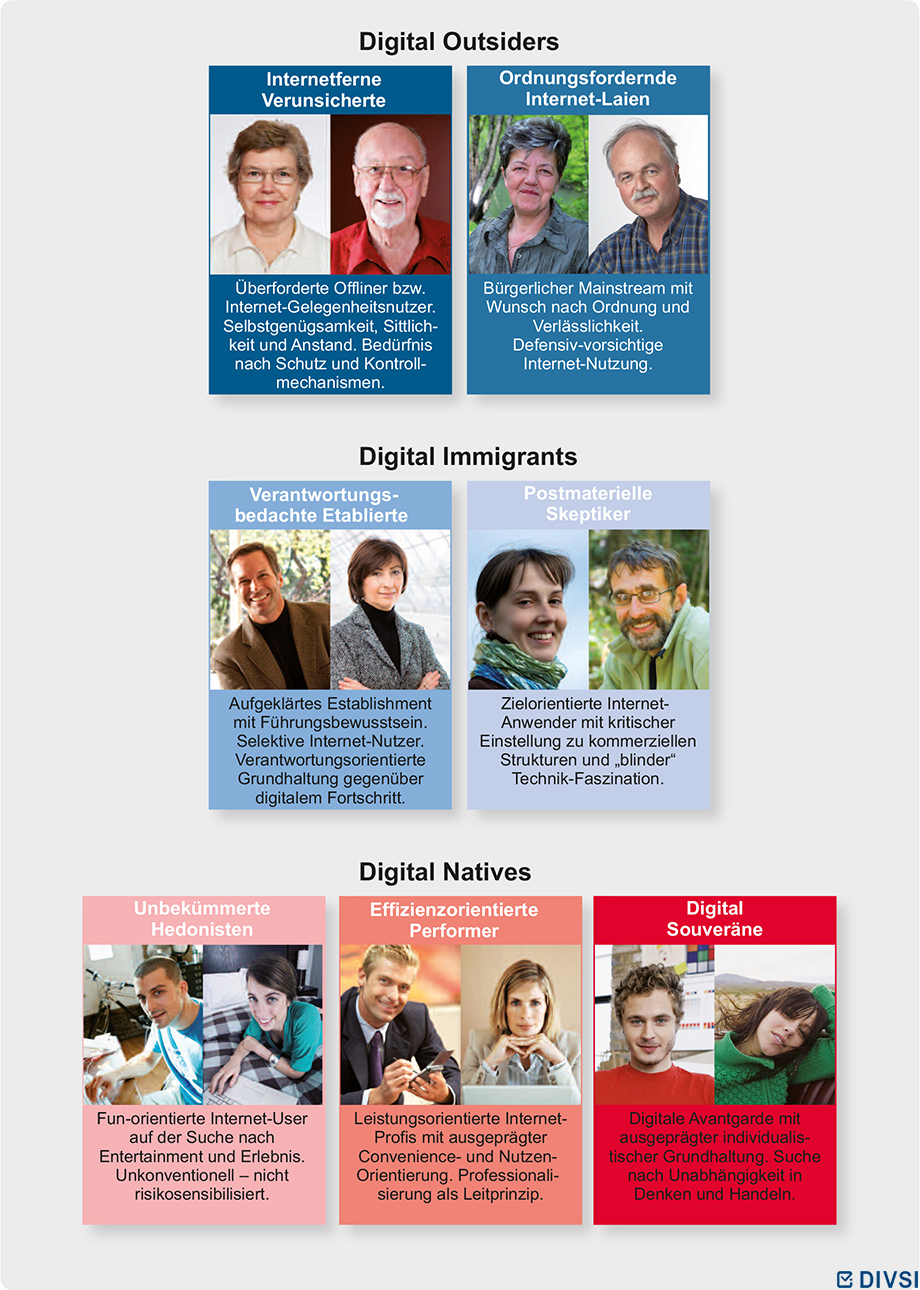
\includegraphics[width=0.9\textwidth]{DIVSI-Milieus.jpg}
\caption{Internet Milleus as defined by DIVSI \cite{divsi2012divsi}}
\label{fig:divsi_milieus}
\end{figure}

\begin{description}[leftmargin=0cm]
\item[Digital Souver\"{a}ne] This group moves naturally on the Internet and is therefore exposed to phishing. They also often use smartphones. We rule them out because they think that they already know the problems of the Internet and hence they would reject a training offer anyways. In fact, this group will likely never download the app.
\item[Effizienzorientierte Performer] This group matches our preconditions because they are using the Internet as well as smartphones. In contrast to the previous group, they are interested in learning something new and see their own learning as an investment in the future. To target this group we should show that you can learn something from this app.
\item[Unbek\"{u}mmerte Hedonisten] This group is also native in the digital worlds but in contrast to the before mentioned groups are not aware of the problems and frauds therein. When they are aware of the problems they seek to secure themselves with automated software instead of concerning themselves with it. Therefore, they are not motivated to use our app.
\item[Postmaterielle Skeptiker] This group is interested in the Internet and uses it frequently. On the other hand they are aware that there are problems and frauds. As they are interested in information on the Internet especially from official sources they might download our app. To target this group we should clearly state that this app is from an university.
\item[Verantwortungsbedachte Etablierte] This group is online regulary and also uses smartphones. They are especially interested in using protection software and actively search information on the Internet. The users of this group do not think that they could protect themselves from the dangers of the Internet and actively seek to change this. Therefore they most likely will appreciate the app. To target this group we should clearly state that this app helps the user to protect himself.
\item[Ordnungsfordernde Internet-Laien] These users are using the Internet rarely. Because of this they are particularly careful when using the Internet and normally do not enter personal data. Therefore, it is not likely that they will use the app. Besides, they usually do not have smartphones.
\item[Internetferne Verunsicherte] These users do not use the Internet. Therefore, they are not exposed to phishing threats.
\end{description}

\begin{figure}[hHtbp]
\centering
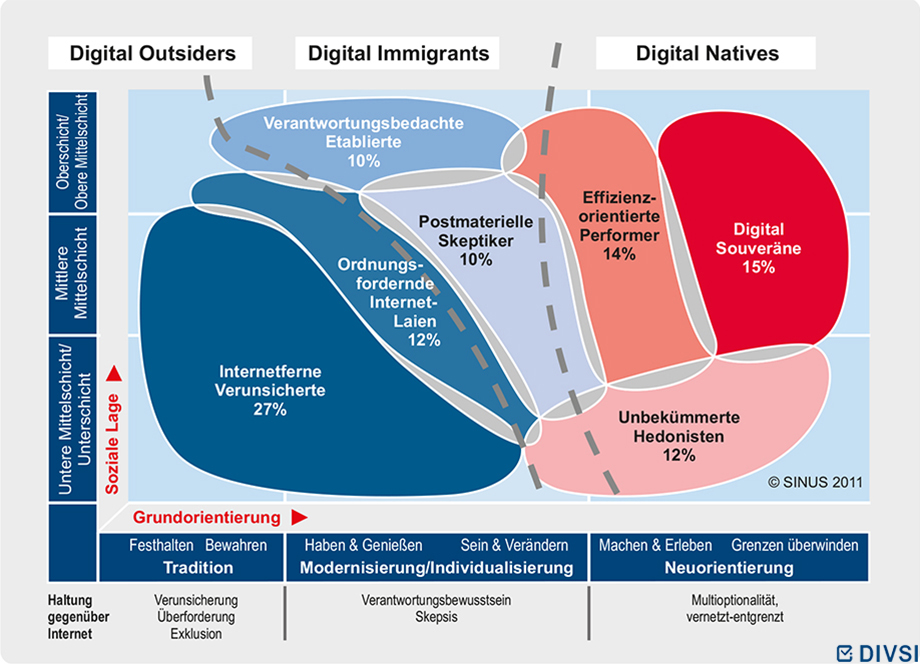
\includegraphics[width=0.56\textwidth]{DIVSI-Kartoffeln.jpg}
\caption{Internet Milleus as defined by DIVSI}
\label{fig:divsi_kartoffeln}
\end{figure}

In conclusion, we consider \textit{Verantwortungsbedachte Etablierte} (10\%),  \textit{Postmaterielle Skeptiker} (10\%),  \textit{Effizienzorientierte Performer} (14\%). In total these are 34\% of the german population.
	%*******************************************
\section{Phishing Survey}
%*******************************************
\label{s:prestudy}
Before elaborating on the concrete app design we ran a small phishing survey.
 To the best of our knowledge there do not exist other surveys which resemble ours and additionally were conducted in Germany.
 This chapter deals with the main objectives of the survey.
 Furthermore, it provides some details and finally presents the results and evaluates the questionnaire.


%============================================
\subsection{Main Objectives}
%============================================
Our main objectives of this survey were twofold:

\begin{enumerate}
	\item \textbf{Awareness and Knowledge} One goal of the survey was to comprehend what exactly Internet users understand under phishing.
 With a Likert scale we furthermore tried to figure out how they evaluate their on knowledge on the topic of Internet security.

	\item \textbf{Preferences of Users} Another purpose of the survey was to get an idea of the users' preferences with regard to an educational app.
 For example, they were asked whether they found a quiz based game appropriate for learning purposes.

\end{enumerate}
%============================================
\subsection{Survey Details}
%============================================
This section provides some details about our questionnaire, how we distributed it and how we filtered the surveys in order to consider our target group for the results and evaluation.

\textbf{SURVEY IN APPENDIX???}

\subsubsection{Questionnaire}
In the following we present the structure of our questionnaire and the function of each section.
 
\begin{enumerate}
	\item \textbf{General Information} In this section the participant is asked to provide information regarding his gender, age, his professional qualification as well as his field of study or work.
 The main purpose of this section is to exclude participants which do not fit into our target group.

	\item \textbf{Internet Usage} Here, the participant is asked how often he uses the Internet, whether he owns a smartphone and which applications he uses on his desktop computer and which ones he uses on his smartphone.
 This section is intended to give us an overview of the users' Internet usage and helps us to exclude participants who do not fit into our target group.

	\item \textbf{Self-Assessment} In this part of the survey, the participant has to indicate how much he agrees to the presented statements with the aid of a Likert scale.
 The statements mainly refer to their self-assessment regaring their knowledge about Internet security.
 For example, they have to assess, whether they think they have enough knowledge, to avoid the dangers of the Internet or whether they think it is easy for them to distinguish legitimate e-mails from fake ones.
 This section is partially based on Likert scale statements used by DIVSI \textbf{..ADD REF}
	\item \textbf{Phishing} Here, the participant gets concrete questions to the topic of phishing.
 In particular, he is asked which services and which user information are endangered by phishing attacks.
 This section purposes to find out what the participants know about and think of phishing.

	\item \textbf{Anti-Phishing App} This section asks the user for his preferences regarding an anti-phishing education app.
 With the aid of a Likert scale he is requested to assess, for example, whether the would like having a game with a fish, or whether he finds a text-based approach meaningful as well as whether he would have fun with a question-answer quiz game.

	\item \textbf{Further Survey Progress} In this part of the survey the user can provide us his e-mail address in case he wants to get information about the further progress of the survey or would like to test the app.

\end{enumerate}

\subsubsection{Distribution}
In total 251 persons participated in our survey.
 We set up an online survey as well as asked students to fill out our printed survey.
 In the following we briefly explain our distribution process.


\begin{description}
	\item[Printed Survey] To reach participants for our printed survey we contacted multiple professors and asked them whether we could have 10 minutes of their lecture time to have their students fill out our printed survey.
 Moreover, we asked our friends and parents whether they can ask their friends, colleague or customers to fill out the questionnaire.

	\item[Online Survey] The online survey was mainly distributed digitally.
 We contacted our friends and asked them to participate in the survey.
 We also demanded to forward the link to their friends so we could reach a wider range of people.

\end{description}

\subsubsection{Filtering for Evaluation}

The following Table~\ref{table:prestudy_filter} summarizes what kind of answers we used in order to exclude participants from the survey who do not fit into our target group.
\label{table:prestudy_filter}
\begin{center}
    \begin{tabular}{ | p{5cm} | p{10cm} |}
    \hline\textbf{Question} & \textbf{Filtering}  \\  \hline
		\hline\  Age & We consider all adults ranging from 18 - 65 years.
 \\
    \hline\  Gender & We do not exclude any gender.
 \\ 
    \hline\  Professional qualification & The participant does not have to exhibit a specific professional qualification to be considered for the results and evaluation.
 \\ 
		\hline\  Field of study/work & Students, employees or employers in the field of computer science or electrical engineering are filtered out as they do not belong to our target group.
 \\ 
	  \hline\ Frequency of Internet usage & Participants who have indicated ``rarely'' as the answer to this question do not belong to our target group and thus are filtered out.
 \\ 
	  \hline\ Used Internet applications  &  The listed applications include, for example, browser, e-mail, shopping as well as banking.
 Any service of the Internet is potentially endangered by phishing.
 For this reason we do not use this question to filter out participants.
\\ 
    \hline\ Owning a smartphone  & With the app we particularly target smartphoner owners.
 For this reason participants who do not own any kind of smartphone are filtered out.
 \\
		\hline\ Used smartphone applications in the Internet  & The listed applications include, for example, browser, e-mail, shopping as well as banking.
 Any service of the Internet, especially on a smartphone, is potentially endangered by phishing.
 For this reason we do not use this question to filter out participants.
 \\
    \hline\ Number of received commercial e-mails per week  & We do not filter out any participant with this question.
 \\
    \hline\ Number of received e-mails asking for personal data  & We do not filter out any participant with this question.
 \\
    \hline\ User reads up on topics related to dangers in the Internet  &  Participants who have chosen ``no'' as answer are filtered out.
 We specifically target users who are interested in getting safer in the Internet.
 As the participants who have indicated ``no'' do not seem to have any interest in doing so, they will most likely do not show interest in our app.
 For this reason we regard them as not belonging to our target group and exclude them from the analysis and evaluation.
\\
    \hline\  Section to self-assessment regaring their knowledge about Internet security &  We do not filter out any participant with these statements.
\\
		\hline\  Section to questions concretely related to phishing & We do not filter out any participant with these statements.
 \\
    \hline\  Section to preferences for an anti-phishing education app & We do not filter out any participant with these statements.
\\
    \hline
    \end{tabular}
		
\end{center}
%%%%%%%%%%%%%%%%%%%%%%%%%%%TO ADD: CAPTION AND LABEL (UND OBEN REFERENZIEREN)%%%%%%%%%%%%%%%%%%%%%%%

In the following section we present and evaluate the results of the study.
 With the filtering above we had 169 remaining participants who were considered for the evaluation.

%============================================
\subsection{Results and Evaluation}
%============================================
The studey yielded interesting results which should be considered when designing an anti-phishing education app, either for this work, or if not possible due to time constraints in future work.
 This section outlines the results of the study.


\begin{description}[leftmargin=0cm]
	\item[General Information] The ratio of our male and female survey participants was more or less balanced.
 40.83\% of the users were female and 56.80\% of them were male.
 The remaining 2.37\% did not indicate any gender.
 The average age of our participants is 27.59, the youngest participants are 19 years old, the oldest are 63 years old.
 Most of the survey participators, 48.52\%, obtained a university degree.
 24.85\% of them do not have any professional qualification (yet). 17.75\% did an apprenticeship and the remaining participants had a master craftsman certificate or did not indicate any professional qualification in the survey.
	
	\item[High Rate of Android Users] The majority of the participants were Android users.
 In total about 60\% of the study participants use an Android smartphone.
 The remaining 40\% are iOS users.
 This result additionally supports our decision for the implementation of an Android application.

	\item[High Internet Usage Frequency] 51.48\% of the users are online several times a day.
 Another 30.18\% indicated that they are online even constantly.
 As a consequence, over 80\% of the survey participants are frequently online.
 This is depicted in Figure~\ref{fig:internet_usage} Being online is always connected with being attackable and vulnerable to dangers of the Internet, such as phishing attacks, while the extent of the vulnerability of course depends on the expertise of the person being online.
 However, the more often a user is in the Internet, the more likely it is that he will experience a phishing attempt.

	
	\item[Usage Distribution of Internet Applications] Figures~\ref{fig:desktop_apps}~and~\ref{fig:smartphone_apps} summarize the usage distribution of Internert applications on a desktop computer and on smartphones.
 Almost all participants, 99.41\%, make use of e-mails on their desktop computer.
 88.76\% of the smartphone owners use their e-mail application on the smartphone, which is still a high percentage.
 As we have previously mentioned, cf.
~Section~\ref{s:attack_channels}, e-mail is a common attack channel for phishing attempts.
 Consequently, all users of e-mail applications as well as users of webmail on mobile phones are potentially endangered by phishing attacks.
 The same applies to participants using browsers.
 A common way to trick users to disclose their confidential information is the use of fake websites.
 These websites can be reached by clicking on a link in an e-mail, SMS or in online social networks or instant messaging systems as well as by simply surfing in the Internet.
 About 80\% of all considered participants make use of desktop or smartphone browsers.
 Furthermore, it is conspicuous that banking is far less used on the smartphones compared to desktop computers.
 While about 74.56\% of the participants make use of online banking on the desktop computer, only 26.63\% make use of it on their smartphones, which is however still a quarter of the participants.
	The question to ask here is if these users use the browser for the online banking or if they use apps provided by their bank.
 Regardless of the answer to this question, these users might be more likely to react to phishing e-mails, claiming to come from their bank, on their smartphone compared to other users who manage their financial arrangements on a desktop computer and thus are less likely to access a phishing website, cf.
~Section~\ref{s:antiphishing_on_smartphone}. To sum it up, all the categories of applications are used by the participants, on their smartphones as well as on their desktop computers.
 For this reason, all of these application categories should be reflected in the choice of the example URLs for the final app.
 For future work, one could argue to put the focus on URLs from specific categories (also those which were not considered for the study), depending on the usage distribution.


	\item[Self-Assessment - Knowledge to avoid dangers of Internet] With a Likert scale the participants had to indicate how much they agreed with the following statement: ``I have enough knowledge to avoid the dangers of the Internet''. 18.34\% of the participants strongly agree with this self-assessing statement.
 Further 45.56\% agree with the statement and only about 13\% disagree or strongly disagree with this statement.
 As a consequence the majority of the participants were quite confident that they could avoid the security-related risks raised by the Internet.
 
	
	\item[Self-Assessment - Distinguish legitimate from illegitimate e-mails] With a Likert scale the participants had to indicate how much they agreed with the following statement: ``I find it easy to distinguish legitimate e-mails from fake ones''. Here, 37.23\% of the participators strongly agreed with the statement and even 50\% of them agreed with it.
 Only about 8\% of the participant did not agree or strongly disagreed with this statement.
 This arouses the suspicion that the users are not aware of how easy it is to spoof the ``from'' field of an e-mail or to create credible message contents which in fact may persuade the receiver to be trustful.

	
	\item[Self-Assessment - Trust to e-mails from known parties]  With a Likert scale the participants had to indicate how much they agreed with the following statement: ``I trust e-mails which come from persons I know''. The majority of the participants trust e-mails which come from persons they know.
 Approximately 20\% strongly agreed and approximately 57\% agreed with this statement.
 Only about 2\% strongly disagreed and approximately 5\% of the participants disagreed with this statement.
 This agains shows, that most of the participants are not aware that spoofing the ``from field'' of an e-mail is very easy.
 These users are likely to react to e-mails which claim to be, for example, from friends.
 Such e-mails may contain links to the download of malware or malicious websites.


	\item[Self-Assessment - Internet security is only related to financial applications] With a Likert scale the participants had to indicate how much they agreed with the following statement: ``Internet security is only related to financial applications''. The answers to this statement showed that the majority of the participants are aware that security related issues in the Internet do not solely concern financial applications.
 49.7\% of the users strongly disagreed with this statement and another 24.26\% disagreed.
 Only about 10\% of the participators agreed or strongly agreed with this statement and about 14\% indicated ``neither nor'' as an answer.
 Even though most users seem to be aware that Internet risks do not only concern financial applications, the ones who are not aware that, phishing for example, can also occur in online social networks, should be enlightened about this.
 To do this, originally, our plan was to display the consequences of falling for a certain phishing website (phishing URL). In this way, the user could have learnt what his loss could have been, if he had fallen for such an attack in reality.
 This would have contributed to his awareness that security issues in the Internet, in this particular case phishing, are not necessarily related to financial loss only.
 Due to lack of time we could not realize this approach, so it is something which should be considered in future work.


	\item[Services endangered by phishing] Figure~\ref{fig:endangered_services} summarizes the results for this question.
 All in all, we can observe that the participants agree that phishing can actually occur related to any service.
 The users agree (97.04\%) that especially the e-mail service is endangered by phishing.
 Also they see the browser with fake websites (70.41\%), online banking (83.43\%) as well as social networks (74.56\%) as endangered.
 Still about 40\% consider various media (audio and video) services as well as online games as endangered.
 These services are in fact not targeted as often as other services in the Internet, however they are potential targets and should be communicated to the user, for example, with the aid of the choice of the URLs to decide on.

	\item[Data endangered by phishing] Figure~\ref{fig:endangered_data} outlines the results of this question and illustrates that the participants agree that every kind of data is endangered by phishing attacks.
 90.53\% of the participants are of the opinion that login data is endangered by phishing.
 About 89\% agree that credit card information as well as personal data is endangered, too.
 Finally, 76.33\% of the participants consider PINs and TANs endangered.
 Consequently, there does not seem to be a major necessity in enlightening users in this area.

	\item[Preferences for an education app] todo.
 evtl nochmal aufteilen
	%\item[VERGLEICHE?]
\end{description}


\begin{figure}[hHtbp]
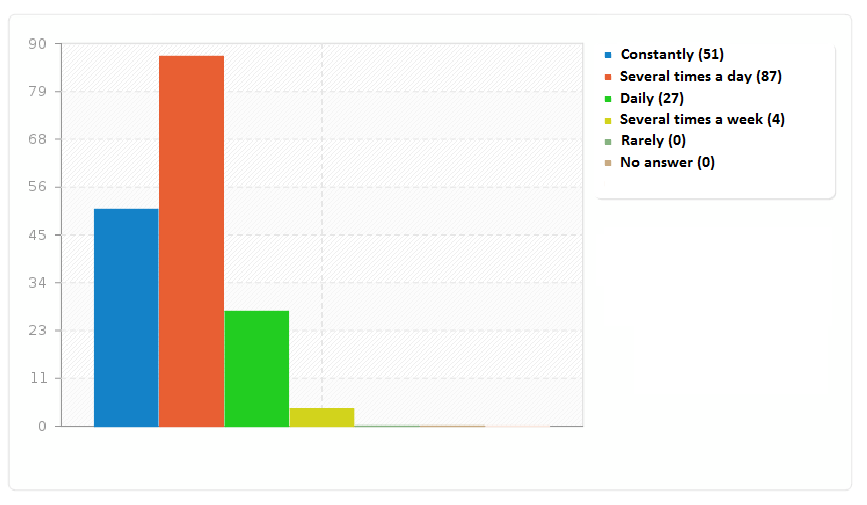
\includegraphics[width=1.0\textwidth]{graphix/internet_usage.png}%
\caption{Frequency of Internet Usage}%
\label{fig:internet_usage}%
\end{figure}


\begin{figure}[hHtbp]
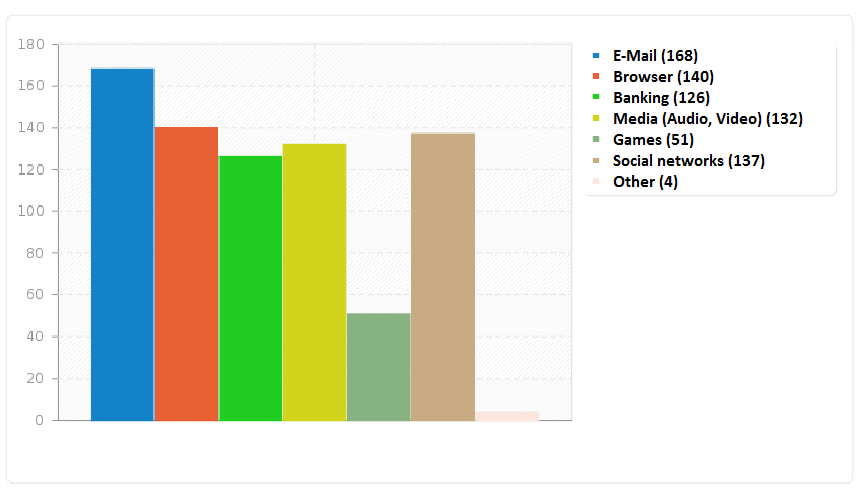
\includegraphics[width=1.0\textwidth]{graphix/desktop_applications.png}%
\caption{Usage of Internet Applications on Desktop Computers}%
\label{fig:desktop_apps}%
\end{figure}

\begin{figure}[hHtbp]
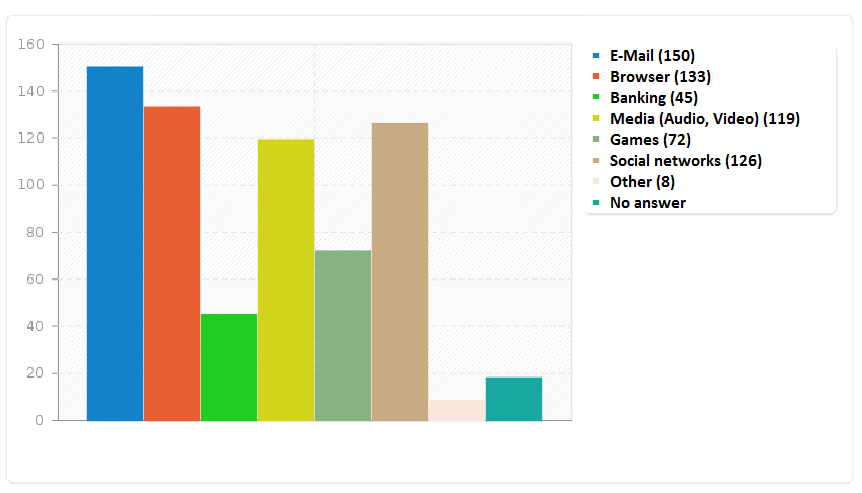
\includegraphics[width=1.0\textwidth]{graphix/smartphone_applications.png}%
\caption{Usage of Internet Applications on Smartphones}%
\label{fig:smartphone_apps}%
\end{figure}

\begin{figure}[hHtbp]
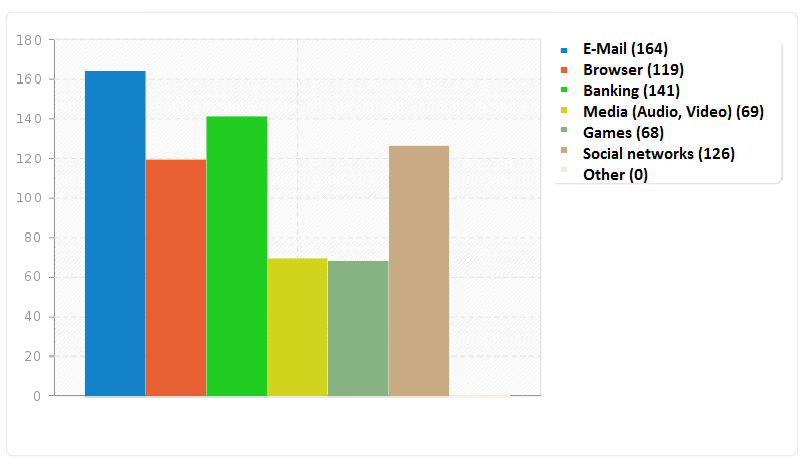
\includegraphics[width=1.0\textwidth]{graphix/endangered_services.png}%
\caption{Services Endangered By Phishing}%
\label{fig:endangered_services}%
\end{figure}

\begin{figure}[hHtbp]
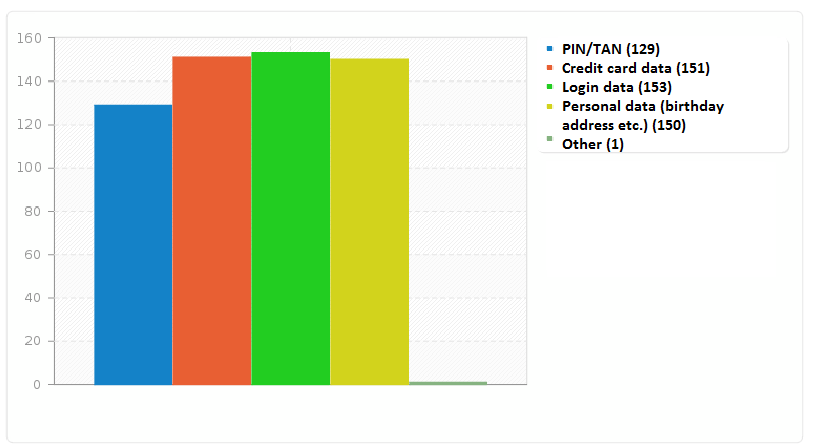
\includegraphics[width=1.0\textwidth]{graphix/endangered_data.png}%
\caption{Data Endangered By Phishing}%
\label{fig:endangered_data}%
\end{figure}

	%*******************************************
\section{Teaching and Learning Content}
%*******************************************

\textbf{TEILE VON DIESEM KAPITEL SCHEINEN NACH MELANIE EHER BACKGROUND ZU SEIN: SCHAUEN}
In this section we will describe and elaborate on different teaching and learning contents which can potentially be communicated to the user.
 At the same time we will reason our decision whether to communicate the specific content or not.

%Documents master_thesis/notes/android_browser bla -> BEGRÜNDUNG WARUM manches nicht sinnvoll ist (diese Sachen vielleicht eher in Appendix vor allem versionsunterschiede)
%Documents master_thesis/konzepte/android browser elemente UND browser comparison
%CHECK IF I FORGOT SOMETHING!!!!
%===========================================
\subsection{Phishing URLs}
%===========================================
As aforementioned, we focus on teaching the user how to analyze a given URL and to decide on it whether it belongs to a legitimate or illegitimate website.
 In order to distinguish legitimate URLs from phishing URLs it is necessary to analyze existent phishing URLs regarding how the URLs are spoofed in order to deceive the users.
 For the analysis of phishing URLs we chose the database of PhishTank.

PhishTank is a free community site where people can submit, verify and view phishing data.
 It provides an API which makes all PhishTank data accessible.
 Renowned organizations such as Yahoo, Kaspersky Lab and Mcafee use the data submitted by PhishTank~\cite{phishtank}. A further deciding reason to choose PhishTank as our phishing URL database was that Kaspersky Lab itself recommended us to make use of it for our URL analysis.
 For the phishing URL analysis we made use of the URL categories which had been identified by the authors of Anti-Phishing Phil~\cite{sheng2007antiphishingphil} as a starting point.
 To these belong IP address URLs, subdomain URLs as well as similar and deceptive domain URLs.
 With these given categories we tried to assign the PhishTank URLs to the available categories.
 When no category suited the URL to be assigned, we generated a new category, to which the URL could then be assigned to.
 In addition we found various categories mentioned in literature, which we also included to our categories, even if we could not find any explicit example URL in the PhishTank database.
 In the following the identified URL categories are explained.


%...........................................
\subsubsection{Phishing URL Categorization}
%...........................................
\label{s:url_categories}
URLs are complex and many users do not know how exactly they have to be interpreted.
 For example, users can be convinced about the authenticity of an URL when it contains the brand name anywhere.
 Phishers exploit this lack of knowledge in different way.
 In the following we present the identified spoofing attacks on URLs and state whether they are covered by the app.

\begin{description}[leftmargin=0cm]
	\item[Subdomain] Phishers make use of subdomains which are very similar or even identical to the domains of the spoofed target institutions.
 This makes the users believe that they are on a legitimate website.
 This form of URL spoofing is covered by our education app.

	\item[IP Address] Sometimes phishers do not even bother registering any domain at all.
 In this case, the URL to the phisher's fake website contains an IP address.
 This form of URL spoofing is covered by our education app.

	\item[Nonsense Domain] We frequently encountered URLs which had registered quite nonsense as their domain.
 The domain names ranged from random letters to domain names like ``marketstreetchippy.
com''. Sometimes other parts of the URL contained the brand name, but sometimes there was no clue in the URL about to where it is actually leading.
 This form of URL spoofing is covered by our education app.

	\item[Trustworthy, But Unrelated Domain] Some URLs are very well-crafted.
 When reading them they appear meaningful and trustworthy.
 This is particularly accomplished by making use of domain names which sound very trustworthy, for example, ``account-information.
com'', ``secure-login.
de'' or ``security-update.
com''. If the URL additionally contains the brand name of the target institution somewhere in the URL the user can be perfectly deceived.
 This form of URL spoofing is covered by our education app.

	\item[Similar and Deceptive Domains] Another possibility to fool users with a spoofed URL is to use URLs which look like the original ones, but have a slight difference.
 For example, phishers register domains which resemble the targeted domain, but has a typo.
 To spoof ``paypal.
com'', for instance, the attacker might register ``paypel.
com''. Another approach is to use a modification of the original domain.
 The modified domain contains the brand name in some form.
 For example, ``facebook-login.
com'' can be registered in order to fake ``facebook.
com''. Finally, the attacker can scramble letters of the original domain, which can be very hard to detect at first sight.
 This form of URL spoofing is covered by our education app.

	\item[Homograph Attack] The homograph attack exploits character resemblance.
 Here characters are replaced by other characters which look very similar to the replaced one.
 For example, an attacker might replace a ``w'' within a genuine domain with ``vv'' and register it.
 An even more advanced way is to replace characters of the genuine domain with characters from other langauge sets, such as Cryllic languages, where the characters will look almost identical~\cite{gabrilovich2002homograph}. The letter case is indistinguishable for the human eye in many cases.
 For this reason only cases that are distinguishable by the human eye are covered by the educational app.

% DAS WAS DER USER NICHT SEHEN KANN WIRD NATÜRLICH AUCH NICHT GECOVERED WERDEN KÖNNEN
	\item[Tiny URLs] A tiny URL service is used to convert a long URL into a short one.
 Due to their shortness tiny URL are very comfortable to use and easy-to-type.
 There seemed to be a trend of using tiny URLs for phishing in 2009, in particular in instant messaging services.
 Tiny URLs usually do not give a hint about the target website and users do not tend to be suspicious about receiving such links from a ``friend'' what made the use of it quite popular~\cite{tinyurlpcworld}. Tiny URLs redirect the tiny URL to the actual long URL.
 As we consider the ``analyze URL after-click'' scenario for the user education, there is no need of the tiny URL to be covered by the app.

		\item[Cloaked URLs] Other phishers integrate an ``@'' into the URL so that domain names become difficult to understand and the actual destination of a link becomes ``cloaked''\cite{alnajim2009fighting}. For example, the URL http://paypal.
com@google.
com/ is redirected to http://google.
com.
 As we consider the ``analyze URL after-click'' scenario for the user education, there is no need of the tiny URL to be covered by the app.

\end{description}

%...........................................
\subsubsection{Problems and Challenges With The Categorization}
%...........................................

%...........................................
\subsection{Smartphone limitation}
%...........................................
As already discussed in Section~\ref{s:antiphishing_on_smartphone} smartphones have several limitations, such as the small screen size. 
This section deals with the detection of phishing on the smartphone and the related limitations.
More particularly, we will briefly explain in which ways URLs can be checked with the smartphone and what kind of problems these operations raise.
Based on this we decided whether to communicate this kind of URL checking to the user or not.

\begin{description}[leftmargin=0cm]
	\item[Invisible Address Bar] Due to lack of space most of the smartphone browsers hide the address bar~\cite{amrutkar2012measuring} and use this won space for the web content. 
By doing this, not only potential security indicators are made invisible, but also the URL that indicates with which website the user is actually interacting.
In order to make the address bar re-appear the user generally has to scroll to the top of the whole website.
The fact that the address bar containing the important information of the URL is generally hidden must be communicated to the user.
Most of the users will probably know that they can access the address bar by scrolling to the top of the website.
However, for those who might not know how to deal with that an introduction is inevitable.

	\item[Analyze Complete URL Via Address Bar] Finding the address bar will not suffice for a reasonable URL analysis. 
Here again, the small screen size makes it is impossible to view the complete URL without any further action.
Specifically, it is necessary to first tap the URL address text and then scroll the pointer to the left and right for the URL analysis.
Without learning these steps a reliable URL checking is not possible. 
Therefore, these operations steps have to be communicated to the user.

	\item[Show URL Before Click] Many mobile e-mail clients provide the functionality of showing the URL a link leads to when touching and holding the link.
However, the Android stock e-mail app, for example, does not provide this functionality.
This operation is generally available in smartphone browsers for links on websites while surfing.
Yet, one should keep in mind that it might happen that the complete URL cannot be displayed on this preview in case it is too long. 
Consequently, as discussed in Section~\cite{s:coverage}, deceiving the user with well-crafted, illegitimate URLs becomes possible. 
In that section we have already extensively discussed the benefits and drawbacks of teaching the user how to preview the destination URL and have decided against it.

	\item[Copy and Paste URL] Previewing the destination URL raises flaws, such as there is no guarantee that every mobile e-mail client provides this functionality and deception remains possible. 
An alternative to the preview functionality is the copy and paste functionality.
When touching and holding a link, additional to the URL preview, the option "copy URL" is available.
Upon selecting this option the destination URL is copied to the clipboard.
Now the user may paste the destination URL to any editor or even the address bar itself in order to analyze the it \textit{before} submitting.
In case the URL was pasted directly into the address bar, left and right scrolling must further be applied for the analysis. 
Also, the user must be careful not to submit the URL before checking it, otherwise he also just could have clicked on the link and checked the URL afterwards.
Analyzing the URL in a separate editor would mean to re-paste the URL into the address bar afterwards and then submit it.
We believe that either of these steps are of too high effort and thus would not be followed by the users.
Also, the user would not be able to see the "real" target in case there is a redirect included. 
Hence, this kind of possible operation will not be communicated to the user.
\end{description}

%...........................................
\subsection{Browser Security Indicators}
%...........................................
As a matter for fact, there is a major lack of mobile browser security indicators~\cite{amrutkar2012measuring,trusteer2011}. 
Besides the lack of such indicators there is also the problem of inconsistencies among the mobile as well as desktop browsers.
This section deals with the security indicators of the Android standard browser which the user might potentially be told about.
Ultimately, our decision was not to tell anything about these security indicators, since they are too inconsistent even among the standard browser, depending on the device and Android version it is installed on.
\begin{description}
		\item[Https Padlock] The padlock in the browser chrome is a security indicator for the usage of https.
All Android standard browsers on various devices we have examined have a padlock on SSL secured pages.
Also, one should consider that there are illegitimate as well as legitimate websites where a padlock is part of the web content. 
Therefore, it is important to teach the users to look for the padlock in the browser chrome to verify that the site they visit is SSL secured, when they enter confidential data.
However, some browsers additionally make use of so called favicons, small website icons.
The danger of using such a favicon is that a phisher could use the image of a padlock~\cite{trusteer2011} in order to deceive the user.
Moreover, the padlock with/without favicon combinations appear in different ways. 
While a part of the standard browsers installed on various devices and Android versions we have examined only feature a padlock in case of https websites and no favicon at all, others make always use of favicons. 
In the latter case, if https is used the padlock is either displayed right next to the favicon or overlaps it .
Due to the variety of possible combinations as well as the deception potential in combination with favicons we decided not to tell the user about the padlock.
		\item[Touch Padlock] to see whole URL.
		\item[Certificate Verification]Tapping on the padlock icon results in an alert dialog where the user can select to view the certificate details ("show certificate").
Upon selecting this option details about the certificate will be displayed.
On the hand, while examining Android's standard browser on various devices and versions we have encountered that clicking on the padlock is not always possible. 
Hence, in these cases a validation of the certificate is not possible as well.
On the other hand, we consider the validation of certificates as out of scope for this work.
Therefore, this is an aspect which is not covered by our app.

\end{description}

%...........................................
\subsection{E-Mail Spoofing}
%...........................................

\begin{description}
	\item{From Field} not trustworthy
	\item{E-Mail Content} in hand of attacker
	\item{Links in E-Mails} do not necessarily go where it claims to go (not only in e-mail links).
\end{description}

\subsection{General Recommended Behavior}
\begin{description}
	\item[Do Not Click]
	\item[Do Not Download Attachment]
	\item[Look at URL]
	\item[Data Economy]
	\item[Date Entry Via Https]
	\item[Use of Https Within Websites] Browser
\end{description}

%...........................................
\subsection{Conclusion / Summary}
%...........................................

Summarize what to communicate to user here.
..


	
%*******************************************
\section{App Structure and Design}
%*******************************************
\label{s:approach}
This chapter presents our final approach for the app.
 In the following sections we elaborate on the app design.
In detail, we describe how we aspired to achieve our primary goals of increasing the security awareness and providing a service to educate the user on the topic of phishing with the aid of an app.
Afterwards, we describe what kind of common gaming elements are included in our app and give a rough overview to the course of the game.
Subsequently, we explain the specific teaching goals per level and how we decided to set the thresholds for unlocking the next level.
Finally, we provide a summary of basic learning principles and game techniques and to what extent these are reflected in our app.
%===========================================
\subsection{App Design}
%===========================================
\label{s:app_design}
We decided to divide our education app into two main parts.
 The first part is supposed to increase the security awareness of the users.
We also refer to it as ``awareness part''.
 The second part of the app then covers the actual educational blocks, also referred to as ``educational part''.
 The following listing summarizes the functions of our twofold app structure.

\begin{enumerate}
	\item \textit{Awareness Part:} The first part of the education app is intended to increase the user awareness regarding how easy it is to spoof e-mails and mislead users with such fake messages.
 This part is supposed to motivate the user to do something to counter the danger of the Internet and phishing, in particular.
It is covered directly after starting the app for the first time.
\begin{enumerate}
		\item \textit{Receive Fake E-Mail:} We want to illustrate to the user how easy it is to spoof the ``from field'' as well as the content of an e-mail.
 For this purpose, the user is displayed a form that allows him to enter a sender (an arbitrary e-mail address), a target e-mail address (user's e-mail address) as well as a text of his choice.
 Upon submitting the form the user will receive an e-mail from the e-mail address he had indicated as sender.
The body of the e-mail contains a common introduction and the user's text of choice.
 We believe that the user will be surprised about how easy even he himself could send a fake e-mail.
Hence, the user learns that he cannot fully trust the ``from field'' and the content of the e-mails he is receiving.
The template for this e-mail can be found in \autoref{a:mail}.
		\item \textit{Link Text Unequal Target URL:} The awareness part of the app is also supposed to show the user that he cannot trust the texts of a link he is clicking on.
 To illustrate this, the user is asked to click on a link with the text ``https://www.google.de/''. Clicking on this link, the user will expect to land on the Google website, what will not happen.
 In fact, the user is linked back to our app, where he is told that link texts are not trustful as well.
 
	\item \textit{Fake Website:} Finally, the user is told that creating a copy of a website is also very easy.
 He is told that a reliable way to decide whether a website is a fake or not is to analyze the URL of the website he is visiting.
Ultimately, he is told that this will be the focus of the following exercises.

\end{enumerate}
	\item \textit{Educational Part:} The second part of the app covers the actual educational part.
 Here, the user is learning about various spoofing techniques of the attacker. The second part of the app is divided into levels of increasing difficulty.

\begin{enumerate}
	\item \textit{Learning Part:} 
The users are first introduced to the lessons to be learned for the current level.
These lessons are generally delivered with simple text.
Sometimes screenshots or graphics are included.
 The learning contents of each level are described in \autoref{s:knowledgetransferperlevel}.
		\item \textit{Exercise} After every introductory block on each level, a corresponding exercise section follows (cf. \autoref{s:knowledgetransferperlevel}).
		\item \textit{Increasing Difficulty:} There is an increase of difficulty for each succeeding level.
 That is to say, in each level the tasks become more difficult to accomplish (cf. \autoref{s:knowledgetransferperlevel}).
\end{enumerate}
\end{enumerate}


%===========================================
\subsection{Gamification}
%===========================================
There exist several game elements which are widely used in most modern games.
These game elements are reflected in our app as follows:

\begin{description}[leftmargin=0cm]
\item[Lives:] An inherent property of a game is the possibility of losing it.
If a player is not able to lose a game he will get no positive feedback on having won it.
At the same time, one does not want the player to lose the game directly as the result of one minor mistake.
Therefore, most games have some kind of ``you have N tries''-element, which is commonly referred to as ``lives''.
We included such a mechanism in our app.
The details are layed out in \autoref{s:game_rules}.
\item[Levels:] Most games have some kind of level system.
This serves multiple purposes.
First, it is important for the player to get a feeling for the progress he makes.
Second, it provides fixed points in the game from where he can restart or pause and continue later on.
The details of the leveling strategy can be found in \autoref{s:leveling}

\item[Achievements:] There exists a type of player who is willing to invest a lot of time in a specific level in order to finish it perfectly or to find every hidden secret in it.
To address this type of player modern games offer so called ``achievements''.
Achievements are special elements of a game that a player can unlock if he, for example, finds a special object or if he plays a given level exceptionally well. 
We implemented achievements for logging in with google+, completing each introductory level and finding 5, 10, 25, 50, 100 and 500 phishing URLs. 

\item[Leaderboards:] Finally, games often have a leaderboard.
A leaderboard is an area where a player can compare his progress in the game with the one of other players.
For many people such a leaderboard have a significant impact on their motivation and engagement resulting in striving for a better performance.
We introduced two leaderboards:
\begin{enumerate}
\item \textit{Total Points:} We have a leaderboard that shows how many points the player gained while playing a level. The details of how the points are calculated are described in \autoref{s:leveling}.
\item \textit{Detected Phishing URLs:} We also introduced a leaderboard which displays the user who has detected the most phishing URLs in the app. 
\end{enumerate}

\end{description}

%===========================================
\subsection{Course of the Game}
\label{s:game_rules}
%===========================================
The educational part, which follows the awareness part, is divided into several levels.
This section discusses the course of the game in the educational part.
 In each level the user is provided with a specific introductory block.
 After this lecture part is consulted by the user, he has to finish the corresponding exercise.

The first and second information blocks (introduction part 2 and level 1) as well as their corresponding exercises differ from the ones of the other levels. Here, the users obtain basic knowledge in order to balance out inequalities concerning the varying previous knowledge of the players, before the actual game begins.

\begin{description}[leftmargin=0cm]
	\item[Obtaining Basic Knowledge:]  
The first information block and task of the user (introduction part 2) deals with accessing the address bar of a webbrowser and viewing its URL completely (cf. \autoref{s:knowledgetransferperlevel}).
 After successful completion the user is linked back to the app and level 1 begins.
 From this level on, the user has three lives upon the start of each level (cf. \autoref{fig:Screenshot_urltask}).
 In level 1 he has to identify the domain of valid URLs (cf. \autoref{s:knowledgetransferperlevel}).
 In this level wrong answers result in both, losing points and losing a life.
 Generally, the user can never get less than 0 points in order to keep him motivated.
 When the user has no more lives left he has to restart the current level.
 With every correct answer the user gains points.
	\item[The Actual Game:]  In level 2 we start introducing URL spoofing techniques. 
All exercises which are followed by the introductory blocks are structured as follows from this point: the user is presented a URL.
The user has to scroll the URL to the very left in order to analyze it completely.
The scrolling is supposed to simulate the behavior of a browser.
The user has to decide whether the presented URL is a phish or a valid URL, by either clicking on the cross or the check mark respectively.
The user interface of this challenge part is depicted in \autoref{fig:Screenshot_urltask}.
 Similar to level 1, the user can lose and win points, lose lives and might have to restart a level.
\autoref{fig:lose_points_life} illustrates the game flow and consequences of wrong and correct answers from level 2-8.
 If the user has correctly identified a phishing URL, he has to mark the domain to prove that he has understood the concept.
An example view of this proof part is depicted in \autoref{fig:Screenshot_proof}.
 In all other cases the user is directly shown the result of his answer.
 We decided that rejecting valid URLs is not as severe as accepting phishing URLs.
 For this reason the penalty for accepting a phishing URL is stricter (loss of points and a life) than the one for rejecting a valid URL (loss of points).
 In summary, the user generally loses points for wrong answers, but he does not lose a life for every wrong answer.
 All in all, the user loses points and a life in the following cases: the user has falsely accepted a phishing URL or the user has correctly rejected a phishing URL, but could not mark the domain correctly. In all other cases of wrong answers the user cannot lose lives, but only points.
For correct answers the user is rewarded with earning points and eventually finishing the current level.
\end{description}


\begin{figure}[hHtbp]
\centering
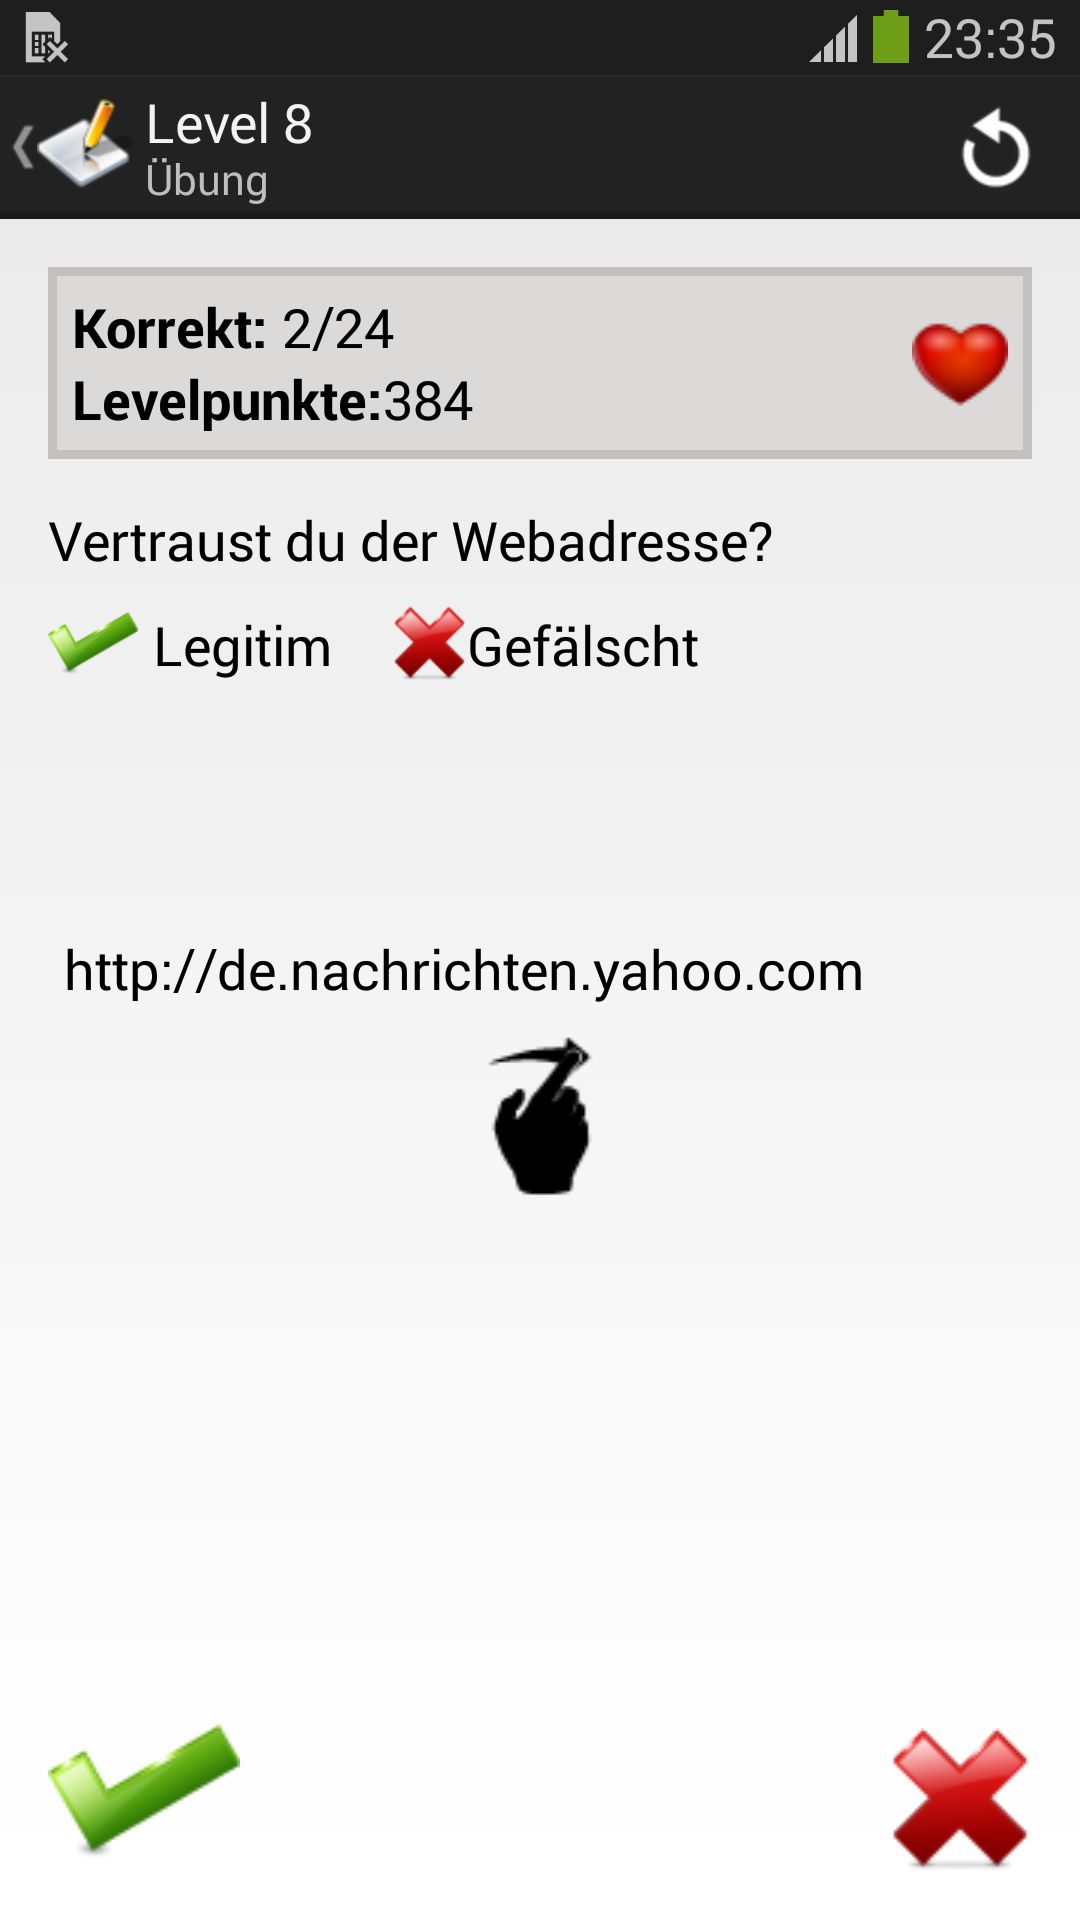
\includegraphics[width=0.4\textwidth]{Screenshot_urltask.png}
\caption{Example challenge view where the user has to decide whether the URL is a phish or not by clicking on the cross or check mark respectively. The user has 3 lives and has to scroll the URL in order to analyze it.}
\label{fig:Screenshot_urltask}
\end{figure}


\begin{figure}[hHtbp]
\centering
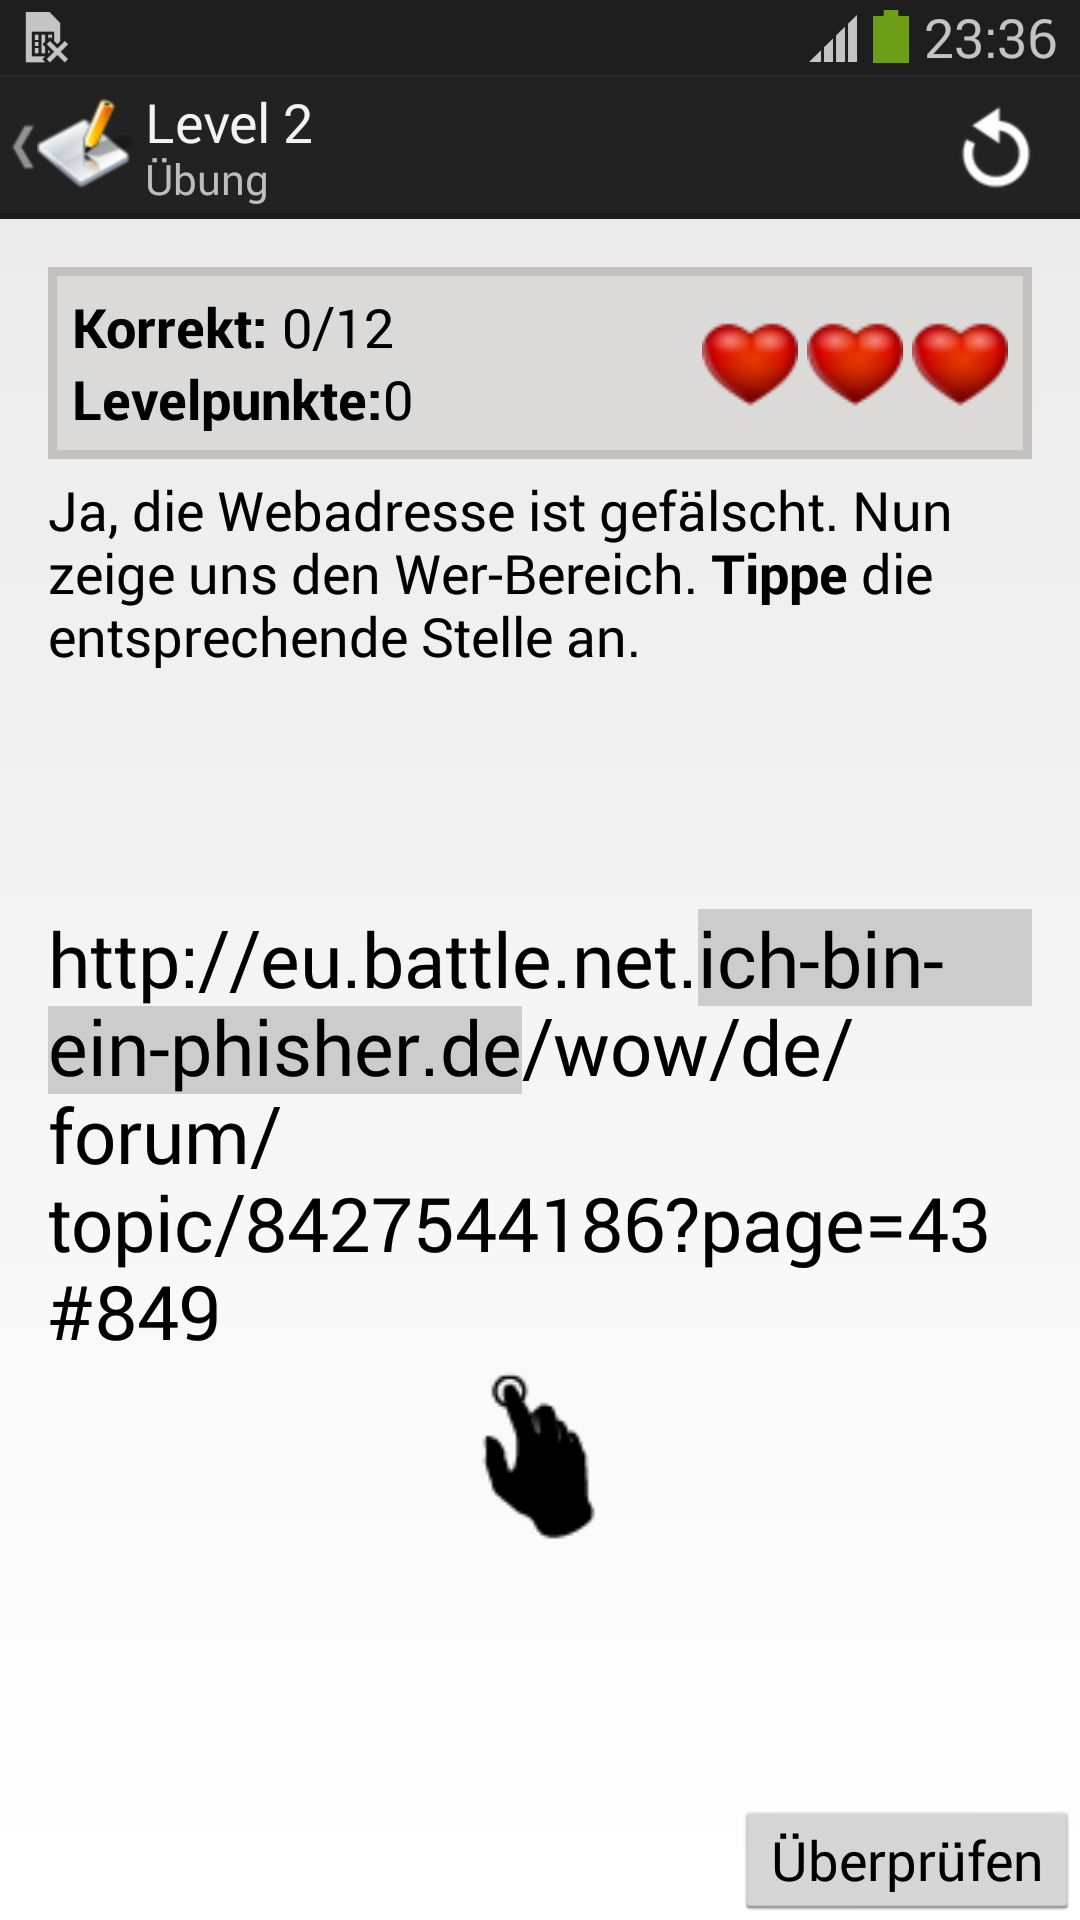
\includegraphics[width=0.4\textwidth]{Screenshot_proof.png}
\caption{Example view where the user has to mark the domain after correctly identifying a phishing URL}
\label{fig:Screenshot_proof}
\end{figure}

\begin{figure}[hHtbp]
\centering
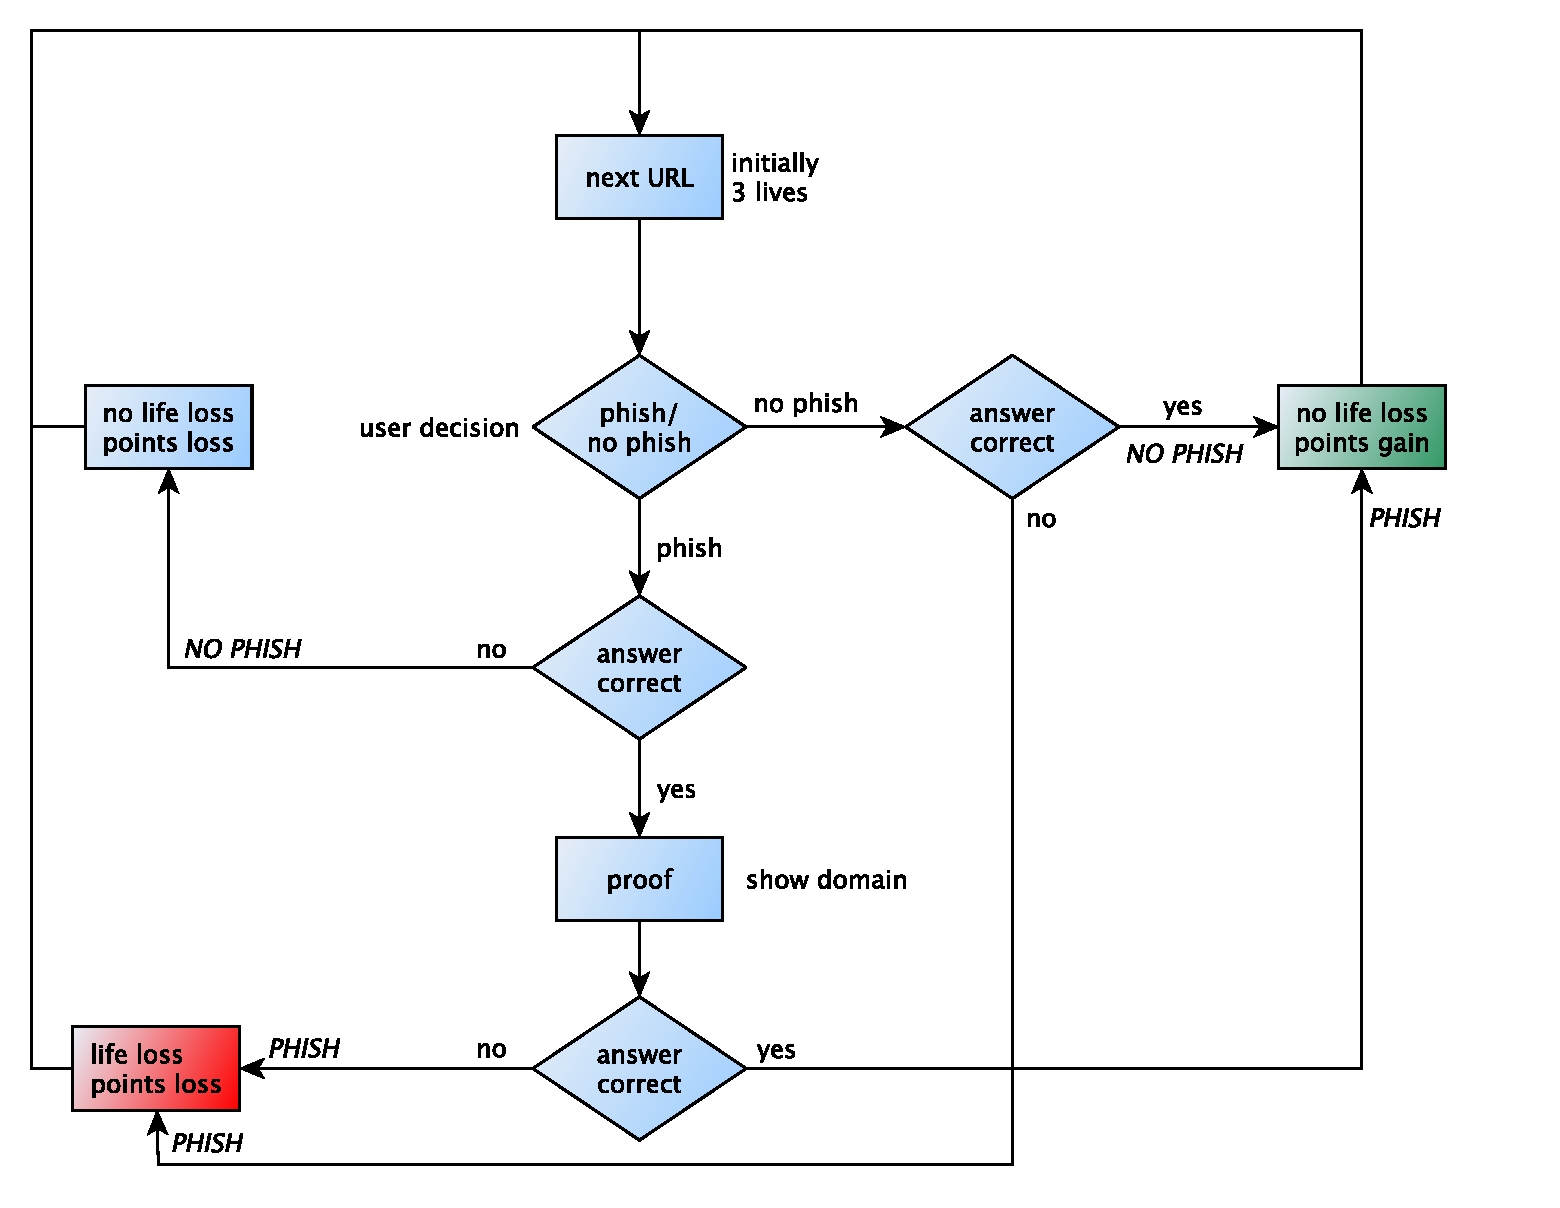
\includegraphics[width=1.0\textwidth]{lose_win_points.pdf}
\caption{Losing points and lives in the game (levels 2-8). PHISH/NO PHISH refers to whether the displayed URL is a phish or not. In case the terms are not capitalized, i.e. phish/no phish, they refer to the user's decision.}
\label{fig:lose_points_life}
\end{figure}

%===========================================
\subsection{Teaching Goals per Level}
%===========================================
\label{s:knowledgetransferperlevel}
This section summarizes the learning objectives of each level.
 Note that we generally do not use technical terms like URL, domain, subdomain, protocol, or the like. 
That way, we avoid overwhelming users who might not be able to cope with these technical terms.
\autoref{fig:level_teaching_goals} provides an overview of the level flow in general.


\begin{description}[leftmargin=0cm]
	\item[Introduction Part 1:] This part is the awareness part described in \autoref{s:app_design}. Here, the user learns how easy e-mail spoofing is.
 Additionally, the user is informed about the simplicity of setting up fake websites and that he should not trust the texts of the links he is clicking on.

	\item[Introduction Part 2:] In this part the user is explained how he can access the URL of a web browser and how exactly he has to look at the complete URL.
 In particular, the user is told that he has to scroll up the whole website to make the generally hidden address bar re-appear.
 Then he has to tap the text field of the address bar and scroll to the start of the URL.
These descriptions are supported with screenshots.
For the exercise the user is forwarded to a website.
There he has to apply all important steps he just learned in the introductory block and has to provide us the information we request about the URL in the address bar.
 This will show that he has in fact viewed the complete URL.
After successful completion of the tasks, the user is linked back to the app.
 At the end of the exercise the user is told that he always should analyze the URL like this, because all other displayed URLs or links might be a fake, too.

	\item[Level 1:] The actual game starts with level 1, where the user learns about the structure of a URL.
 First of all, the user gets an overview of the single components of a URL.
 In order to make the these components easier to understand we used an analogy which is summarized in \autoref{fig:url_components} with an example URL.
 We told the user that he has to imagine that the website he is visiting is his communication partner.
 Furthermore, the user is told that the section between ``http(s)://'' and the third slash ``/'', i.e. the hostname, reveals information about his communication partner.
 In particular, we explain that he has to read this part from right to left.
 The domain of a URL is introduced as ``Who-Section'' (company + location of the company), from which the user knows who he is actually talking to.
 All other parts in the host area are to be considered as ``departments'' of the company of ther user's comminication partner.
 The protocol part is introduced as ``Security Level'' of the conversation with the partner and the path part of a URL, i.e. the part after the third slash ``/'', is introduced as the topic of the conversation with the communication partner.
 When marking parts of a URL we consistently used the according colours of \autoref{fig:url_components}. 
The task of level 1 is to identify the domains, i.e. the ``Who-Section'', of some valid URLs.

	\item[Level 2:] With level two we start introducing the spoofing tricks of a phisher.
 We considered the subdomain attack, cf. \autoref{s:url_categories}, as a good starting point to introduce the phisher as the user has just learned about the importance of the ``Who-Section'' in level 1.
	\item[Level 3:] In level 3 the user is first told what an IP address is.
 To facilitate the comprehensibility, we used the analogy of house addresses.
 The user is explained that like addressing our houses with street names and numbers, computers in the Internet are addressed by so called IP addresses.
 The IP address itself is defined as a 4-place sequence of numbers, separated by dots.
 Finally, the user is warned against URLs with IP addresses in the host part.
	\item[Level 4:] In this level we deal with nonsense in the domain, cf. \autoref{s:url_categories}.
	\item[Level 5:] In this level we deal with domain names which sound trustworthy, but are in fact unrelated to the company name, cf. \autoref{s:url_categories}.
	\item[Level 6:] Here, misleading and deceiving names in the domain of a URL are covered.
 This includes typos, scrambled letters or other similar and deceptive names in the second-level domain, cf. \autoref{s:url_categories}.
	\item[Level 7:] In this level we focus on homograph attacks where the user is able to visually distinguish a fake domain from the original one, cf. \autoref{s:url_categories}.
	\item[Level 8:] In this level the user is introduced to an attack where the brand name of the visited website or even the whole legitimate URL is placed in the path of a fake URL, cf. \autoref{s:url_categories}.
	\item[Level 9:] Here we introduce the difference between HTTP and HTTPS. In particular, the user is told that the usage of HTTPS means that his conversation with the website is encrypted and that the communication partner indicated in the ``Who-Section'' is authenticated.
 As an analogy we say that the HTTPS represents the higher security level of the conversation.
 This means, the conversation cannot be eavesdroppbed by an attacker and the communication partner indictated in the ``Who-Section'' has proved his identity to a trusted third party.
 With HTTP this security level is not established.
In this level the user is generally required to reject HTTP URLs.
On HTTPS URLs the user has to validate whether they are legitimate or phishes.
	\item[Level 10:] This level does not include an exercise.
 It mainly serves as a section with some important additional input for the user.
 Specifically, we tell the user two things: First, we explain to him that he might encounter URLs which actually look very fraudulent (cf. \autoref{s:problems_with_URLs}).
 In such a case, we suggest to directly contact the company and ask for the authenticity of the specific website before entering any data.
 Furthermore, we introduce extended validation certificates.
 We provide the user with a link to further information to this subject.
\end{description}

\begin{figure}[hHtbp]
\centering
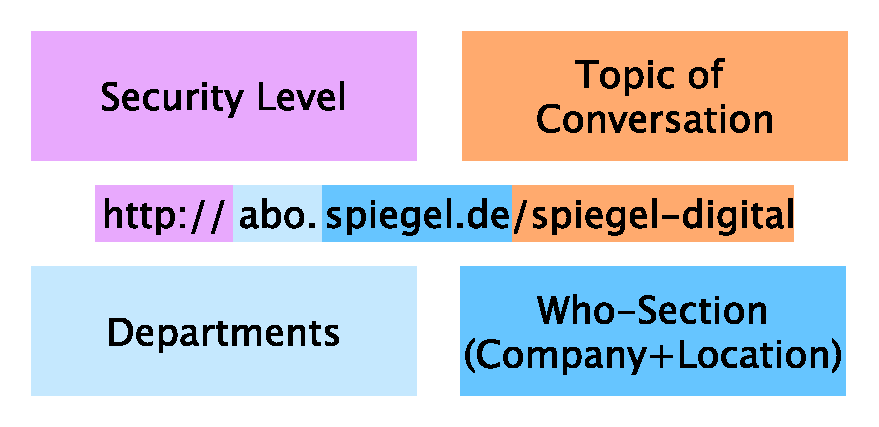
\includegraphics[width=0.56\textwidth]{url_components.pdf}
\caption{URL components that are communicated to the user}
\label{fig:url_components}
\end{figure}

\begin{figure}[hHtbp]
\centering
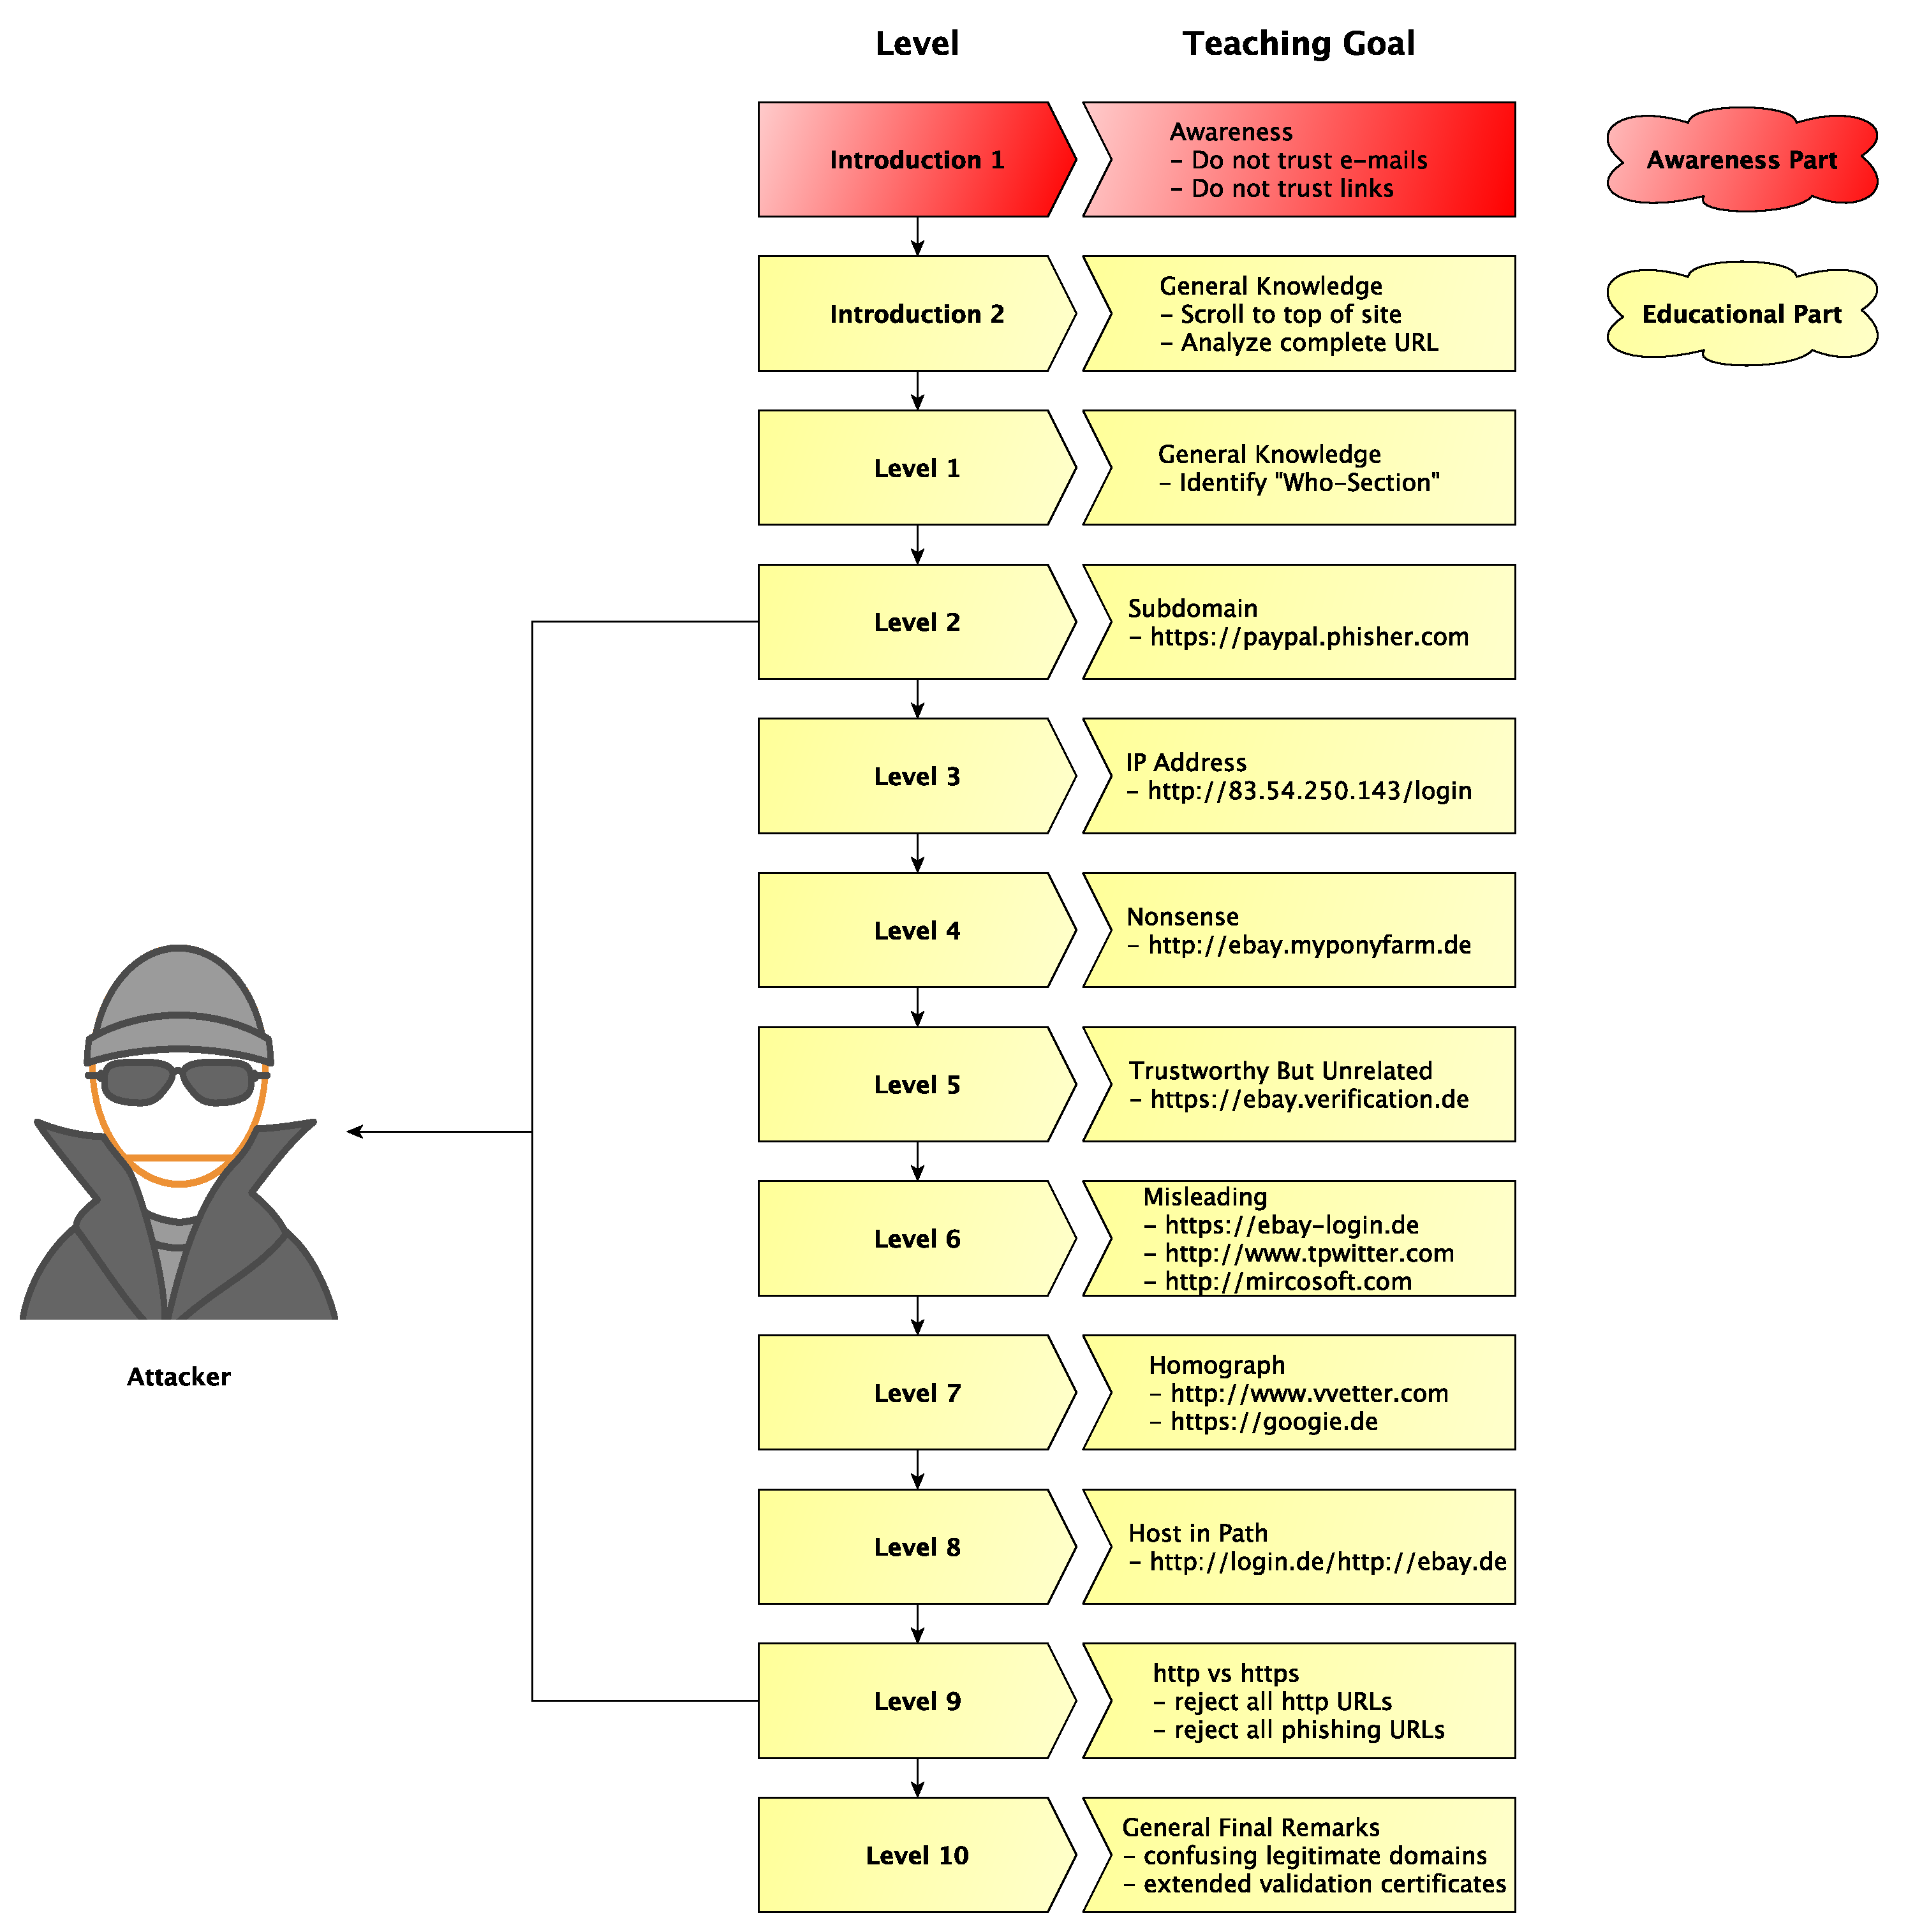
\includegraphics[width=1.0\textwidth]{graphix/level_teaching_goals.pdf}
\caption{Teaching goals per level}
\label{fig:level_teaching_goals}
\end{figure}


%===========================================
\subsection{Leveling Strategy}
\label{s:leveling}
%===========================================
During the app development we examined several strategies on how to gain points and setting thresholds for unlocking the next level and incrementally improved it.
 This section is intended to introduce the leveling strategies we considered for the app together with an assessment of their strengths and weaknesses.
Finally, we describe the strategy we chose to use.

\begin{description}[leftmargin=0cm]
	\item[Leveling Based on Achieved Points:] Our very first leveling strategy was based on the achieved points per level.
 On each level the user had to achieve 100 points to pass the current level and unlock the next one.
 This approach had a major drawback.
 The fact that achieving a minimum of points to pass the level results obviously in very similar points for everybody finishing a specific level.
 That is to say, the comparison between single users would not be meaningful as the points would only differ very slightly.
 Additionally, users gain points for each run of a level. Therefore, given the fixed amount of points to be achieved, users might replay early levels which are easier and gain the same or even more points compared to users playing later and more difficult levels.
	\item[Leveling Based on Detected Phishes:] The previously described leveling strategy had the deficit of comparability among the users.
 However, we consider comparability very important  since it serves as an incentive for the user to perform better or play on.
 For this reason, we decided that passing a level should rather depend on the number of phishes the user was able to detect during a level.
 That is to say, in every level there is a certain amount of phishes the user has to detect in order to complete it.
 With this approach there is still the possibility for a user to repeat early, and thus easy, levels and possibly gain more points than users playing later, and thus more difficult, levels.
 To prohibit this, in increasing levels the users gains and loses increasing points accordingly such that it does not pay off to replay lower levels.
 The points for each answer $p$ in each level $n$ is modified by the following formular:
 $$p*1.5^n$$
 This strategy solved the problems of our first strategy, however it also brought a new one: always rejecting a URL will eventually result in passing the level (if the user also correctly identifies the domain when required). Such a downside is suboptimal for a game.
	\item[Leveling Based on Correct Answers:] To solve the problem of our second leveling approach we extended the leveling passing to correct answers.
 Instead of detecting a certain amount of phishes per level, the user has to give correct answers to a predefined amount of phishing URLs as well as a predefined amount of valid URLs in order to pass a level.
 Only and only if the user correctly answered the predefined number of valid and phishing URLs the level is completed.
 To additionally incentivize the users we included three lives per level.
 The lives are supposed to prevent a user from playing eternally, without ever passing the current level.
 In case the user loses all of his lives, cf. \autoref{fig:lose_points_life}, this indicates that he did not understand what the level was about.
 Therefore, he has to restart the level. He is returnt to the introductory block of the level he just lost.
 The points are assigned exactly as before.
 This is our final leveling strategy for the app.
\end{description}

%===========================================
\subsection{Use of Learning Principles and Game Techniques}
%===========================================
Our app is a learning game which purposes to introduce information on the topic of phishing and how to detect it.
With the app we want to improve understanding for this topic and help users be less vulnerable for falling for such attacks in future.
This section deals with the principles of learning and game techniques which are reflected in our app design.
In fact, the laws of learning and game techniques have a strong connection which is the reason why games work for learning purposes~\cite{murphy2011games}.
%--------------------------------------------------------------------------
\subsubsection{Principles of Learning}
%--------------------------------------------------------------------------
\label{s:learning_principles}
Edward Thorndike introduced the first three principles of learning: readiness, exercise and effect~\cite{thorndike1932fundamentals, murphy2011games, handbook2008us}. 
Later the principles of learning were further extended by: primacy, intensity and recency~\cite{murphy2011games, handbook2008us}.
These principles outline how people learn and which conditions improve their process of learning.
In the following we will briefly introduce the meaning of these principles~\cite{murphy2011games} and explain how they are reflected in our app.

\begin{description}[leftmargin=0cm]
	\item[Readiness:] The principle of readiness claims that physical, mental as well as emotional preparedness is an important prerequisite for a better learning performance. 
It also states that motivation is crucial for effective learning. 
First of all, students must want to learn something, otherwise any additional motivational efforts will be of no use. 
In order to make students want to learn something it is relevant for them to see a clear reason for learning, i.e. the perceived value of the material is ultimately related to their motivation. 
Finally, the principle of readiness says that best learning performances are achieved in combination with good physical health.
The physical and health conditions of our app users are beyond our control.
For this reason this is an aspect which cannot be reflected in our app.
The app is targeted at users who are willing to learn something about phishing. 
Consequently, there is already some kind of motivation in our app users.
In order to increase this motivation we present clear reasons why the user should continue to play our app.
This is happening in the awareness part, where the user is told what exactly phishing is, how easy it is to phish users, spoof e-mail senders and content, spoof links as well as create exact copies of legitimate websites, cf. \autoref{s:app_design}.
	\item[Exercise:] The use of exercise is composed of two important parts: 
First, training and repetition help increase learning. 
Second, feedback is crucial for good learning performance.
For best learning results, these two parts must be applied together.
In a nutshell, the learning connection is strengthened by practice, and weakend by disuse~\cite{handbook2008us}.
After finishing the awareness part, we start with the user education and provide exercises for all of our learning goals (except for the last level), cf. \autoref{s:knowledgetransferperlevel}.
The learning content is also permanently repeated. 
For example, in the introduction 2, cf. \autoref{s:knowledgetransferperlevel} the user learns to scroll up to make the address bar re-appear and analyze the URL by right and left scrolling it. 
The scrolling of the URL is present in levels 2-9.
Also, the user has to identify the Who-Section in level 1. 
In addition, the user has to show the Who-Section every time he has detected a phishing URL correctly.
Finally, every introduced attack of each level n will appear in level n+1 at least once. 
That is to say, as soon as the user gets to know a new attack, he will keep seeing this attack in the succeeding levels.
Our app also provides direct feedback to the users' actions. 
In case of correct answers, the user is rewarded with gained points, with a smiley and a small text that he has done well.
When the user has made a mistake he is punished with losing points, possible life loss and a sad smiley. Also, the user is told that the answer was wrong, why it was wrong and additionally he gets a reminder text on the applied URL spoofing attack he was not able to recognize.
To sum it up, we let our app users practice what we taught them and make use of repetitions in combination with direct feedback.
	\item[Effect:] A student who associates his learning with positive feelings will learn more and better than another student who connects his learning with negative feelings. 
For example, a student who is unsuccessful with initial learning material will associate his experience with unpleasantness, frustration, anger and/or confusion, while a student with early success will have strong positive feelings and thus will be more motivated to have more success in future.
Therefore, enabling particularly early success and maintaining student motivation with positive feedback and comments is crucial.
In our app early success is easy to achieve, since we start with easy tasks and obvious attacks which get increasingly difficult in higher levels.
When the user has given a correct answer he is rewarded with a big smiley face as well as points. 
Also, the user is shown a medal every time he finishes a level.
These aspects of the app are intended to increase the users' positive feelings and keep him motivated to go on. 
However, some improvement of positive comments might be worth considering.
Currently, the positive texts for a correctly answered text, for finishing a level and icons do not differ. 
It might be more engaging if such texts and icons differ from time to time in order to increase the positive emotions of the user. 
For example, texts telling the user that he has done well might slightly vary (for instance, according to the degree of difficulty of the achieved task).
Also, the screen of finishing a level could vary.
Here again the degree of difficulty might be considered. 
According to the level finished, the obtained award could get bigger, the text of the level finished screen more flattering in order to increase the users positive experience.
	\item[Intensity:] This principle says that learning is better encouraged by things that are more intense. 
For example, people likely to learn more from an exciting and enthusiastic teacher than from a boring and monotone one or from a text book.
Our app is by nature more intense than a simple text based approach.
The game creates incentives and intensity.
Also, the fact that we do not only tell the user that e-mail spoofing and link spoofing is easy but also make him experience it increases the intensity.
	\item[Primacy:] The principle of primacy means that the first thing a student learns makes the strongest impression. 
For this reason getting rid of bad habits, and replacing incorrect or wrong logic are difficult. 
This principle is coupled with time. 
The first things our users learn is: what is phishing as well as how easy e-mail and link spoofing is. 
For those who already knew these things, the awareness part will not be such a high motivating factor. 
Yet, we believe this part is indispensable since there are still many people outside who are not aware of the aspects mentioned above. 
	\item[Recency:] The principle of recency states that most recently learned things are easier to remember. 
This is a consequence of the reduction of the learning over time. 
The principle of recency is coupled with time. 
We are aware that our app is not a game which will be frequently used and thus its users are likely to forget the content they have learned, for example, a week ago. 
In order to overcome this problem, so called reminders are included in each new level introduction.
An example view of these reminders is depicted in \autoref{fig:Screenshot_intro2.png}. 
There the user has a short summary of what he has learned so far. 
Also, we keep confronting the user with attacks from previous levels during the exercise rounds.
This repetition is, on one hand, intended to strengthen the users knowledge and understanding, on the other hand, it is intended to create a kind of recency so the user does not forget about this kind of attack. 
In case the user does not detect the attack (a repeated or a new one) he will be reminded what kind of attack had been applied. 
Furthermore, in this level the user will be confronted with this kind of attack again, until he gives a correct answer to it.
\end{description}
Now that we have introduced the fundamental principles of learning and associated these with our app, we proceed with the introduction of game techniques and how they are related to the learning principles as well as to our app. 
As already mentioned, there are strong connections between learning principles and game techniques. 
Therefore, we will try not to focus on redundant aspects, but rather on additional aspects which need to be considered in game design. 
%--------------------------------------------------------------------------
\subsubsection{Game Techniques}
%--------------------------------------------------------------------------
\label{s:game_techniques}
Basic game techniques are: flow, feedback, simplicity, immersion and engagement, choice and involvement, practice as well as fun~\cite{murphy2011games}.
As some terms already reveal, these principles are strongly connected to the basic principles of learning.
In the following we will elaborate on these game techniques by stating their relation to the according learning principle, mentioning  additional aspects to consider and how these are mirrored in our app.

\begin{description}[leftmargin=0cm]
	\item[Flow:] Flow is the key point of games. It is ``the state in which people are so involved in an activity that nothing else seems to matter; the experience itself is so enjoyable that people will do it even at great cost, for the sheer sake of doing it''~\cite{csikszentmihalyi1990flow}.
Sometimes flow is also referred to as 'engagement'~\cite{murphy2011games} and relates to a person's overall well-being~\cite{seligman2012flourish}. 
Flow relates to motivation~\cite{csikszentmihalyi1990flow, csikszentmihalyi1997finding}. Motivation in turn is a crucial part of readiness, cf. \autoref{s:learning_principles}.
In essence, there are four requirements for flow~\cite{csikszentmihalyi1990flow, csikszentmihalyi1997finding, schell2008art}.
	\begin{enumerate}
		\item \textit{Clear Tasks:} With clear tasks the user is able to understand what he needs to do. 
The tasks which need to be completed by the users of our app are never complex and they are always clearly told what they need to do next. 
		\item \textit{Feedback:} With feedback the user should always be kept up-to-date about his progression towards the goals he is asked to achieve. 
He also should get immediate feedback on whether his actions are good or not. 
Our app covers these aspects, cf. \autoref{s:learning_principles}.
		\item \textit{Balanced, Attainable Goals:} The user should be confronted with challenging tasks, but at the same time these tasks should also be achievable. 
Especially in the beginning our app users are confronted with very simple tasks.
For some users they even might be too easy which may result in a loss of interest.
However, these tasks are important basics which are necessary for successful detection of phishing attacks on the smartphone. 
Therefore, for future work especially the first two tasks (access address bar and analyze the complete URL) could be re-designed so that they also keep users which have already knowledge in this area.
Currently, the users can just skip the introductory part of this part and directly complete the task.
Besides, as the users' skills will naturally improve, their tasks get more difficult and challenging with increasing levels, but will remain achievable.
		\item \textit{Concentration:} The user should not be distracted with, for example, complex interfaces. 
He should rather be able to fully concentrate on the game. 
Our app has a very simple user interface with the most necessary elements. 
There are no special effects, advertisement or other elements which might distract the user from playing the game with full concentration.
The only intrusive and interruptive elements are our introductory sections. 
However, these are inevitable for the communication of the learning content.
	\end{enumerate}
	\item[Feedback:] Feedback is important which is also reflected by the fact that it is a crucial part of the learning principle 'exercise', cf. \autoref{s:learning_principles}, as well as a requirement for flow.
Stated simply, feedback is how a user perceives progress~\cite{csikszentmihalyi1990flow, csikszentmihalyi1997finding}.
For the completion of even simple tasks feedback is indispensable.
Feedback can be in form of a scoring system, comparative statistics or failure outcomes and provides the user information about his progression and performance.
Games make use of a so called feedback loop~\cite{goetz2011harnessing}:

\begin{enumerate}
	\item \textit{Measure Behavior:} Our app assesses whether the answer of the user to a given task is correct.
	\item \textit{Relay Measurement to User:} The user is told whether his answer is correct or not.
	\item \textit{Realize Some Sort of Outcome:} The outcome of the users' actions and answers are accordingly defined, cf. \autoref{s:game_rules}. 
For example, the user loses a life in case he did not detect a phishing URL.
	\item \textit{Provide Opportunities for Alternate Action:} 
The user has the chance to do better in the next tasks.
\end{enumerate}
	\item[Simplicity:] The real world is a complex construct.
However, games should simplify the real world so that there only remain rules and goals.
In this way the players can fully concentrate on their tasks and how they can achieve them~\cite{csikszentmihalyi1997finding}.
Hence, simplicity helps users to achieve flow and thus increased motivation. 
This, in turn, leads to improved learning, cf. \autoref{s:learning_principles}.
Simplicity involves, for example, the user interface, the game goals, feedback loops, rules and instructions.
The structure of our app is kept simple and consistent.
Therefore, it should be easy to understand.
Our user interface is kept to the necessary minimum and the goal of the game is clear: detect phishing URLs.
	\item[Immersion and Engagement:] Immersion involves a passive activity. 
The term is used, for example, to describe a person who shows strong interest for a story~\cite{mcmahan2003immersion}. 
In contrast to immersion, engagement involves active actions, such as trying to solve a problem or puzzle.
Games commonly use both, immersion and engagement.
To achieve immersion game designers make use of stories, visual and audio techniques, attractive graphics or animations~\cite{schell2008art}.
Simultaneously, the user is engaged with choices, problems, or puzzles which have to be solved.
The combination of immersion and engagement has the potential of creating an intense game experience~\cite{murphy2011games}.
These two aspects of game techniques are strongly linked to the learning principle of intensity.
By challenging the user with various tasks to solve we meet the requirement for achieving engagement. 
However, immersion is an aspect we have not considered yet within the scope of this thesis.
In order to achieve an intense game experience, this aspect might be worth considering for future work.
	\item[Choice and Involvement:]
Games consist of choices and involvement. 
There is a link between choice and positive feelings (cf.~Principle~of~Effect~in~\autoref{s:learning_principles}), i.e. choice is important for a person's overall well-being~\cite{seligman2012flourish, schwartz2009paradox}.
However, the downside of choices is the so called paradox of choice which states that choice is beneficial, but too many choices can cause more bad than good~\cite{schwartz2009paradox}.
The problem is, when the users are confronted with too many choices they get overwhelmed, since the decision thus the task to solve becomes too complex.
We believe that our app does not face the problem of this paradox since the decisions the user has to take are limited to the questions:
is the following URL a phish, and show us the Who-Section.
Still, the user has to make decisions and is consequently involved in the game.
	\item[Practice:] This technique is directly related to the learning principle of exercise, cf. \autoref{s:learning_principles}. 
Users practice and repeat several steps of games extensively so that they eventually gain mastery and the difficulty of their challenges can increase\~cite{murphy2011games,schell2008art}. 
Our app offers practices as well as repetition, cf. \autoref{s:learning_principles}.
	\item[Fun:] Fun is an important aspect of game design and yet the definition of it is not clearcut in literature~\cite{murphy2011games, schell2008art,koster2010theory}.
Based on several definitions found in literature Curtiss Murphy introduced the following definition of fun: \textit{``Fun is the positive feelings that occur before, during, and after a compelling flow experience''}~\cite{murphy2011games}.
Positive feelings include, but are not limited to, engagement, enjoyment, pleasure, entertainment, satisfaction, control and triumph. 
Fun is related to the learning principle of effect and its positive feelings.
How we achieve the principle of effect and positive feelings in our app is described in \autoref{s:learning_principles}.
Yet, fun is something which emerges from several game techniques, such as, flow, immersion and engagement, practice to achieve mastery, and choices, which all lead to positive emotions.
Fun is an aspect of our app which could be considered more deeply in future work. 
Especially, the areas of creating positive feelings and including immersion in order to make the users' game experience more intense and fun are aspects which might be looked at.
\end{description}
	
%===========================================
\section{Development Process}
%===========================================
This chapter summarizes important steps concerning the development process of our app.
We do not provide in-depth insight to our source code. 
Instead we give a brief overview of our approach for the development of a user friendly and understandable app.
%===========================================
\subsection{Mock Up}
%===========================================
After we decided about the work flow and structure of our app we built a mock up in order to get a more concrete idea of what needs to be implemented and to reveal flaws in our thought process.
We showed it to friends and relatives so we could expose aspects we have not yet thought about.
The first texts explaining how to access the address bar and the structure of a URL seemed to be difficult to understand.
As a consequence, we adjusted these texts in the app (only those of the first three levels) and showed them to other friends and relatives who seemed to understand the descriptions.
Based on these initial texts we wrote all remaining texts without including it into the app yet.
The next section describes the elaboration process of these texts.
%===========================================
\subsection{Pilot Study of App Texts}
%===========================================
\label{s:pilot_study}
After finishing the texts for each step of the app flow (the texts were not directly included into the app) our supervisor, a professor of pedagogy at TU Darmstadt as well as another highschool teacher of German reviewed them.
Once we achieved the version with which we were satisfied we applied a user study on it. 
For time reasons, we decided to go for the low cost method of guerilla user testing~\cite{guerillagovuk, guerillauxbooth}.
This approach enables to quickly assess the effectivity of a design, in our case our app texts.
Guerilla user tests is rather loosely structured and do not include participant recruitment.
The testers are rather approached, in our case, we asked relatives and friends. 
The outcome of such studies is rather qualitative, i.e. extensive and detailed insights are achieved.
A downside of guerilla testing is that the approached participants might not belong to the defined target group with respect to their expertise or skills. 
Since we knew our participants we addressed only those who matched our target audience. 
In detail, our approach for the guerilla user test was as follows:

\begin{enumerate}
	\item\textit{Preparation of Texts:} Our aim for this user test was to imitate the use of a smartphone as best as possible.
	For this reason, the app texts were formatted into short lines, so that the text appearance resembled that of a smartphone screen.
	Furthermore, we printed out the texts and cut the sheets into small rectangles.
	\item\textit{Think Aloud:} We asked the participants to think aloud during the test. 
	We told them that there are no stupid questions or comments and that they help most with just saying what goes through their mind.
	We made notes of their remarks.
	\item\textit{User Test with In-Between Exercises:} The actual user test mainly consisted of reading our app texts and thinking aloud about these.
	We included a little simulation of our exercise parts in order to validate whether the users comprehended the texts or not.
	For example, for each introduced attack we included a small list of URLs on which the users had to decide whether they were phishing URLs or not.
	\item\textit{Final Comments:} After going through the texts the users were asked to provide their general impression.
	We further asked them about some aspects we were not quite sure about at the beginning. 
	For example, we asked them whether the usage of the terms ``link'' or ``web address'' confused them, which was not the case.
\end{enumerate}
Our guerilla user tests showed that our texts are understandable.
According to our participants the main downside of the texts was their length. 
Yet, this can be neglected since the users had to read our complete texts (instead of for example just playing 1-2 levels at once). 
Furthermore, they remarked that the introduction on how to access the whole address bar and analyze the complete URL is unnecessary. 
For some users this might apply. 
However, it is possible that there are users who do not know this. 
For those who already know how to access the address bar and analyze the complete URL we added a button which directly links to the exercise. 
In case the user had overestimated himself, he will be forwarded back to the app, where the introductory text can be consulted. 
Finally, the provided brief summary of already passed lessons (reminder texts) received some criticism for their frequent re-appearance at the beginning of each level. 
This can also be neglected since we assume that our app users will not constantly play this game and in our view repetitive serving of the major lessons learnt is helpful to internalize them (cf. Principle of Exercise in \autoref{s:learning_principles}). 
Also, when playing the app this screen can easily be skipped as it exhibits a recognition value achieved by the title ``reminder''. 
Moreover, we decided for a minor reorganization of the reminder view. 
Before the user tests the reminders mainly referred to the URL structuring they have learnt so far. 
We thought it is also important to remind the users of possible attacks. 
Therefore, the reminder concerning the URL structure was kept to a minimum with the aid of a graphic. 
Plus, for each attack in previous levels one sentence and one example was added.  
To sum it up, the introductory blocks that introduce spoofing techniques of phishers (level 2-9) are generally structured as follows:
First, we provide the major lessons learnt from the previous levels in the reminder.
An example reminder view of level 3 is depicted in  cf. \autoref{fig:Screenshot_intro2}.
Next, a brief introduction to the current level's topic follows.
Finally, the new attack is introduced which includes one or more examples.
An example of this view is shown in \autoref{fig:Screenshot_intro3}.

\begin{figure}[hHtbp]
\centering
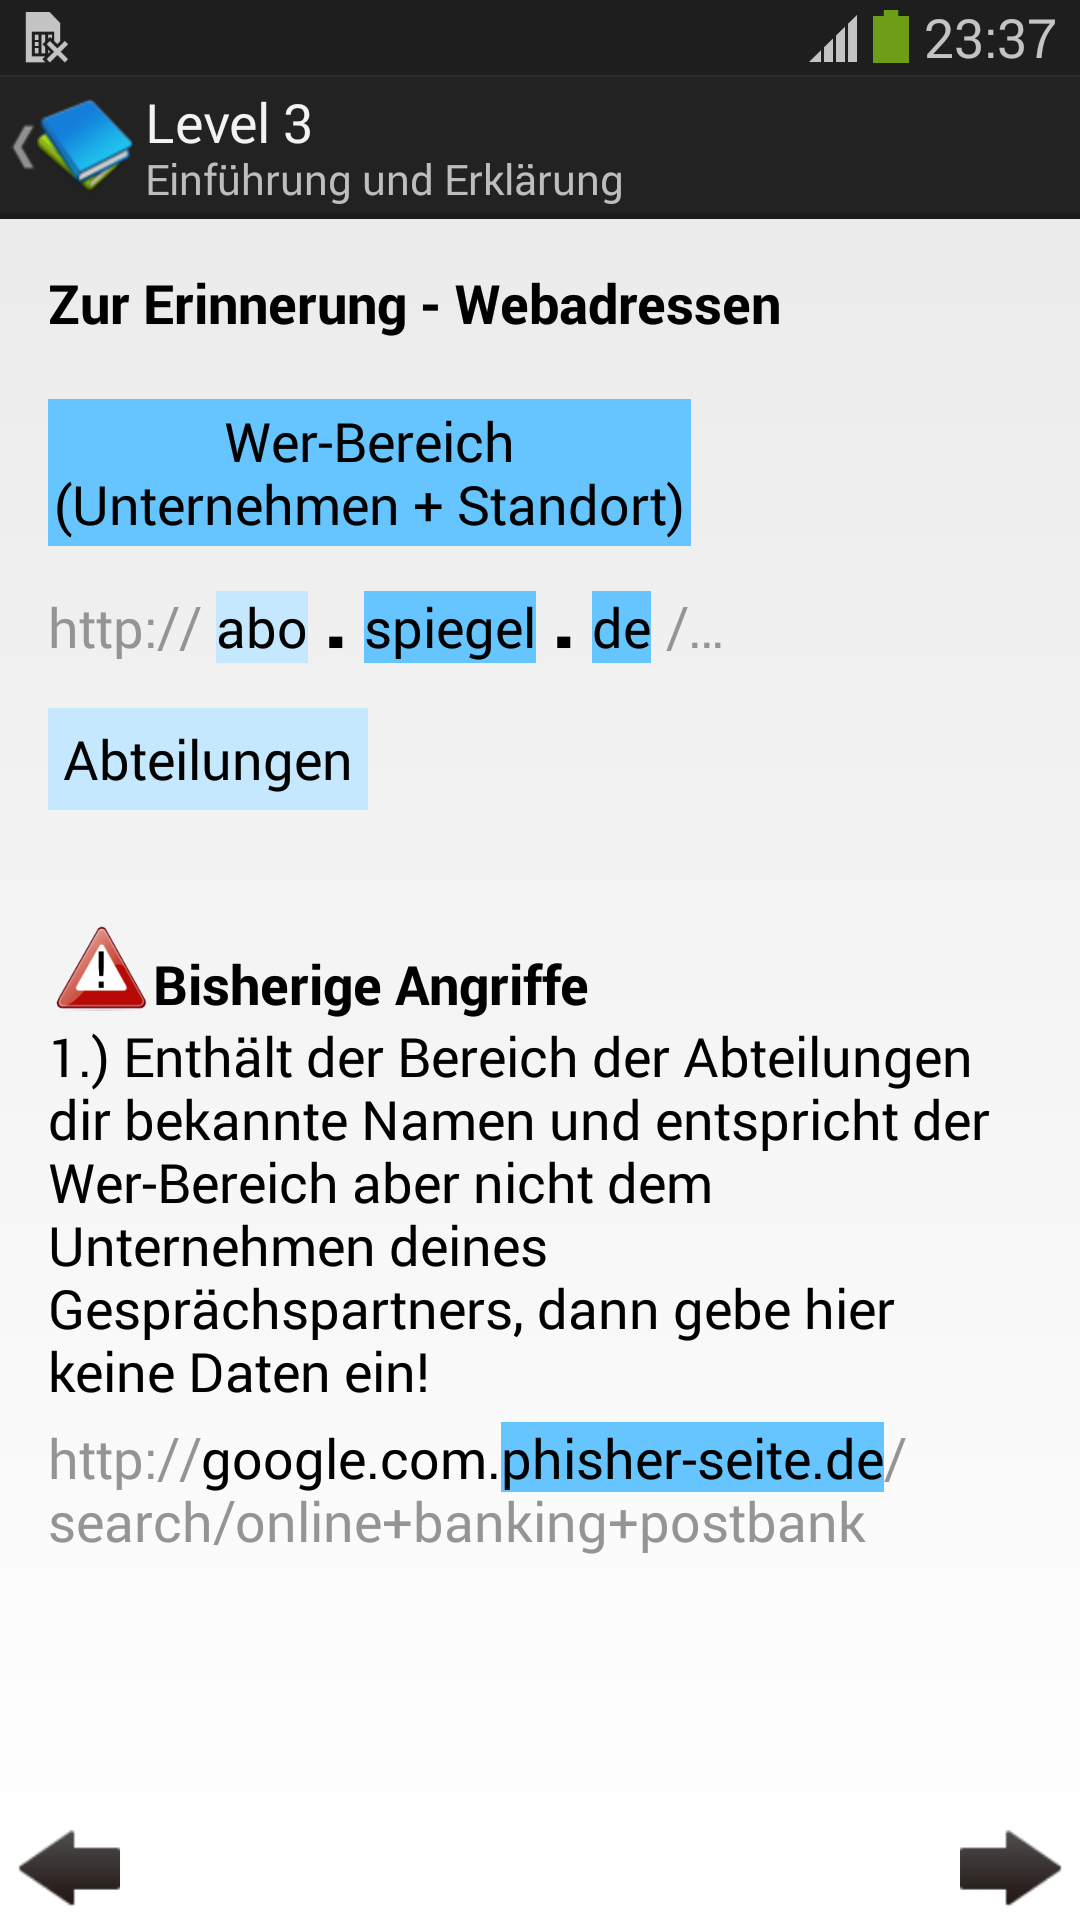
\includegraphics[width=0.4\textwidth]{Screenshot_intro2.png}
\caption{Example reminder view of level 3}
\label{fig:Screenshot_intro2}
\end{figure}


\begin{figure}[hHtbp]
\centering
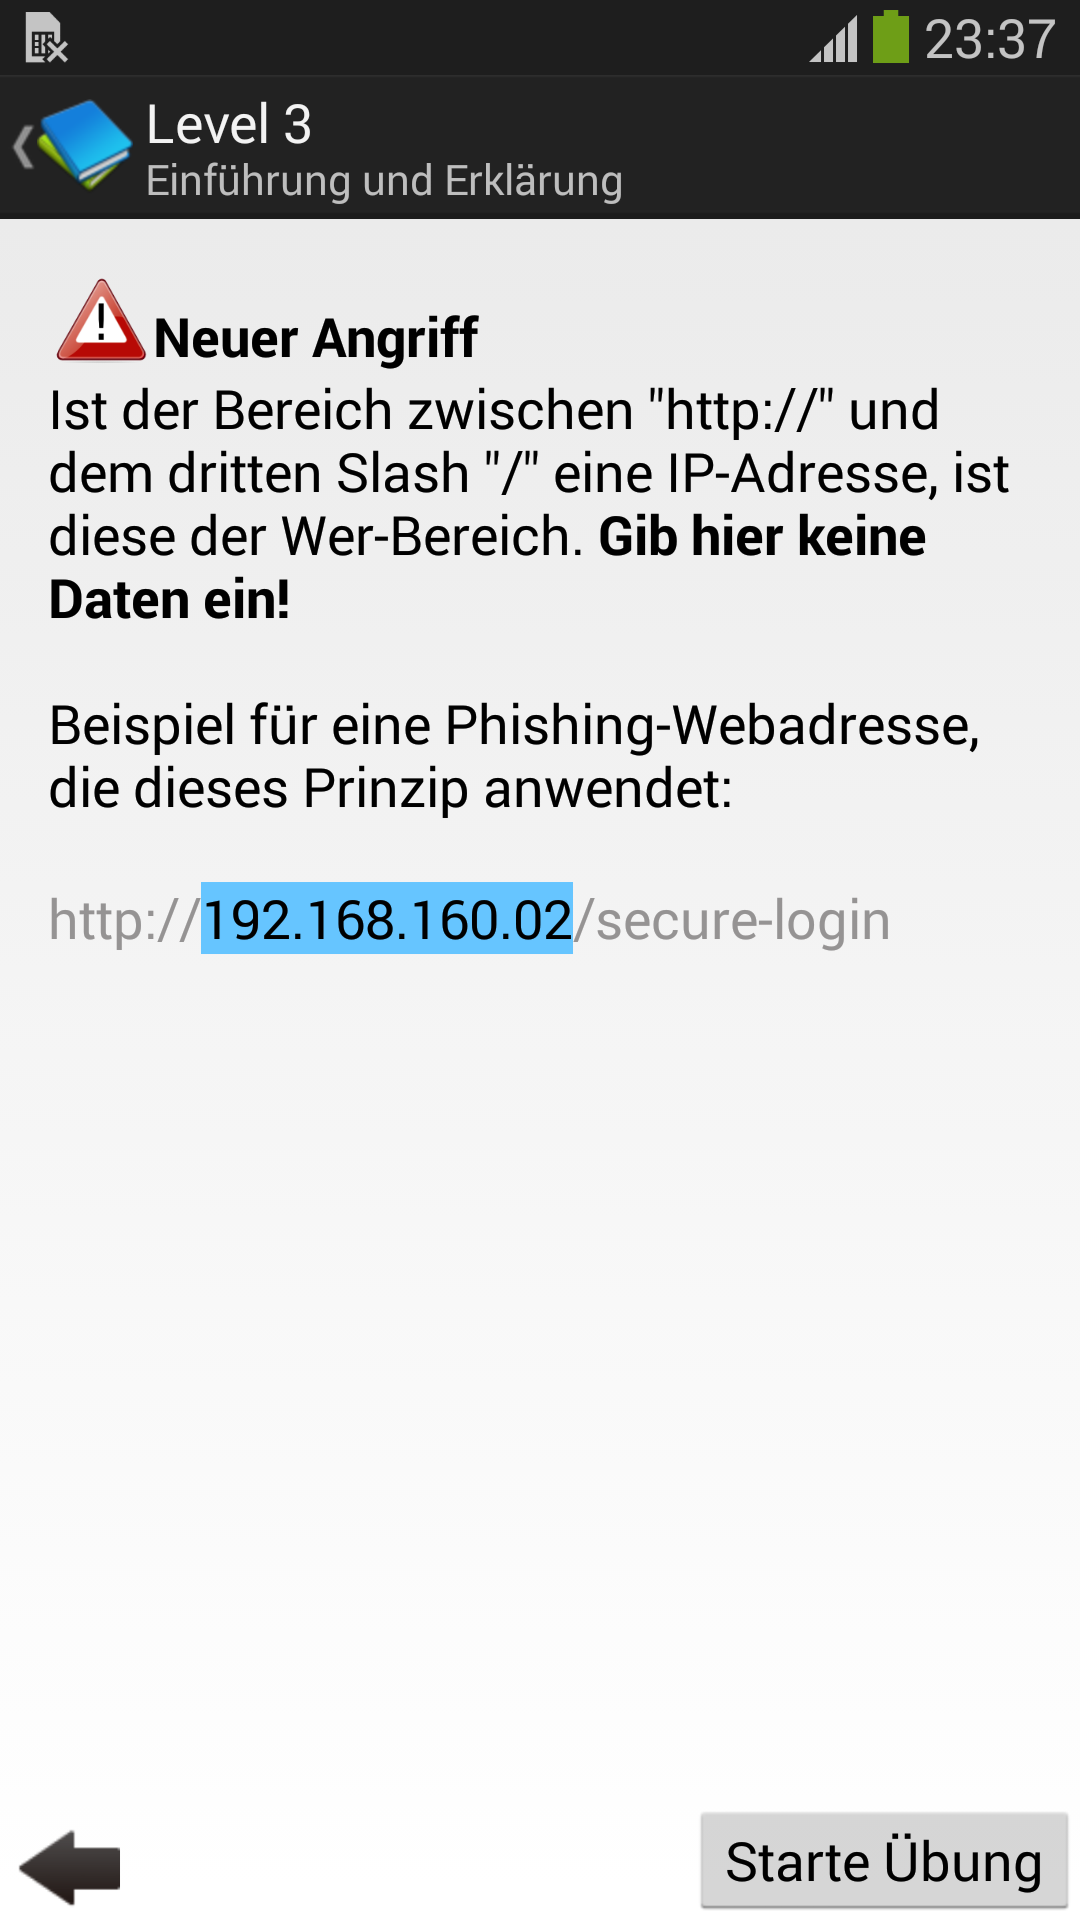
\includegraphics[width=0.4\textwidth]{Screenshot_intro3.png}
\caption{Example view of new attack in level 3}
\label{fig:Screenshot_intro3}
\end{figure}

\subsection{Implementation and Testing}
In parallel to formulating and validating our app texts we developed the basic structure and logic of our app.
After conducting and assessing the guerilla user tests of our texts and integrating the feedback, we started to include them into our app.
We both developed and tested the app simultanously.
Occasionally, we showed the app to friends and relatives in order to get some feedback on aspects we might have missed.
In this way, our app was formed incrementally. 
We do not intend to provide implementation details in this work.
The only exception is the algorithm used to generate the URLs on which the users have to decide whether they are phishing URLs or not. This approach can be consulted in \autoref{s:url_generation}.

	%*******************************************
\section{Evaluation}
%*******************************************
\label{s:evaluation}
\textbf{VLL FORMS IN APPENDIX? }As a final step the Anti-Phishing Education we have designed and implemented needs to be evaluated which is the goal of this chapter.
 The app will be evaluated with the aid of a user study.
 After introducing our study design, we will state our hypothesis and explain how we are going to measure our statements in order to prove that they are true or false.
 Finally, we will analyze our results and state our conclusion.


===========================================
\subsection{Participant Recruitment}
===========================================
%Oder was soll hier rein? ;)
%osn - freundes freunde
%telefon -freundes freunde
%flyer ausgeteilt
%flyer per e-mail an sehr viele professoren geschickt und gebeten weiter an studenten zu leiten
%ein paar leute auf der straße angesprochen - da erfolglos
%Verlosung eines amazin gutscheins


%===========================================
\subsection{Study Design}
%===========================================
For time reasons and lack of participants we decided to run a "Before and After App" Study with the same groups of people.
 Specifically, our user study is structured as follows:

\begin{enumerate}
	\item \textbf{General Before-Survey} At the beginning the participants have to fill out a general survey, where they have to judge their own knowledge on the topic of Internet security in general.
 For instance, they are asked whether it is easy for them to distinguish legitimate e-mails and websites from fake ones.

	\item \textbf{Website-Survery Before} In this part of the user study the participants gets a list of screenshots of websites.
 The screenshots had been taken with the standard browser of an Android tablet.
 In total, the user is shown 16 screenshots, with 8 phishing and 8 valid URLs.
 The user has to decide whether he would enter confidential data on the shown website.
 Additionally, he has to encircle the part of the screenshot which was the primary reason for his decision.
 Then, the user has to indicate how sure he was about his answers on a Likert scale.
 Finally, the user is asked whether he knows the vendor of the website and whether he has a account there.

	\item \textbf{Play App} After the "Website-Survey Before" the users get the smartphones in order to play the app.
 To save time, we skipped the introduction 2 part ("access address bar") for the user study.
 The user has half an hour to play the app.
 After half an hour they are asked to put the smartphones aside.
 Then, we collect the smartphones and note the reached points in each level.

	\item \textbf{Website-Survery After} After playing the app, the participants get a second website-survey.
 In this, all examples of the previous survey are included.
 Moreover, it contains 8 further website screenshots of which 4 have phishing and the remaining 4 have valid URLs.

	\item \textbf{General After-Survey} Finally, the participants are asked to fill out a form with questions to their demographics.
 This form does also contain questions related to the SUS and some other questions regarding their impression of the app.



\end{enumerate}

%===========================================
\subsection{Hypotheses}
%===========================================
In order to evaluate the effectiveness and usability of our app we have formulated the following hypotheses for the user study:

\begin{enumerate}
	\item \textbf{Hypothesis 1 - Mistakes} After playing the app, the users make significantly less mistakes in detecting phishing websites compared to before playing the app.

	\item \textbf{Hypothesis 2 - URL Based Decision} After playing the app, the users base their primary decision on whether a website is a phishing website or not significantly more often based on the URL compared to before playing the app.

	\item \textbf{Hypothesis 3 - URL Comprehension} After playing the app the user understands the importance of the second- and top-level domain of a URL as the only criteria to detect phishing websites.

	\item \textbf{Hypothesis 4 - Good Usability} The app is easy to understand and to use.

\end{enumerate}


%===========================================
\subsection{Measurement}
%===========================================
In the following we will elaborate on how we are going to measure the statements of our hypothesis and show that they are true or false.


\begin{enumerate}
	\item \textbf{Hypothesis 1 - Mistakes} Correct answers in "Website-Survery After" $>>$ correct answers in "Website-Survery Before" 
	\item \textbf{Hypothesis 2 - URL Based Decision} Number of URL markings in "Website-Survery After" $>>$ number of URL markings in "Website-Survery Before" 
	\item \textbf{Hypothesis 3 - URL Comprehension} Number of marked second- and/or top-level domains of URLs in "Website-Survery After"  $>>$ number of marked second- and/or top-level domains of URLs in "Website-Survery Before" 
	\item \textbf{Hypothesis 4 - Good Usability} System Usability Scale (SUS) $>$ 68
\end{enumerate}

%===========================================
\subsection{Results and Analysis}
%===========================================
\subsubsection{interpretation problems}
\label{s:intprobs}

\subsubsection{Analysis of our hypotheses}
\label{s:hypanalysis}

\begin{figure}
\centering
\subfigure[Before]{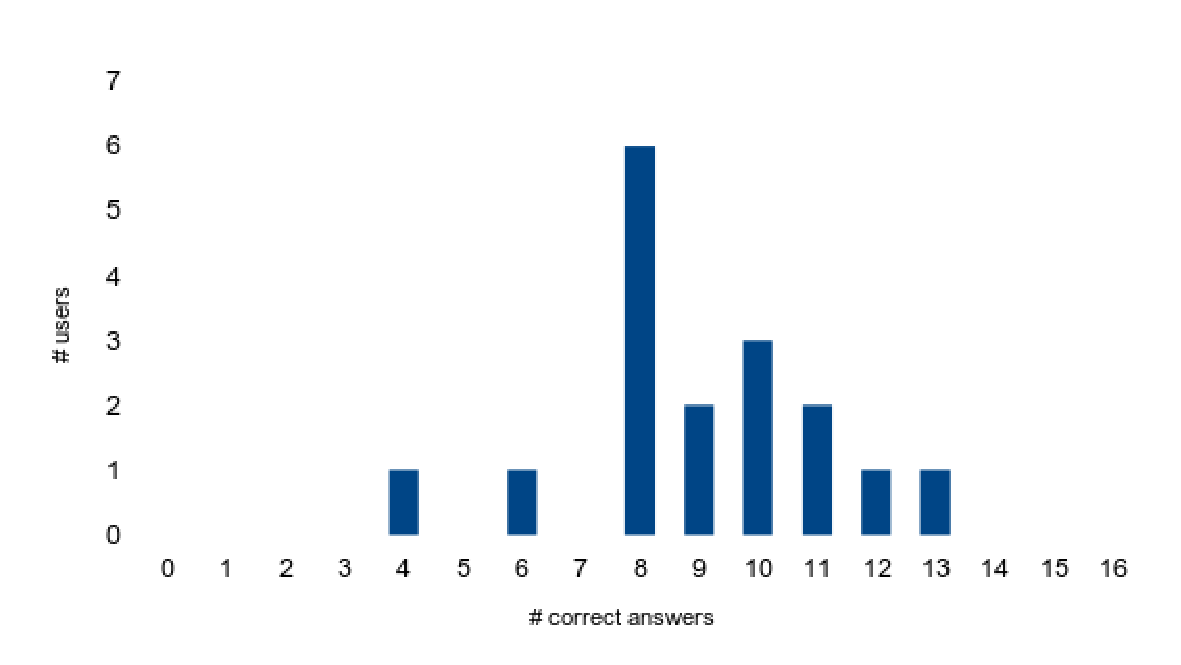
\includegraphics[width=0.45\textwidth]{hyp1b.pdf}}
\subfigure[After (all URLs)]{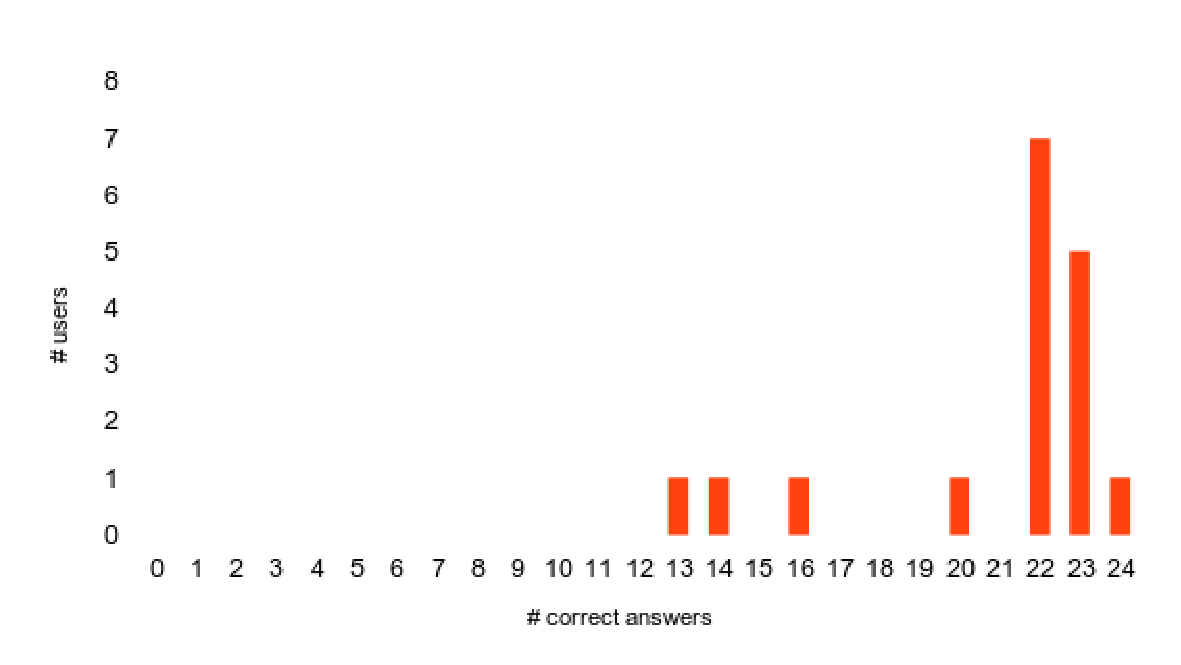
\includegraphics[width=0.45\textwidth]{hyp1a.pdf}}
\subfigure[After (New URLs)]{\label{fig:hyp1resultsanew}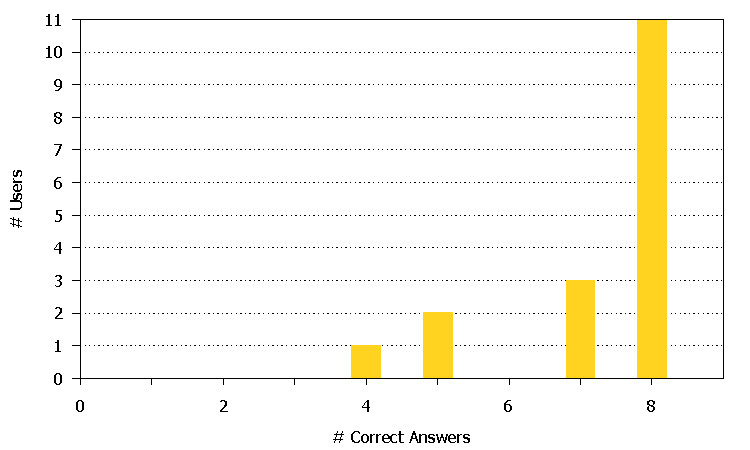
\includegraphics[width=0.45\textwidth]{hyp1anew.pdf}}
\subfigure[After (Repeated URLs)]{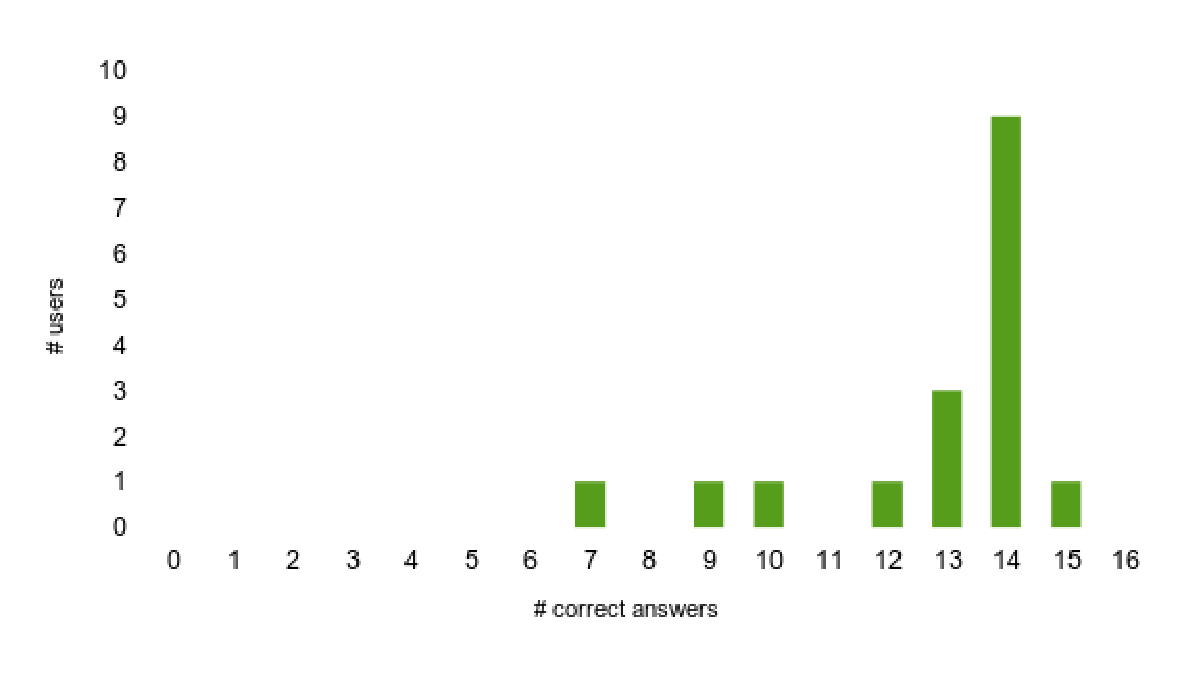
\includegraphics[width=0.45\textwidth]{hyp1arepeat.pdf}}
\caption{Correct Answers}
\label{fig:hyp1results}
\end{figure}

\begin{figure}
\centering
\subfigure[Before]{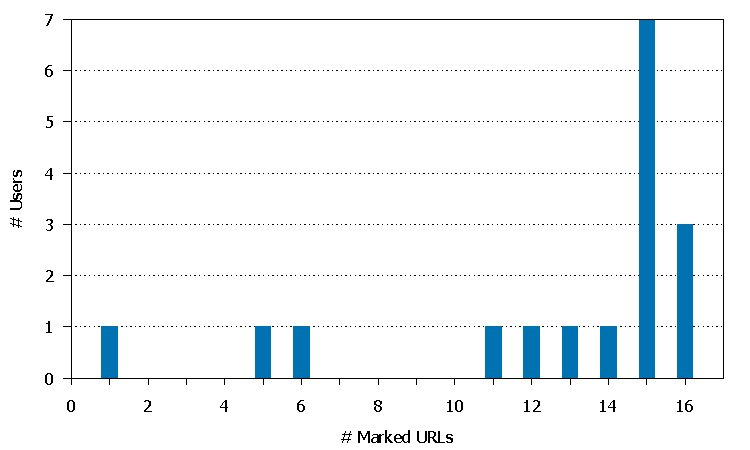
\includegraphics[width=0.45\textwidth]{hyp2b.pdf}}
\subfigure[After]{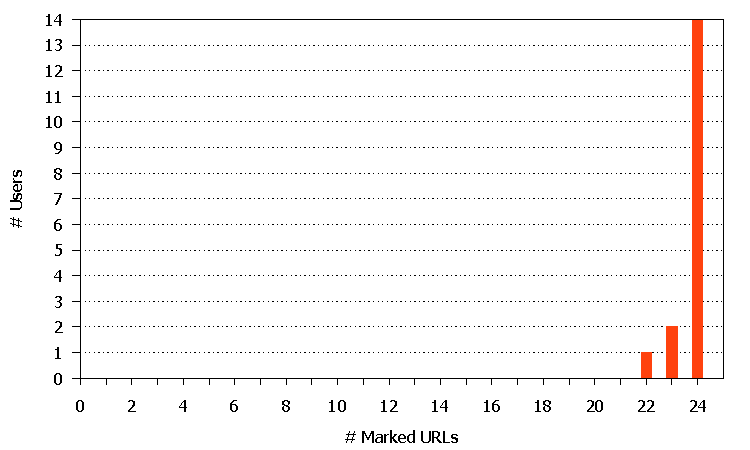
\includegraphics[width=0.45\textwidth]{hyp2a.pdf}}
\caption{URL marked}
\label{fig:hyp2results}
\end{figure}

\begin{figure}
\centering
\subfigure[Before]{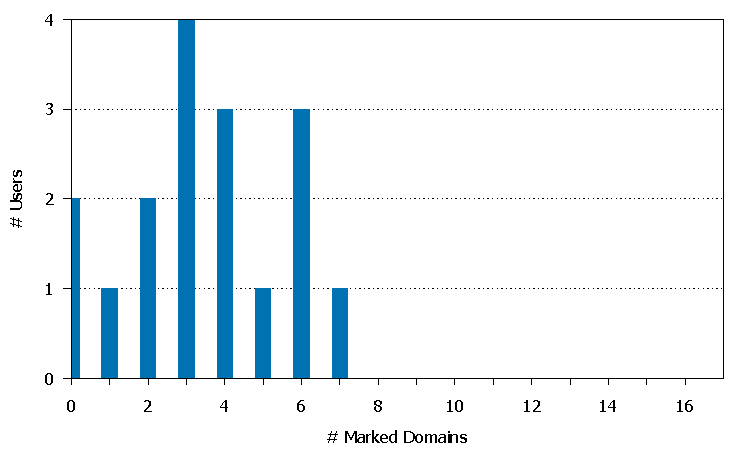
\includegraphics[width=0.45\textwidth]{hyp3b.pdf}}
\subfigure[After]{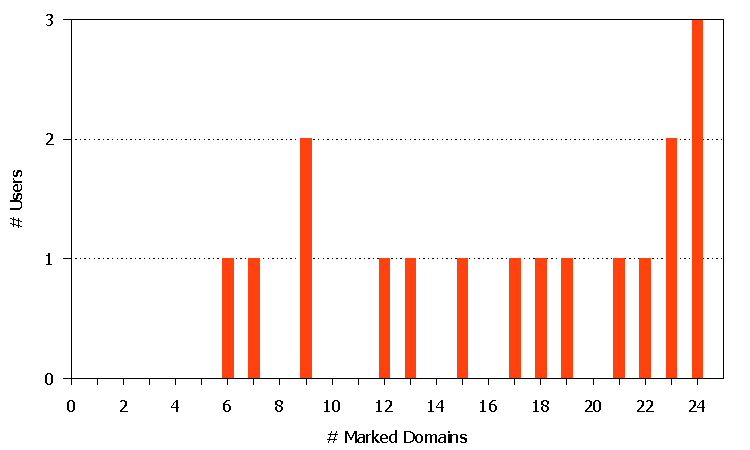
\includegraphics[width=0.45\textwidth]{hyp3a.pdf}}
\caption{Domain marked}
\label{fig:hyp3results}
\end{figure}

\begin{description}
\item[Hypothesis 1]
\autoref{fig:hyp1results} shows the results of our study according to hypothesis 1. One can clearly see that the majority of the users identified more URLS correctly after using the app than before. While most participants correctly identified 8 out of 16, i.e. 50\%, websites before they played the app, the majority gave correct answers to 22 out of 24 websites afterwards, i.e. 91.67\%. One could argue that this increase is based on the fact that the examples are mainly the same. \autoref{fig:hyp1resultsanew} however shows that the user also got most of the new URLs right. Therefore we assume that we can furthermore ignore this learning effect. 
\item[Hypothesis 2]
\autoref{fig:hyp2results} shows how many users marked the URL as their main source of decision.
Most of the users already based most of their decisions on the URL before.
Occasionally users marked the content or the padlock.
However only 3 Users (17.65\%) always marked the URL.
Afterwards we see that most users (82.35\%) always based the decision on the URL and only 3 Users made on or two mistakes.
Therefore we think that our app emphasized their believe in basing their decision on the URL.
We however think it is important to tell the user this to get uncertain or unknowing users to the same level as most of our participants.
Also our app empathizes the importance of the URL by putting the main focus on it.
We have decided against doing statistical test on this hypothesis.
We believe it will most likely be rejected because the change from before to after is not very high.
\item[Hypothesis 3]
There is a general problem with the question in the websites-before-survey.
We were not able to clearly ask the user to mark the Domain when it was the base of their decision because we would have then primed them to look at the URL or even the Domain.
This would have influenced the results of Hypothesis 2.
Therefore a user might mark the whole URL even if his decision was based only a small part (e.g. the Domain) of the URL.
We where aware of this problem beforehand but saw no other option than to formulate the question in such an open form.
Because of this we can not clearly identify what their main source of decision was in the before survey.
Afterwards the user knew that we wanted them to mark the domain.
This can be interpreted as a change of question even if the literal question did not change.
Therefore we can not apply any statistical tests on this Hypothesis.
Nevertheless none of the users marked the domain in most cases beforehand, i.e. 7 domains out of 16 URLs where marked at most by only one user.
\begin{figure}
\centering
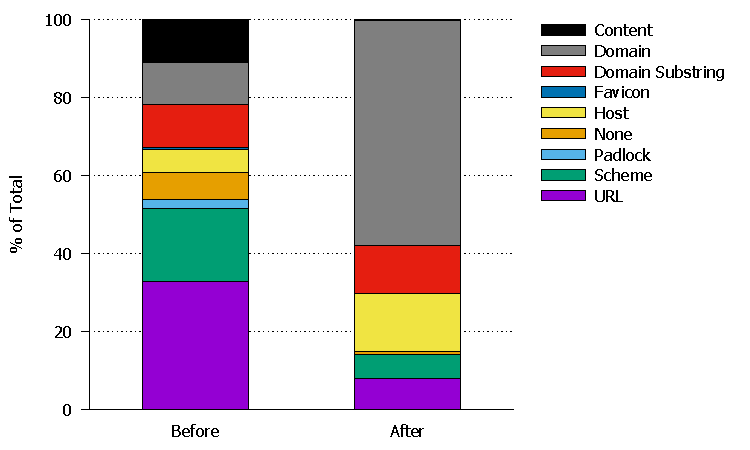
\includegraphics[width=0.45\textwidth]{markings.pdf}
\caption{Marked parts of the screenshot before and after.}
\label{fig:markings}
\end{figure}
\autoref{fig:markings} shows the distribution of the marked areas before and after. One can clearly see that afterwards most of the users marked the domain. However we are not able to compare that to the before values because of the changed question.
\item[Hypothesis 4]
\end{description}


\subsubsection{Further Exploration}
Some of the results can not be proven statistically, mainly because of the low sample count. 
Therefore, we only exploratively analyze these results in this section.
textbf{In this section we consider all of our participants. do we????} 

\begin{description}[leftmargin=0cm]
	\item[text]
\end{description}


During playing the app, the participants had a slip of paper for notes they wanted to make considering the app.
In the following we outline the main results of these slips of paper.
Note that we did not ask the users to write down something specific. 
We merely asked them to write down what they thought, i.e. there might be more participants who agreed with some of these points below but just have not explicitly written it down.
\textbf{Wenn nicht oben, dann hier auf jeden fall alle betrachten}.

\begin{description}[leftmargin=0cm]	
	\item[Scrolling of URL] In addition to deciding whether a URL is a phish or not, the user has to face two more 	challenges. 
First, the font size gets increasingly smaller in higher levels, until it eventually is approximately the same size of the Android standard browser.
Second, the URL is displayed in a horizontal scrollbar so that he has to scroll the URL to the right in order to view the beginning of it, just like it is the case in browsers.
4 of our 19 participants (21\%) found this disturbing and said it hindered them from analyzing the URL reasonably. 
Well, this is exactly what we wanted, since the behavior in the browser is the same, and users should practice it.
We assume that the users would not have noted this in this extent in case they would have had to complete introduction 2 (access the address bar), because then they would have understood why we do the URL scrolling.
Yet, we think after a couple of levels the users should have understood that they have to scroll the URL, in the game as well as in the browser, so one might consider to eliminate after some time. 
	\item[Unknown Services] We have mentioned the problem of unknown services in \autoref{s:problems_with_URLs}.
As we were afraid there are in fact services which are not familiar to several users.
4 out of 19 participants (21\%) mentioned this problem.
Even if we tried to make use of the most popular services with the aid of Alexa's~\cite{alexa} ranking we cannot assure that all used URLs are known by all users.
One idea to approach this challenge might be to provide an question mark button in addition to the check mark (no phish) and cross mark (phish) buttons. 
When a player clicks on this button, he can be told whether the given URL is a phish or not and why.
From this action the user would neither profit nor would he lose any points or lives.
Yet, we do not think that this is a major issue, since the users got at least until level 4 and most of them achieved even higher levels.
We are confident that the app in its current state is already implicitly able to teach the users about the legitimacy of unknown services.
After facing unfamiliar URLs and making or not making mistakes they will eventually learn whether to trust a service or not.
	\item[Question to Data Entry] Originally, the website-surveys before and after asked the participants whether they thought a given website screenshot was a phishing website or not.
After our test iteration of our study, however, we decided to change the question towards asking the user whether they would enter their personal data into this website in order to create some context for the user. 
As we told the user that this study was particularly about phishing and that their task was to detect phishing websites in the website-surveys before and after, we believe that it was clear what we were asking for with this question.
Yet, 3 participants (15.8\%) noted that the formulation of this question was unclear, i.e. there might have been participants who selected ``no'' even if they did not think it was a phishing website, but they would  generally not enter their data in this website.
	\item[Explanations and Comprehensibility]
4 participants (21\%) stated on their slips of paper that they found the explanations of the app very good and easy to understand.
1 of these 4 participants, however, added that there is partially much text to read.
Another participant (not under those 4) noted that there is too much and long text in general.
	\item[App Structure]
We did our best to develop an app which is consistent and well-structured.
3 of our participants (15.8\%) confirmed our intentions by stating that they found our app well and clearly-structured.
	\item[Button Positioning] The positioning of our app buttons during the game are as follows: 
The left bottom corner has a check mark which represents that the user thinks the displayed URL is not a phish.
The right bottom corner has a cross mark which means that the user thinks the displayed URL is a phish.
After clicking on either of these buttons in the write bottom corner another button appears (where the cross mark usually is) which either is the continue or the verify button (depending on whether the user has to select the Who-Section or not).
2 of our participants (10.5\%) indicated that the positioning of the buttons in the right bottom corner are suboptimal.
The problem here is that accidentally double clicking, for example, the continue button in the right corner results in rejecting the next URL even if the user might not have intended to.
Even if only 2 participants explicitly criticized this aspect we believe that this is a legitimate point.
In fact, the positioning of the two buttons continue and verify should be different from the one of the cross mark.
This is an aspect which should be targeted in future work. 
	\item[Repetition]
Repetition is an important element of our app.
In every level introduction we briefly repeat the so far learnt parts of a URL (with a graphic) and the different attacks the user has seen until this point.
We also make use of repetitions during the exercise rounds, every level contains at least one exercise from the previous level.
2 of our participants (10.5\%) explicitly indicated that our repetitions made them feel more confident and safer.
	\item[External Links]
In the main menu of our app we have a button ``More About Phishing'' which leads to a list of external links to various websites about phishing.
As it is often easier to find websites on a specific topic in English, some of these websites are in English as well.
2 participants (10.5\%) indicated that they did not like it to be led to an English website and would have expected to be forwarded on a German one.
This aspect is also a point which is worth to consider for future work, since we cannot expect our audience to have knowledge of the English language.
An idea to approach this might be to provide in-app additional info.
That is, instead of linking to external websites, the app itself could provide additional categorized information in German.
This would solve the problem with the language and at the same time the additional information would fit to our app layout and design.
	\item[Amount of Examples] Our app starts with a small sample of URLs users have to decide on.
In every level the sample size increases as the number of possible attacks increase.
2 participants (10.5\%) found that our sample size was to big.
This might have been the result of the fact that the users had to play the game for half an hour at a time.
Yet, re-thinking the number of URLs per level might be reasonable, but one has to consider that there have to be enough phishing URLs for the repetition as well as the new attack in each level.
	\item[Mail Not Received] The first part of our app includes sending a spoofed e-mail to oneself in order to increase the awareness of how easy faking e-mails is, even for unexperienced users.
1 participant did not receive the e-mail he tried to send to himself.
He skipped this part by clicking on the according button we had added for such cases.
All other participants received the spoofed e-mail.
	\item[Further Suggestions] In their notes some users made several suggestions which we found interesting and would like to mention here.
2 participants stated that the attacks in level 2 are not very challenging and very obvious.
Phishing URLs are of the following kind in this level: ``http://www.ebay.de.phisher.com/login''.
We had done this intentionally, however maybe the app could in fact start with for example nonsense attacks or just reduce the number of samples in this level.

Another participant noted that the repeating sentences ``Very good. You are now a bit safer'', for example, when the user correctly identified a phish, were kind of repetitive and not motivating enough. This is ultimately related to our issue with the Law~of~Effect in \autoref{s:learning_principles}.
There we stated that the texts and icons of the app should vary according to the user's performance and the degree of difficulty in order to achieve higher and better positive feelings.
This is an additional point which is worth to consider for future work.

A participant would have wished more ``feedback'' on his progress in general. 
He missed statistics, highscores or other forms of long-term feedback.
As we mentioned in \autoref{s:learning_principles} and \autoref{s:game_techniques} feedback is essential for learning as well as games.
For this reason, this aspect is something which should be enhanced in future.

A further interesting point is that one of our participants noted that he thought our app was appropriate for schools.
From this we infer that the participant found our app easy to understand and that he thought pupils were capable of understanding and playing our app.
In fact, this is a very good and important point.
People might not want to learn about phishing on their own, especially pupils would probably not think about that.
However, if computer security is a part of the education plan and if pupils have to learn something about, for example, phishing by playing the app, a far larger audience can be reached and educated on this topic.	
\end{description}
%===========================================
\subsection{Discussion}
%===========================================
%===========================================
\subsection{Conclusion}
%===========================================

	%*******************************************

\section{Conclusion, Lessons Learned and Future Work}
%*******************************************
\label{s:conclusion}

This chapter provides a short summary of what we achieved within the scope of this thesis and some further concluding remarks.
We also present a short list of recommendations regarding the design of security education games based on the lessons we have learned.
Finally, we provide an outlook on future work.
%===========================================
\subsection{Conclusion}
%===========================================
The objectives of this thesis were twofold.
First, we aimed at increasing users' security awareness hoping to provoke a change in their security related behavior.
Second, we focused on the education of users with regard to the detection of phishing URLs. 
Our app is supposed train the user to achieve the required capability of correctly parsing URLs and thus identifying phishing websites.
This new knowledge will eventually help them defend themselves against the steadily increasing phishing attempts.

To achieve these goals we developed an anti-phishing education quiz based game.
Our app targets the increase of security awareness by actively let the user spoof an e-mail and by exemplifying him that a link does not necessarily lead to the target that it displays.
By letting the users practically experience this, we hoped to increase the intensity of their learning experience (cf.~Principle~of~Intensity in \autoref{s:learning_principles}) resulting in a better and higher learning performance and motivation. In fact, in median the users rated 4 out of 5 (strongly agree) that this part of the app motivated them to continue.
After motivating the user with the practical example and increasing his security awareness the actual game starts.
The game itself consists of levels with introductory parts followed by practical exercises the user has to solve in order to show he has understood the learning content.
Initially, in introduction 2 (access address bar and view complete URL) and level 1 (URL basics and domain identification), basic knowledge is covered which is required for the succeeding levels and especially for the detection of phishing URLs on the smartphone in general.
In particular, introduction 2 might be not challenging enough for some users as they might be already well-skilled regarding smartphone functionalities.
Yet, this introduction and exercise is indispensable as there can be users who do not know how to approach this.
In levels 2-9 the user is introduced to various attacks a phisher might apply.
These attacks get increasingly sophisticated and harder to detect with higher levels.
Finally, in level 10 the user gets further final remarks, such as the discussion about legitimate URLs which may appear fraudulent but in fact are not, or input to extended validation certificates and a link for further information.

We generally aimed at using introductory texts that are simple and easy to comprehend.
We evaluated this by directly asking our participants in one of the study surveys (cf.~\autoref{s:further_exploration}) and by computing the legibility index of our texts (cf.~\autoref{s:legibility_index}). Both results confirmed the achievement of our goal in this regard: in median the users rated 5 out of 5 that our texts are easy to understand. Furthermore, our final legibility index of 62 is considered as reasonably comprehensive for teenagers~\cite{amstad1978verstandlich}.
The study outcomes suggest that there is a positive effect resulting from our app.
Our participants clearly gave more correct answers, to the question whether a given website is a phish or not, after playing the app compared to before.
Before playing the app most users identified 8 (50\%) of the 16 websites correctly.
After playing the app the majority of the participants gave correct answers to at least 22 (91.67\%) of the 24 websites.
We assume the learning effects are negligible as the distribution of the correctly answered new URLs is almost identical to the old one (cf. \autoref{fig:hyp1resultsanew} and \autoref{fig:hyp1resultsarepeat}).
The results of our second hypothesis exposed that the users already knew it was important to look at the URL before playing the app.
Yet, they obviously did not know where exactly too look at as their result in correct identifcations show.
Even if there were many participants who looked at the URL already before playing the app there is a significant difference in the following aspect:
Before playing the app only 3 (17.65\%) users always marked the URL.
In contrast to that, after playing the app most, i.e. 14 of 16 users (82.35\%), always marked the URL.
Evidently, our app was able justify and further emphasize their belief in basing their decision on the URL rather than the content or anything else.
The measurement of our third hypothesis was questionable.
The participants were asked to mark the reason for their decision whether a given website was a phishing attempt or not, before and after playing the app. 
Here, the problem is that we could not formulate the question without implicitly pointing them towards marking (parts of) URLs instead of any other indicators of the browser or website itself after playing the app (because the app asked them to mark the domain). That is, before using the app the users might have meant the domain, but just did not clearly mark it and marked the entire URL instead, because they did not know what exactly they were expected to mark. 
After playing the app they knew what they were expected to mark and thus might have marked more precisely.
Still, we analyzed our results on this question and found out that more people base their decision on the domain after playing the app.

Our study outcomes support that our app helped users make better decisions on the legitimacy of URLs.
A further analysis of long-term effects would be valuable. The question to ask here is will this app actually help users change their behavior in the Internet persistently and make them look at the URL even if it is only occasionally. This is an aspect, which we were not able to address within the scope of this work. 
Furthermore, our final conducted user study cannot show how the users, for example, retain the lessons learned from our app. Such considerations remain open for future work.
All in all, we implemented a valuable complementary approach to technical solutions, an approach that encourages the user to protect himself by using our app that educates him on this topic.

%===========================================
\subsection{Lessons Learned}
%===========================================
Technical solutions are not 100\% accurate at detecting phishing attacks.
The education and training of users offers a complementary approach to these systems.
Based on our gained experience, we present a brief summary of our lessons learned from this work.
These lessons might be helpful for further research in the area of security education.

\begin{description}[leftmargin=0cm]
	\item[Principles of Learning:] Since education games do not primarily aim at entertaining the users, but simultanously at educating him, it is important to take the principles of learning into account.
These principles state under which conditions learning performance is increased~(cf.~\autoref{s:learning_principles}).
We consider it especially important to rely on the principle of exercise, which states that training, repetition and feedback is crucial for good learning performance.
	\item[Game Techniques:]  If education is supposed to follow with the aid of a game it is relevant to regard essential game techniques~(cf.~\autoref{s:game_techniques}).
In fact, game techniques are closely connected to learning principles.
They provide in-depth elaborations on how basic learning principles are achieved with games.
	\item[Simple and Short Text:] Education implies that some sort of text is present in some way.
The users to be educated may come from different fields.
While some users might be more skilled and might be able to handle complex texts on security-related topics others would probably get discouraged by such.
Skilled users are likely capable of acquiring knowledge on security topics without problems.
Security education should mainly address those users who are overwhelmed by such texts and information.
For these users it is important to provide simple texts which are easy to follow and not too long.
The longer texts are the more likely it is that the users will skip text parts, which might be important, or even stop reading it.
\item[Precise Phrasing:] The texts should be formulated precisely. 
If a text is not precise this might lead to misinterpretations and thus to mistakes. 
One should take care that there is as less room left for misinterpretation as possible.
\item[General Validity:] There is a range of potential learning content which might be important to communicate to the users.
Yet, there is the problem of general validity.
It is important to consider that, for example, aspects that apply to system A, for example an Android device, do not apply to system B, for example another version of the same Android device.
Therefore, in some cases it might not be easy to transfer knowledge about A to B (such as the browser functionality).
For this reason it is relevant to consider whether one wants to educate the users about aspects which are generally valid among several systems or whether the education focuses on specific systems which ultimately would result in restricting the target audience to those who use that specific system.
\end{description}


%===========================================
\subsection{Future Work}
%===========================================
\label{s:future_work}
This section deals with a prospect on future work for our anti-phishing education app.
 In particular, we present ideas that might be beneficial and which we were not able to address and realize due to time and resource limitations.

\subsubsection{Conduct Further Studies}
\begin{description}[leftmargin=0cm]
	\item[Comparative Study:] A comparative study, as the authors of Anti-Phishing Phil~\cite{sheng2007antiphishingphil} did, might be interesting.
	They conducted a study with three different conditions, a group that consulted general tutorials from the Internet, a  group who learned from tutorials based on Anti-Phishing Phil and another group who played Anti-Phishing Phil itself.
	An interesting comparison would be our app with Anti-Phishing Phil or any other anti-phishing app and general tutorials.
For example, the impact of the various approaches on the users' performance could be compared.
Additionally, one could test whether some approaches are better received by users than others.
	\item[Study on Retention:] For time reasons knowledge retention is an aspect we could not address in our study.
	Yet, we think it is important to consider this in future work.
	The question to ask here is how well users retain the knowledge they obtain from our app compared to other sources, for instance.
	\item[In-App Statistics:] If the app is published on google play and gains a large user group it might be interesting to use that group for an in-app study. This means the app could be changed in such a way that it collects statistical data from the playing users and reports them back to the working group. Based on this data further exploration could be done. When implementing such a logging function, one should consider the ethical and legal implications that are posed. Such a functionality can also influence the users' acceptance of the app. Furthermore, such a large collection of user data might be misused by a potential attacker. Therefore, technical security considerations would be of relevance as well.
\end{description}

\subsubsection{Extend Teaching Content of App}
\begin{description}[leftmargin=0cm]
\item[Malicious Downloads:] With our app we did not target the possibility of downloading malicious software when a user clicks on a link.
	However, we think this is an aspect which should be targeted in future work since malicious software can also cause harm.
	For example, the user could be told at some point that he should never open downloaded files he did not intend to download.
	Instead he should immediately delete them.
	\item[Certificate Validation:] We do not address the validation of certificates with our app. We also do not tell the user, for example, that he should not do online banking or online payments in general in case a certificate is broken.
	Such general suggestions might also be considered in future work.
	\item[Data Economy:] Another interesting aspect we did not cover in our app is data economy.
	We tell the user to type in their data only into websites they are sure about their legitimacy.
	However, we do not tell the user to think about the specific data they are asked to enter.
	Users should re-think whether the required information is actually needed.
	This should also be trained by for example asking the user ``A lottery site is asking for your data. Which data would you provide?''. As this approach would require a complete different UI this type of learning content remains for future work.
	\item[Consequences:] Another idea is to to display the consequences for falling for a specific phishing URL (matching a certain website category).
We believe that this kind of information is relevant for the user as it illustrates him on which websites he should especially take care, for example, on banking websites. Therefore, this should be considered in future versions.
	\item[Top-Level Domain Attacks:] It might be reasonable to explicitly tell the user that he should not only look whether the second-level domain is exactly as he expects but also the top-level domain. The app only implicitly states to look at the top- and second-level domain together.
We recognized that users might misinterpret this (problem of precision).
Therefore, this addition should be realized for future versions.
	\item[Introduce HTTPS Earlier] In \autoref{s:further_exploration} we showed that it is important to introduce the teaching content related to HTTPS to an earlier level in order to assure that users do not fall for phishes using HTTPS.
	\item[Text Improvements:] After conducting a guerilla user study on our app texts the contents of levels 9 and 10 were changed. These changes have not been thoroughly tested by users yet.  This needs to be done and the texts should be modified accordingly. 
	\item[Add context:] Currently, the app does not display any context regarding the process of how the user reached the URL or regarding what is displayed on the website. We believe that the context of a situation should have an impact on a user's decision of whether to enter personal data or not. To address this, some kind of context could be added.
\end{description}

\subsubsection{Improve Game Experience of App}
\begin{description}[leftmargin=0cm]
	\item[Increase Immersion:] Immersion is an important game element (cf. \autoref{s:game_techniques}).
	We believe our app has space for more immersion beyond our analogy which considers a website as a user's communication partner.
	For example, an appealing story around our quiz game could be added in order to further mesmerize the user. One example story could be that the user is hired by a big company to detect find phishing websites and put them on a black list so that employees of that company don't fall for it. If the user does a bad job he might suffer degraded reputation and might ultimately loose his job. If he does a good job he might climb up the career.
	\item[Increase Effect:] In \autoref{s:learning_principles} we have introduced the Principle of Effect, and more specifically, the law of positive feelings. 
	We believe the user's positive feelings can be increased by providing more varying feedback, instead of saying the same sentence for the same outcomes.
	For example, the praises and compliments when a user does well could vary depending on the degree of difficulty.
	Also, the final screens for finishing a level can vary respectively depending on the achieved score in order to address higher and better positive feelings.
	\item[Performance Dependent App Behavior:] More dynamic behavior could be added in future versions of the app.
For example, the part where the user has to show the domain in case he found a phish might get tedious after some time.
To approach this problem the app could stop asking for the domain after the user identified the domain correctly $n$ times in a row, for example.
After this point the app could occasionally ask the user to identify the domain and depending on his performance re-introduce it. 
\item[Text Highlighting]
Some users suggested to visually separate new learning content from repetition so that skimming over the information part becomes easier. 
This is partially done already. Yet, the emphasis and separation of new and relevant learning content in the lesson parts could be improved in future work.
\end{description}


\subsubsection{Miscellaneous}
\begin{description}[leftmargin=0cm]
\item[Combination of Embedded Training and Education Application:] In \autoref{s:related_work} we argued that exploiting the teachable moment might motivate a user to do something about his lack of knowledge regarding phishing and possibly result in better retention.
	Yet, a drawback of embedded training is that its landing pages should not provide too detailed and extensive information on the topic since users may get discouraged and leave the page.
	Providing detailed and extensive information can be addressed by a game playfully.
	Therefore, an idea is to combine embedded learning with an educational game.
	Here, if a user fell for a simulated phishing attack he would be forwarded to the landing page.
	This page could provide the user with the most important information and a link to an educational app, for example ours, where he can optionally get more detailed information.
	With the game extensive knowledge can be obtained step by step by playing the it.
However, there remains the problem of the legal issues raised by sending out simulated phishing e-mails on behalf of a well-known vendor.

\item[Integration of App into School Education]
Further research could address the integration of our app into school education.
People might not want to learn about phishing by their own choice, especially pupils would probably not think about that.
However, if computer security is a part of the education plan and if pupils have to learn something about phishing by playing the app, for example, a far larger audience could be addressed and educated on this topic.

\item[More Appealing Outer Appearance]
Even though we considered the user interface design and some icons to enhance the outer appearance of our app, we did not focus on design aspects.
Yet, we believe a more vivid outer appearance might help us draw more potential users.
\end{description}


	\begin{appendix}
	\section{E-Mail Template of the Awareness Part}
\label{a:mail}
\lstset{language=html}
\begin{lstlisting}
<html>
  <head>
    <title>Anti Phishing Education</title>
  </head>
  <body>
    <p>Dies ist eine automatisch generierte E-Mail im Rahmen einer Anti-Phishing Education App. Falls diese nicht angefordert wurde, bitte ignorieren.</p>
    <p>Ansonsten geht es hier weiter:</p>
    <p>Wie du im Absender siehst, hast du dir gerade selbst eine E-Mail mit gefälschtem Absender geschickt. Hier ist außerdem dein Freitext:</p>
    <p>{$usermessage}</p>
    <p>Für einen Angreifer ist es ebenso einfach automatisierte E-Mails mit gefälschtem Absender und Inhalt zu verschicken. Meist enthalten diese einen Link zu einer Webseite, genau wie diese E-Mail.</p>
    <p>Um mit der App fortzufahren, klicke auf den folgenden Link.</p>
    <p><a href="http://pages.no-phish.de/maillink.php">http://www.google.com</a></p>
    <p>Viele Grüße,</p>
    <p>Dein NoPhish Team</p>
  </body>
</html>
\end{lstlisting}

%===========================================
\section{URL Generation Process}
\label{s:url_generation}
%===========================================
When playing the app (level 2-9) the user has to categorize a given URL as a phish or valid URL.
We decided against a fixed set of examples for the URLs because depending on the set size it might happen that a user keeps being confronted with the same URLs.
We believe it is essential for the user to be faced with as many different URL examples as possible.
Therefore, we decided to generate the URLs rather than composing a fixed list.
Next, we lay out the URL generation process and cover further interesting aspects of the URL generation in the subsequent sections.
\subsection{Derive Phishing URLs from Legitimate Example URLs}
To present attacked URLs to the user we found it most realistic to take valid URLs and apply the covered attacks to them.
For this purpose, we needed a set of legitimate URLs.
To build this set we used Alexa~\cite{alexa} to select various domains from the top 100 website vendors of Germany.
Then, we visited each of these websites, navigated through them and picked about 3-6 URLs for each domain we had previously selected.
We strived to balance the number of short and long URLs.
Given a list of valid URLs an attack can be applied whenever required.
In the following we discuss how this is accomplished in our implementation.
\begin{description}[leftmargin=0cm]
\item[Generate a List of Attacks for Each Level:] When starting a new level we generate a list of attacks with which the user needs to be confronted.
\item[Select a Valid URL:] Whenever a new URL is to be shown to the user we first randomly select a valid URL from the aforementioned set.
\item[Modify Valid URLs with a Generator:] Then we apply a generator to the URL that does not invalidate the URL but modifies it (cf. \autoref{s:apply_generator}).
\item[Apply an Attack:] After that we select a random attack from the previously built list and apply it to the selected valid URL.
\item[Repeat in Case Attack was not Possible:] In some cases applying a specific attack to a given URL is not possible. For example, in homograph attacks the replacement of an ``i'' with another letter in a URL which does not contain an ``i'' will fail. In these situations we have to retry.
\end{description}

\subsection{Number of Phishes and Repetitions per Level}
%\textbf{Was zur historie?}
The types of spoofed URLs the user is faced with depends on the level.
Each level introduces one ore more attacks.
The introduced attacks of each level are layed out in \autoref{s:knowledgetransferperlevel}.
In general, the URLs of each level $n$ are distributed as follows:
\begin{table}[hHtbp]
\centering
\begin{tabular}{|llll|}
\hline
&\textbf{Parameter}&\textbf{Formula}&\textbf{Description}\\ \hline
\textbf{Total number of URLs}&$u$&$6+2*n$&Starting with 6 URLs each level has 2 more URLS.\\
\textbf{Number of phishes}&$p$&$u/2$&Half of the URLs are phishes.\\
\textbf{Number of repetitions}&$r$&$\left\lfloor p/2 \right\rfloor$&Half of the phishes are repetitions.\\
\hline
\end{tabular}
\caption{Distribution of URLs per level}
\label{t:levelurls}
\end{table}
Repetitions are also included into the list of attacks to be applied which is created upon start of each level.
The list of repetitions is filled up as follows: every level has exact one attack repetetion for each previous level. The rest of the repetitions is filled up randomly. This way, we assure that at least one example of each previous level is represented by the attack repetitions. All remaining phishes are new attacks.
There are two main exception to these rules:
\begin{description}[leftmargin=0cm]
\item[Level 1:] In level 1 the user is only confronted with valid URLs and has to select the domain.
To prevent the user from getting bored we only present 5 URLs in this level.
None of them is a phish.
\item[Level 1+2:] The first level that contains repetitions is level 3 because level 2 introduces the very first spoofing attack. Consequently, level 1 and level 2 do not have repetitions.
\end{description}

%The generated list of attacks also contains a special attack that does no real attack. This is to %simplify the URL generation. When we generated the list of attacks we save it for later reference.

\subsection{Modify Legitimate URLs with a Generator}
\label{s:apply_generator}
We were unsure whether we had collected sufficient valid URLs.
 For this reasons, we prepared a way to automatically modify the URLs in such a way that they remained valid URLs. 
Some ideas were to add subdomains or path strings to the URL. Queries or fragments would also  be possible. 
Later we found out that it was currently not required to implement such generators since our set contained enough URL examples. 
Yet, if we should realize in future that these URLs are not enough we have this scheme in place.
\subsection{Re-Apply an Attack in Case of Wrong User Answer}
After generating a valid URL we choose a random attack from the previously built set of attacks and apply it to the URL. We also store which attack we currently apply. This is important in case  the user fails to give a correct answer to the current URL. In this situation we will simply readd this attack to the set of attacks.
This way, we assure that the attack, which the user failed to identify, is repeated later in this level.
%\subsection{Repeat in Case Attack was not Possible}
%There are combinations of base-URL and attack where the attack doe's not alter the URL.
%Therefore it would be impossible for the user to detect the Attack and he will be confused and %might stop using the app.
%In this situation we repeat the whole URL generation process until we find a matching URL.

\section{Questionnaire of Study for Input}
\label{s:presurvey_form}
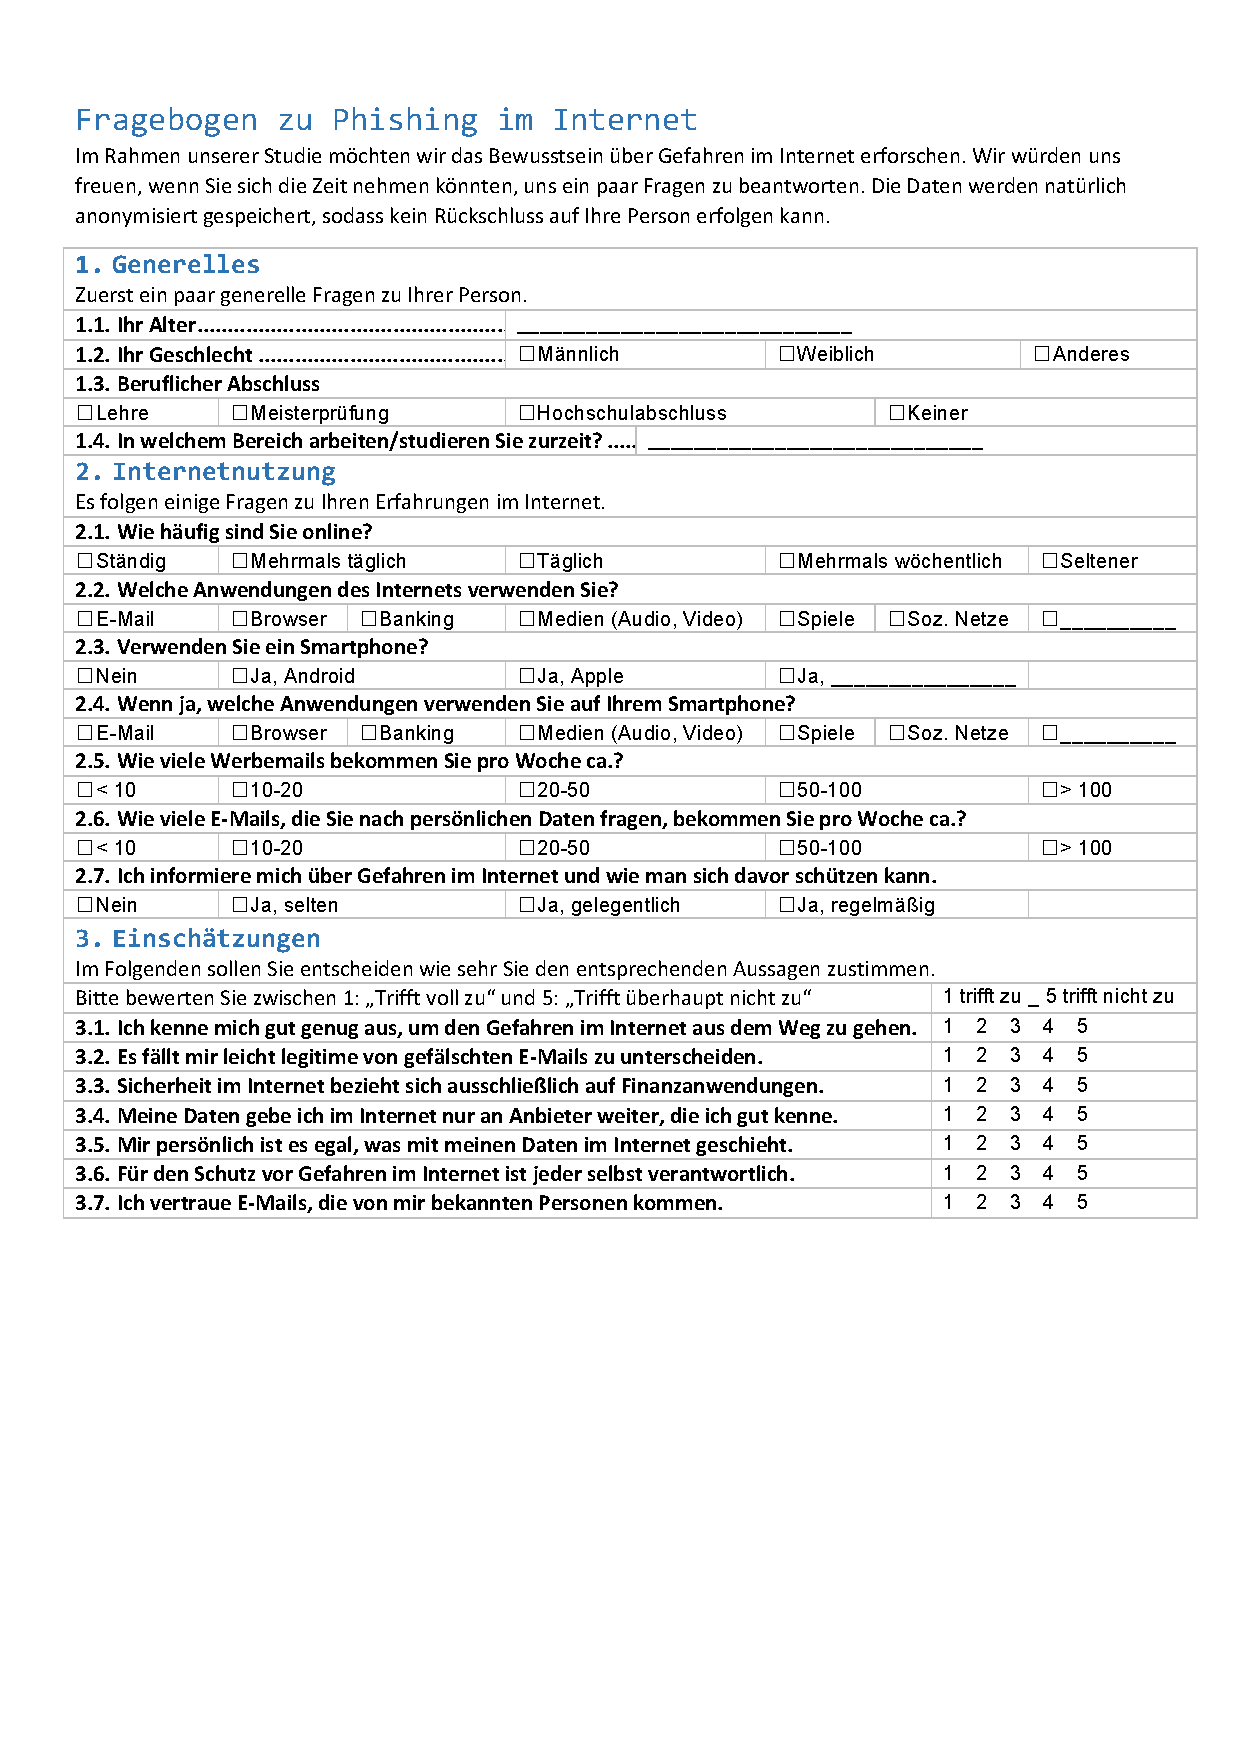
\includepdf[pages=-,frame,scale=0.8]{graphix/presurvey.pdf}


\section{Final Study}

\selectlanguage{ngerman}
\subsection{Participant Recruitment}
\label{s:participant_recruitment_texts}

Sehr geehrte/r ....,
\newline
\newline
wir, Clemens Bergmann und Gamze Canova, sind Studenten des Fachbereichs Informatik an der TU Darmstadt und arbeiten zur Zeit unserer Masterthesis zum Thema Internetsicherheit.
\newline
\newline
Nun sind wir an dem Punkt angekommen, an dem wir eine Benutzerstudie (6.1.-11.1.2014) durchf\"{u}hren m\"{u}ssen, f\"{u}r die wir Teilnehmer suchen. Wir w\"{u}rden uns sehr freuen, wenn Sie uns hierbei unterst\"{u}tzen k\"{o}nnten. W\"{a}re es m\"{o}glich, den angeh\"{a}ngten Flyer mit dem unten stehenden Anschreiben, an Ihre StudentInnen und/oder Wissenschaftliche MitarbeiterInnen  weiterzuleiten? Wir wissen, dass es schwierig sein k\"{o}nnte potentielle Teilnehmer kurz vor Weihnachten zu erreichen, jedoch k\"{o}nnen wir jede Unterst\"{u}tzung gebrauchen und w\"{u}rden uns \"{u}ber diese sehr freuen.
\newline
\newline
Wir bedanken uns im Voraus herzlich f\"{u}r Ihre Bem\"{u}hungen und w\"{u}nschen Ihnen erholsame und besinnliche Festtage.
\newline
\newline
Mit freundlichen Gr\"{u}{\ss}en, \newline
Clemens Bergmann und Gamze Canova
\newline
\newline
Text f\"{u}r Weiterleitung:
Im Rahmen unserer Masterarbeit haben wir eine Spiele-App entwickelt, die fachfremde Benutzer \"{u}ber Internetsicherheit informiert.  Diese App soll im Rahmen einer Benutzerstudie getestet werden. Hierzu brauchen wir deine Hilfe. Die Studie wird in Gruppen zu ca. 5 Personen in der zweiten Januarwoche (6.-10.) in Darmstadt stattfinden und insgesamt ca. 90 Minuten in Anspruch nehmen.  Der/Die Beste der Gruppe gewinnt einen Amazon-Gutschein im Wert von 20\euro.  Einzige Voraussetzung f\"{u}r die Teilnahme ist, dass du Erfahrung mit der Benutzung eines Smartphones hast. Bei Interesse oder Fragen erreicht ihr uns unter netstudy@cased.de. 

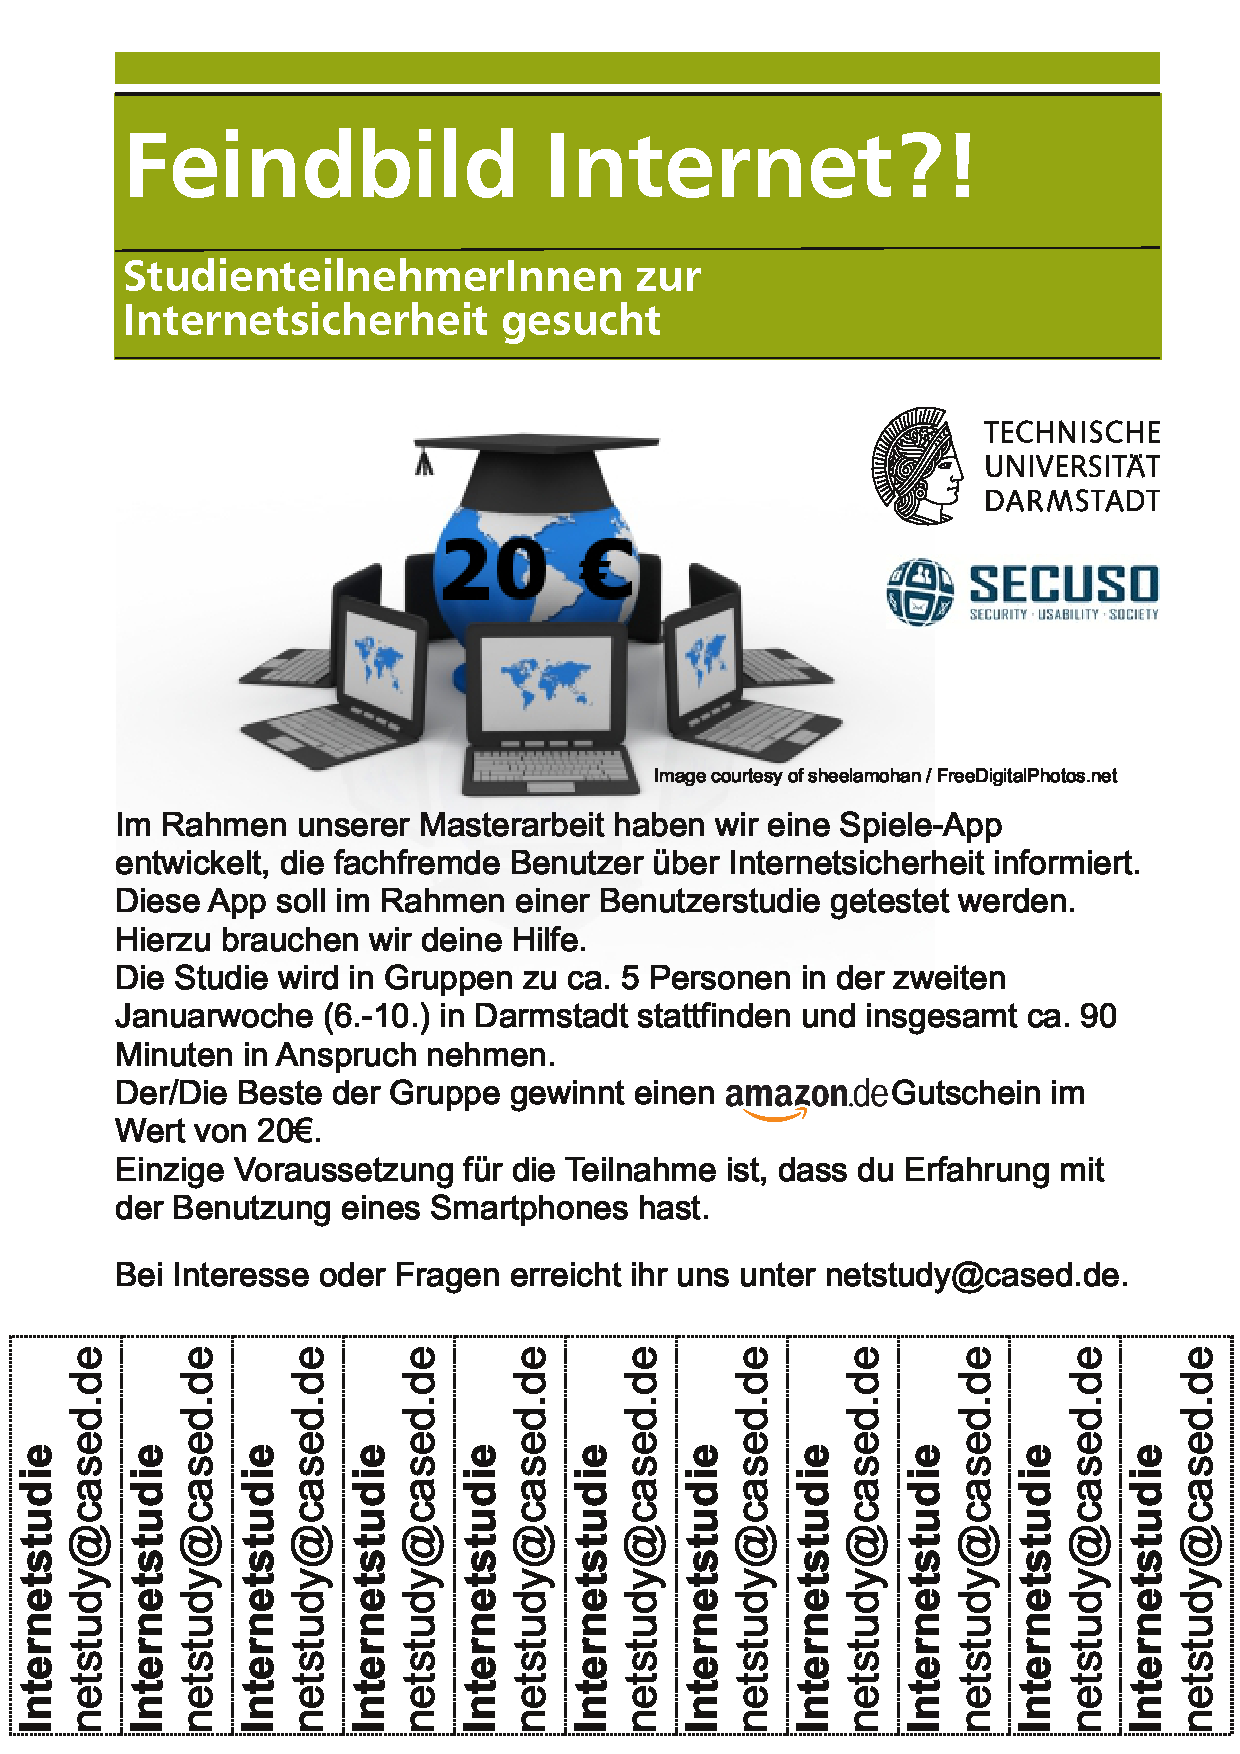
\includepdf[pages={1},frame,scale=0.8]{graphix/flyer.pdf}


\subsection{Explanatory Texts of Each Study Step}
\selectlanguage{american}
In order to ensure that the studies of small groups remain comparable we read all explanatory texts to the participants. 
This section provides a collection of these texts
\selectlanguage{ngerman}

\subsubsection{Welcome and Introduction to Consent Form and General-Survey Before}
Herzlich willkommen zu unserer Benutzerstudie.
Danke, dass ihr euch die Zeit genommen habt uns zu unterst{\"u}tzen.
Bitte bedient euch an den S{\"u}{\ss}igkeiten und dem Wasser auf den Tischen.
W{\"a}hrend der Studie werden wir die Erl{\"a}uterungen vorlesen. Damit wollen wir sicherstellen, dass alle Durchl{\"a}ufe vergleichbar bleiben. 
\newline
\newline
Wir w{\"u}rden euch gerne fragen, ob es in Ordnung f{\"u}r euch w{\"a}re, wenn wir das Gewinnspiel ein bisschen ab{\"a}ndern: wir haben n{\"a}mlich festgestellt, dass es in der Studie in Ausnahmef{\"a}llen passieren kann, dass ihr nicht die gleichen Chancen habt zu gewinnen. Daher w{\"u}rden wir am Ende den Amazon-Gutschein gerne verlosen. Ist das f{\"u}r alle in Ordnung?
Alles klar, super. Dann kanns weiter gehen.
\newline
\newline
In der Studie soll eine App getestet werden, die in Form eines Spiels Benutzern beibringen soll, wie sie sich besser vor Betrug im Internet sch{\"u}tzen k{\"o}nnen. Um das Ganze ein bisschen spannend zu gestalten, wird am Ende die Person ermittelt, die hierbei am besten abgeschnitten hat.
Ziel der Studie ist, die Wirksamkeit der App zu Testen. Hierzu haben wir folgenden Ablauf geplant:
Keine Angst, ihr m{\"u}sst euch nicht die einzelnen Schritte merken, wir erkl{\"a}ren jedes mal was als n{\"a}chstes kommt.
\newline
\newline
Als erstes bekommt ihr zwei Frageb{\"o}gen ausgeteilt.
Der Erste ist eine Einverst{\"a}ndniserkl{\"a}rung, die ihr unterschreiben m{\"u}sst, wenn ihr mitmachen wollt. Auf dem zweiten wird eure Selbsteinsch{\"a}tzung bzgl. eures Wissens zur Internetsicherheit abgefragt.
Im zweiten Teil werden wir an Hand von Beispielen euer Vorwissen zum Thema Internetsicherheit genauer erfassen. Dies dient uns als Basiswert. 
Im dritten Teil werden wir euch Smartphones mit der App austeilen und ihr habt Zeit die App auszuprobieren. 
Dabei sammelt ihr bei dem Spiel Punkte, welche dar{\"u}ber entscheiden, wer von euch vieren das Spiel gewinnt. Dies wird die l{\"a}ngste Zeit in Anspruch nehmen.
Im vierten Teil werden wir euch erneut Beispiele zeigen, um zu erfassen,
in wie weit, die App euch unterst{\"u}tzt. 
Im f{\"u}nften Teil folgt eine "Freispielphase" in der ihr weitere Erfahrungen mit der App sammeln k{\"o}nnt.
Im sechsten Teil folgt ein weitere Fragebogen zur allgemeinen Benutzbarkeit der App.
Anschlie{\ss}end wird der Gewinner ermittelt und (der Amazon-Gutschein verlost) und damit ist die Studie auch beendet. Zuletzt w{\"u}rden wir uns freuen, wenn ihr noch einige Minuten f{\"u}r eine kurze offene Diskussionsrunde bleiben w{\"u}rdet, um eure Anmerkungen loszuwerden.
Soviel zum Ablauf.
\newline
\newline
Bei Fragen oder Problemen mit der App meldet euch einfach und wir kommen zu euch um die anderen nicht unn{\"o}tig zu st{\"o}ren. Wir werden euch bei technischen Problemen oder Bedienungsproblemen helfen. Inhaltliche Fragen k{\"o}nnen wir nicht beantworten weil dadurch der Einfluss der App auf euch nicht mehr gepr{\"u}ft werden k{\"o}nnte.
Ihr habt jederzeit das Recht zu gehen und die Studie abzubrechen. Beachtet aber: Wenn ihr die Studie nicht vollst{\"a}ndig mitmacht, k{\"o}nnt ihr nat{\"u}rlich nicht am Gewinnspiel teilnehmen.
\newline
\newline
Wichtig ist: Bitte bearbeitet alle Fragen und die App alleine. Ihr k{\"o}nnt nichts falsch machen. Beantwortet einfach alle Fragen nach besten wissen. Damit helft ihr uns am meisten. Wenn ihr mit dem Ausf{\"u}llen jeweils fertig seid gebt uns die Frageb{\"o}gen einfach zur{\"u}ck.
Habt ihr dazu noch Fragen?
\newline
\newline
Bevor es jetzt losgeht, wollten wir noch darauf hinweisen, dass die Studie ab jetzt ca. 1 Stunde dauern wird. Wegen des Studienaufbaus ist es leider nicht m{\"o}glich sie zwischendurch kurz zu unterbrechen, daher nutzt jetzt bitte die Gelegenheit, falls ihr kurz raus m{\"u}sst.
\newline
\newline
Ok, bevor es losgeht w{\"u}rden wir euch gerne darum bitten, eure Handys auf lautlos zu schalten und auch die Vibration auszustellen. Danke.
Hier sind erst einmal die Einverst{\"a}ndniserkl{\"a}rungen. Wenn ihr damit fertig seid, geben wir euch den zweiten Fragebogen.

\subsubsection{Introduction to Website-Survey Before}
Nachdem wir nun wissen was ihr vor dieser Studie {\"u}ber Internetsicherheit wusstet, k{\"o}nnen wir nun etwas konkreter werden.
Bei der App handelt es sich um ein Spiel welches euch speziell Tips zum Thema Phishing gibt.
Phishing ist ein Betrugsversuch. Hierbei spielt der Betr{\"u}ger dem Benutzer vor jemand anderes zu sein. Das Ziel des Betr{\"u}gers ist, dem Benutzer pers{\"o}nliche Informationen zu entlocken. Meistens macht er das {\"u}ber gef{\"a}lschte Webseiten.
\newline
\newline
Im n{\"a}chsten Fragebogen zeigen wir euch daher ein paar Webseiten. Ihr m{\"u}sst entscheiden, ob diese gef{\"a}lscht oder legitim sind.
F{\"u}r unsere Auswertung ist es wichtig, dass ihr die Seiten in der vorgegebenen Reihenfolge beantwortet und nicht zur{\"u}ck bl{\"a}ttert, auch wenn euch im Nachhinein etwas auff{\"a}llt. Schaut lieber zweimal hin.

\subsubsection{Introduction to Playing App}
So, jetzt ist die App an der Reihe.
Wir teilen euch jetzt die Smartphones aus.
Zus{\"a}tzlich teilen wir euch einen Zettel aus. Darauf k{\"o}nnt ihr Anmerkungen zur App direkt notieren.
Diesen k{\"o}nnt ihr bis zum Ende behalten und weiterhin Notizen darauf machen. Ihr k{\"o}nnt ihn dann am Ende mit dem letzen Fragebogen abgeben.
\newline
\newline
Jedes Telefon ist mit der Nummer eures Sitzplatzes beschriftet. Bitte verwendet nur euer Telefon.
Auf dem Starbildschirm der Handys befindet sich die App. Sie hei{\ss}t ``NoPhish''.
Wenn wir euch sagen, dass es losgeht, startet die App durch Antippen und w{\"a}hlt im Startmen{\"u} auf den gr{\"u}nen Button, um das Spiel zu starten.
Ihr habt zum Spielen 30 Minuten zeit.
\newline
\newline
Im Laufe der App, werdet ihr nach eurer E-Mail Adresse gefragt. Dazu sind auf den Smartphones speziell f{\"u}r die Studie E-Mail Adressen angelegt worden. Diese werden euch bei der Eingabe in das Feld vorgeschlagen. Bitte w{\"a}hlt diese aus. Bei der Absender-Adresse d{\"u}rft ihr eingeben, was ihr wollt.
\newline
\newline
Es ist nicht m{\"o}glich die App in der Zeit vollst{\"a}ndig durchzuspielen. Spielt einfach so weit ihr kommt.
Wenn wir euch am Ende bescheid geben h{\"o}rt bitte einfach auf die App zu spielen und lasst sie so wie sie ist. Nur so k{\"o}nnen wir eure Punktzahl korrekt ablesen.
Jetzt geht's los. Viel erfolg.


\subsubsection{Introduction to Website-Survey After and Further App Exploration}
Die Zeit ist um. Bitte legt jetzt die Smartphones weg. Wir sammeln sie jetzt ein.
\newline
\newline
Jetz kommt nochmal ein Fragebogen mit Webseiten. Wie vorher sollt ihr darauf entscheiden ob eine Webseite gef{\"a}lscht oder legitim ist. Wenn ihr damit fertig seid gebt den Fragebogen uns wieder zur{\"u}ck.
\newline
\newline
Jetzt teilen wir wieder die Smartphones aus. Wir bitten euch diesmal die anderen Funktionen der App auszutesten. Daf{\"u}r habt ihr dann nochmal 5 Minuten.


\subsubsection{Introduction to General-Survey After}
Zum Schluss nochmal ein Fragebogen zur Benutzbarkeit. Wenn ihr damit fertig seid, gebt ihn bitte zusammen mit eurem Notizzettel wieder ab.

\subsubsection{Issuance of Certificates, Debrief and Goodbye}
Ihr habt es geschafft.
Vielen Dank, dass ihr euch die Zeit genommen habt, die App zu testen.
Haben sich bei euch noch Fragen ergeben?
\newline
\newline
Alles klar, dann kommen wir zur Bekanntgabe des Gewinners vom Spiel.
Gewonnen hat <gewinnername/>, mit <gewinnerpunkte/> Punkten.
Herzlichen Gl{\"u}ckwunsch, du hast am besten abgeschnitten. 
\newline
\newline
Nun kommen wir zur Verlosung des Amazon-Gutscheins. 
<name/> hat den Amazon-Gutschein gewonnen, herzlichen Gl{\"u}ckwunsch. \newline
<Erhaltbest{\"a}tigung unterschreiben lassen/>
\newline
\newline
Allen anderen vielen Dank nochmal f{\"u}r eure Teilnahme.\newline
<Austeilen der Anti-Phishing Awards>
\newline
\newline
Zum Schluss w{\"u}rden wir uns freuen, wenn ihr noch in einer kurzen Diskussionsrunde mitmachen w{\"u}rdet. Diese ist freiwillig. Wer m{\"o}chte jetzt gerne gehen? Sehr sch{\"o}n, danke.
\newline
\newline
Die offene Diskussion w{\"u}rden wir gerne mit einem Diktierger{\"a}t aufzeichnen. Ist das f{\"u}r alle in Ordnung?
\newline
\newline
Nochmal vielen Dank an alle Teilnehmer.
Wir hoffen es hat euch etwas Spa{\ss} gemacht und w{\"u}nschen euch noch einen sch{\"o}nen Tag.
Nehmt euch gerne noch Kekse und Gummib{\"a}rchen f{\"u}r auf den Weg mit.
\newline
\newline
Tsch{\"u}ss
\selectlanguage{american}

\subsection{Study Forms}
The following pages contain the forms as we used them in the user study. We did not include all example URL but only one exemplary page with an attacked URL.
\label{s:before_survey}
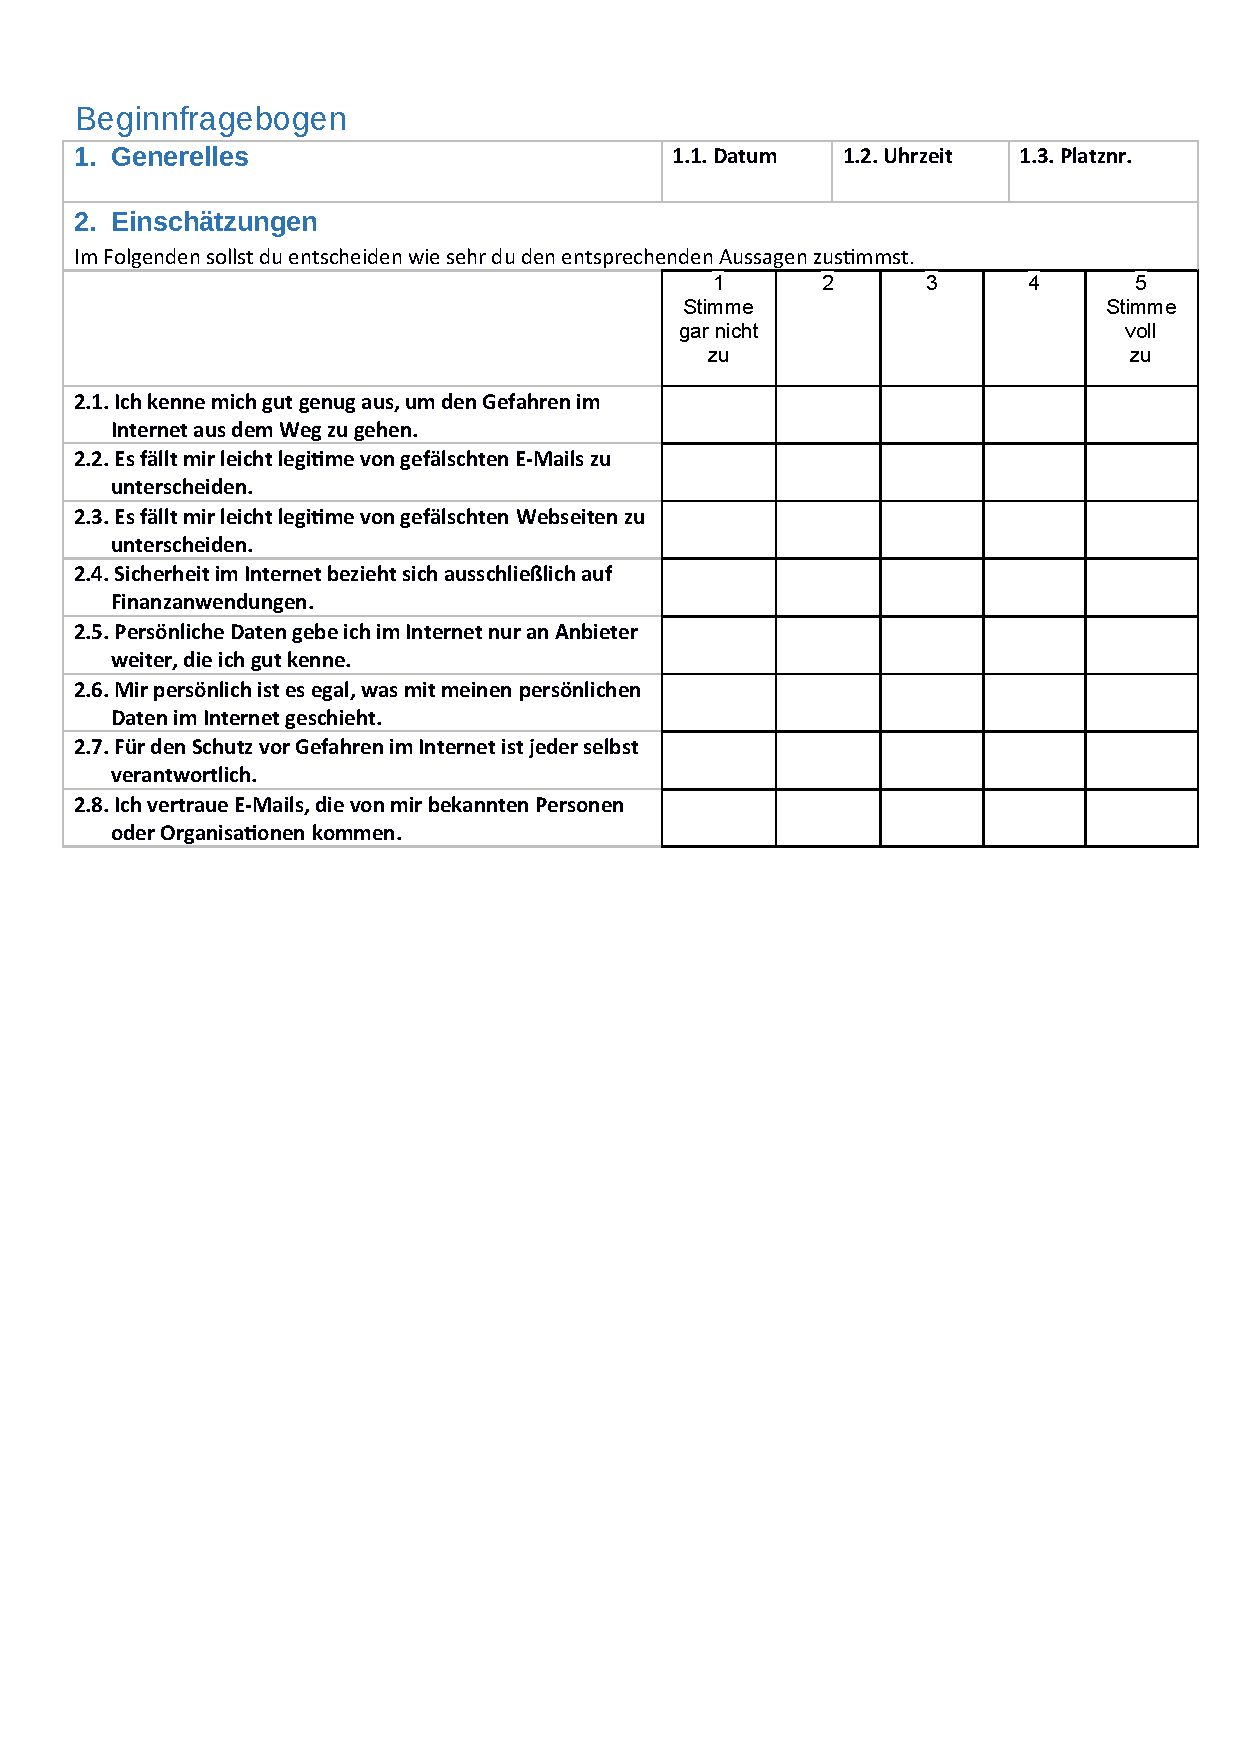
\includepdf[pages=-,frame,scale=0.8]{graphix/before_survey.pdf}
\label{s:url_survey}
\includepdf[pages={1,10},frame,scale=0.8]{graphix/url_survey.pdf}
\label{s:after_survey}
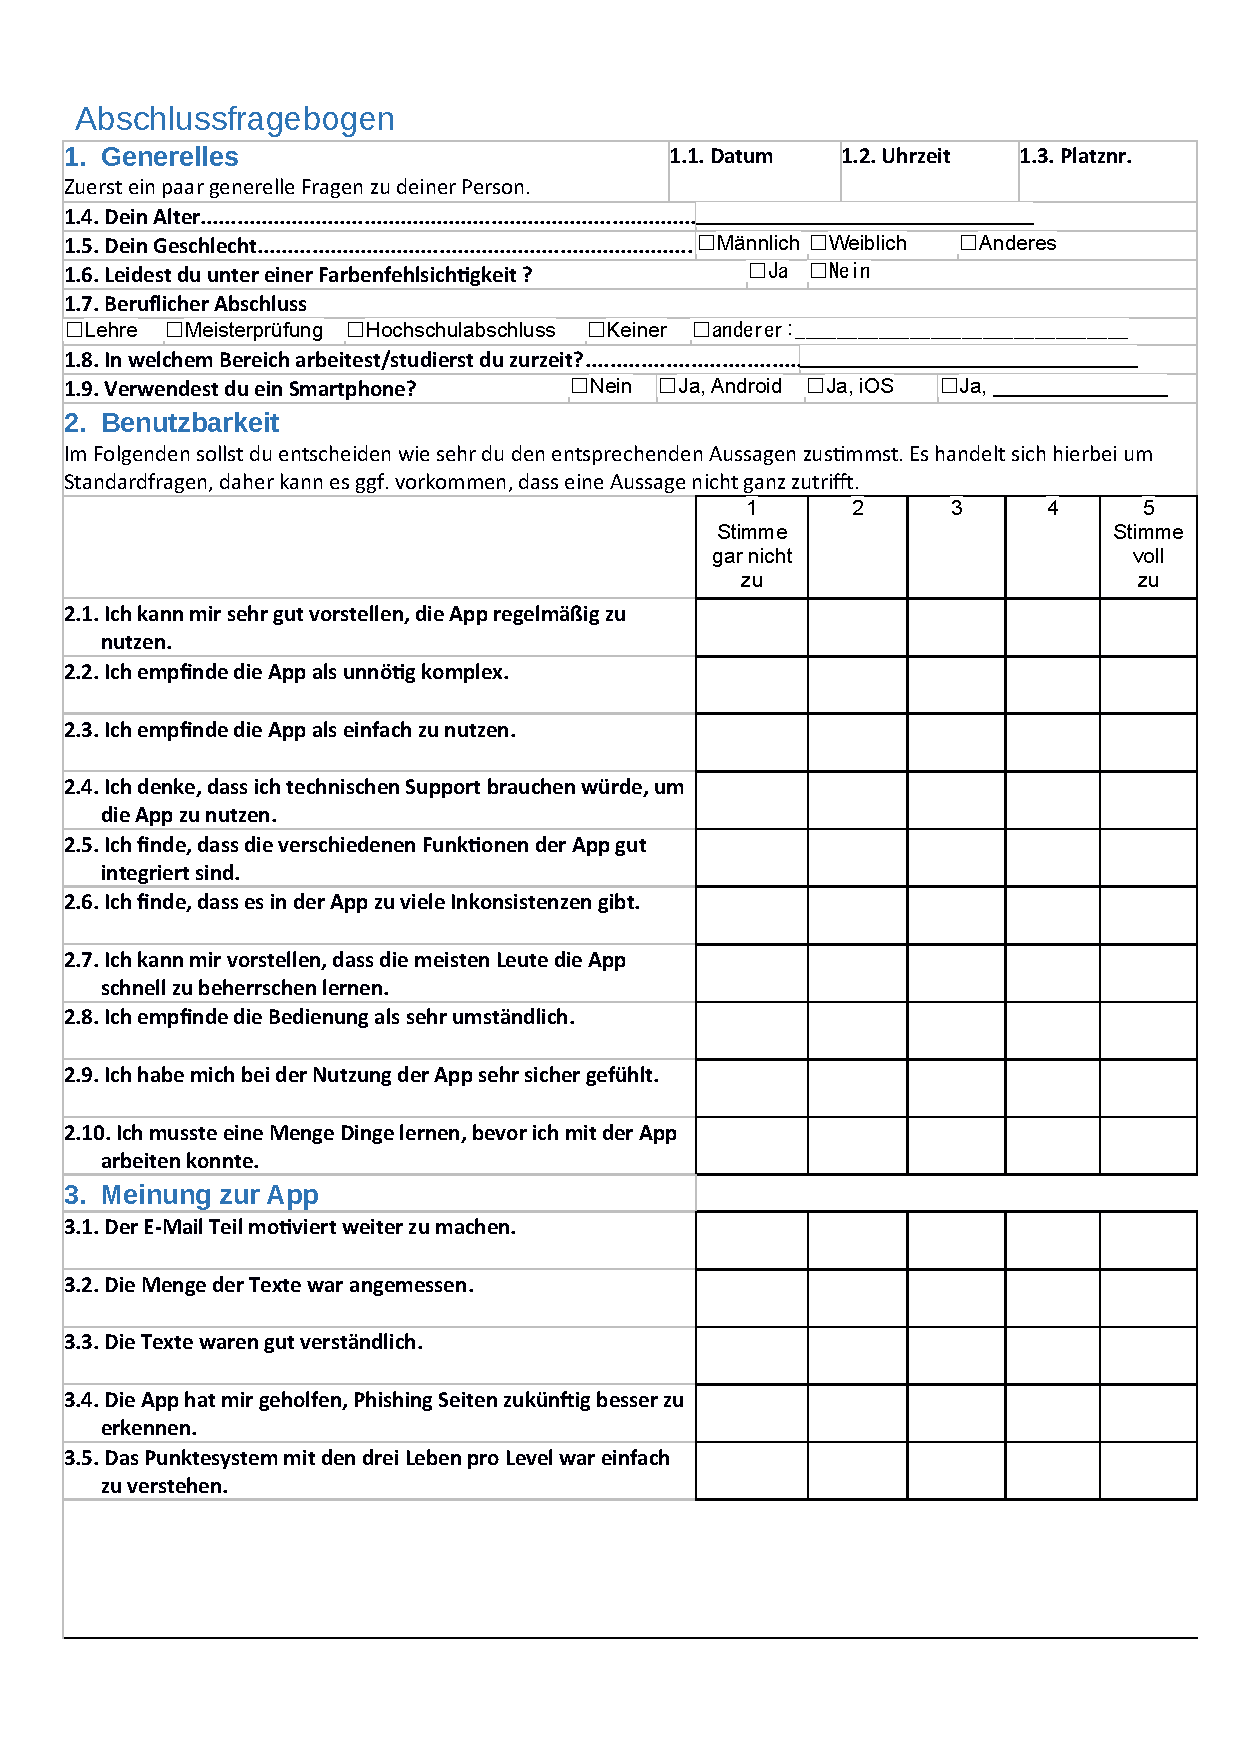
\includepdf[pages={1},frame,scale=0.8]{graphix/after_survey.pdf}

\subsubsection{Example URLs of Website-Survey Before}
\label{example_urls_before}
\begin{enumerate}
\item \url{https://plus.google.com/u/0/me}
\item \url{https://www.facebook.signin.com/Raumzeit}
\item \url{http://m.youtube.com/watch?v=Ctzc8QSF6mQ}
\item \url{http://www.amazon.de/Angebote/b/ref=cs_top_nav_gb27?ie=UTF8&}
\item \url{http://130.83.162.6/wiki/Wikipedia:Hauptseite}
\item \url{http://www.ebay.de/rpp/Deals/reisen-gutscheine/stadte-kultur/}
\item \url{https://web.de.myponyfarm.com/}
\item \url{http://abo.net/www.focus.de/digital/}
\item \url{http://www.gmx.net/produkte/mail/promail/}
\item \url{http://de.yahoo.com/?p=us}
\item \url{https://www.ott0.de/damenmode/kategorien/anzuege-kostueme}
\item \url{http://windows.mircosoft.com/de-de/windows/products}
\item \url{http://badcat.com/mobile.twitter.com/session/new}
\item \url{https://touch.www.linkedin.com/login.html}
\item \url{http://m.spiegel.de/panorama/leute/a-937125.html#spRedir}
\item \url{https://www.paypal-sicher.com/webapps/merchantboarding/web}
\end{enumerate}


\subsubsection{Example URLs of Website-Survey After}
\label{example_urls_after}

\begin{enumerate}
\item \url{http://www.amazon.de/Angebote/b/ref=cs_top_nav_gb27?ie=UTF8&}
\item \url{http://www.gutefrage.net.events-ma.de/tag/freizeit/1}
\item \url{http://www.t-online.de/wetter/europawetter/64077226}
\item \url{http://www.immobilienscout25.de/de/finden/wohnen/index.jsp}
\item \url{http://www.ebay.de/rpp/Deals/reisen-gutscheine/stadte-kultur/}
\item \url{http://de.yahoo.com/?p=us}
\item \url{https://130.83.162.6/signup/}
\item \url{https://plus.google.com/u/0/me}
\item \url{http://abo.net/www.focus.de/digital/}
\item \url{http://epaper.bild.de/}
\item \url{https://www.facebook.signin.com/Raumzeit}
\item \url{http://www.welt.de/sonderthemen/mittelstand/forschung/}
\item \url{https://web.de.myponyfarm.com/}
\item \url{http://windows.mircosoft.com/de-de/windows/products}
\item \url{http://www.gmx.net/produkte/mail/promail/}
\item \url{https://mail.live.dub123.com/login.srf?wa=wsignin1.0&rpsnv=12}
\item \url{http://m.youtube.com/watch?v=Ctzc8QSF6mQ}
\item \url{https://www.ott0.de/damenmode/kategorien/anzuege-kostueme/}
\item \url{http://130.83.162.6/wiki/Wikipedia:Hauptseite}
\item \url{https://www.paypal-sicher.com/webapps/merchantboarding/web}
\item \url{https://touch.www.linkedin.com/login.html}
\item \url{http://m.spiegel.de/panorama/leute/a-937125.html#spRedire}
\item \url{http://badcat.com/mobile.twitter.com/session/new}
\item \url{https://blog.xing.com/category/german/}
\end{enumerate}


\subsection{Anti-Phish Certificates for Study Participants}
\label{s:antiphish_certs}

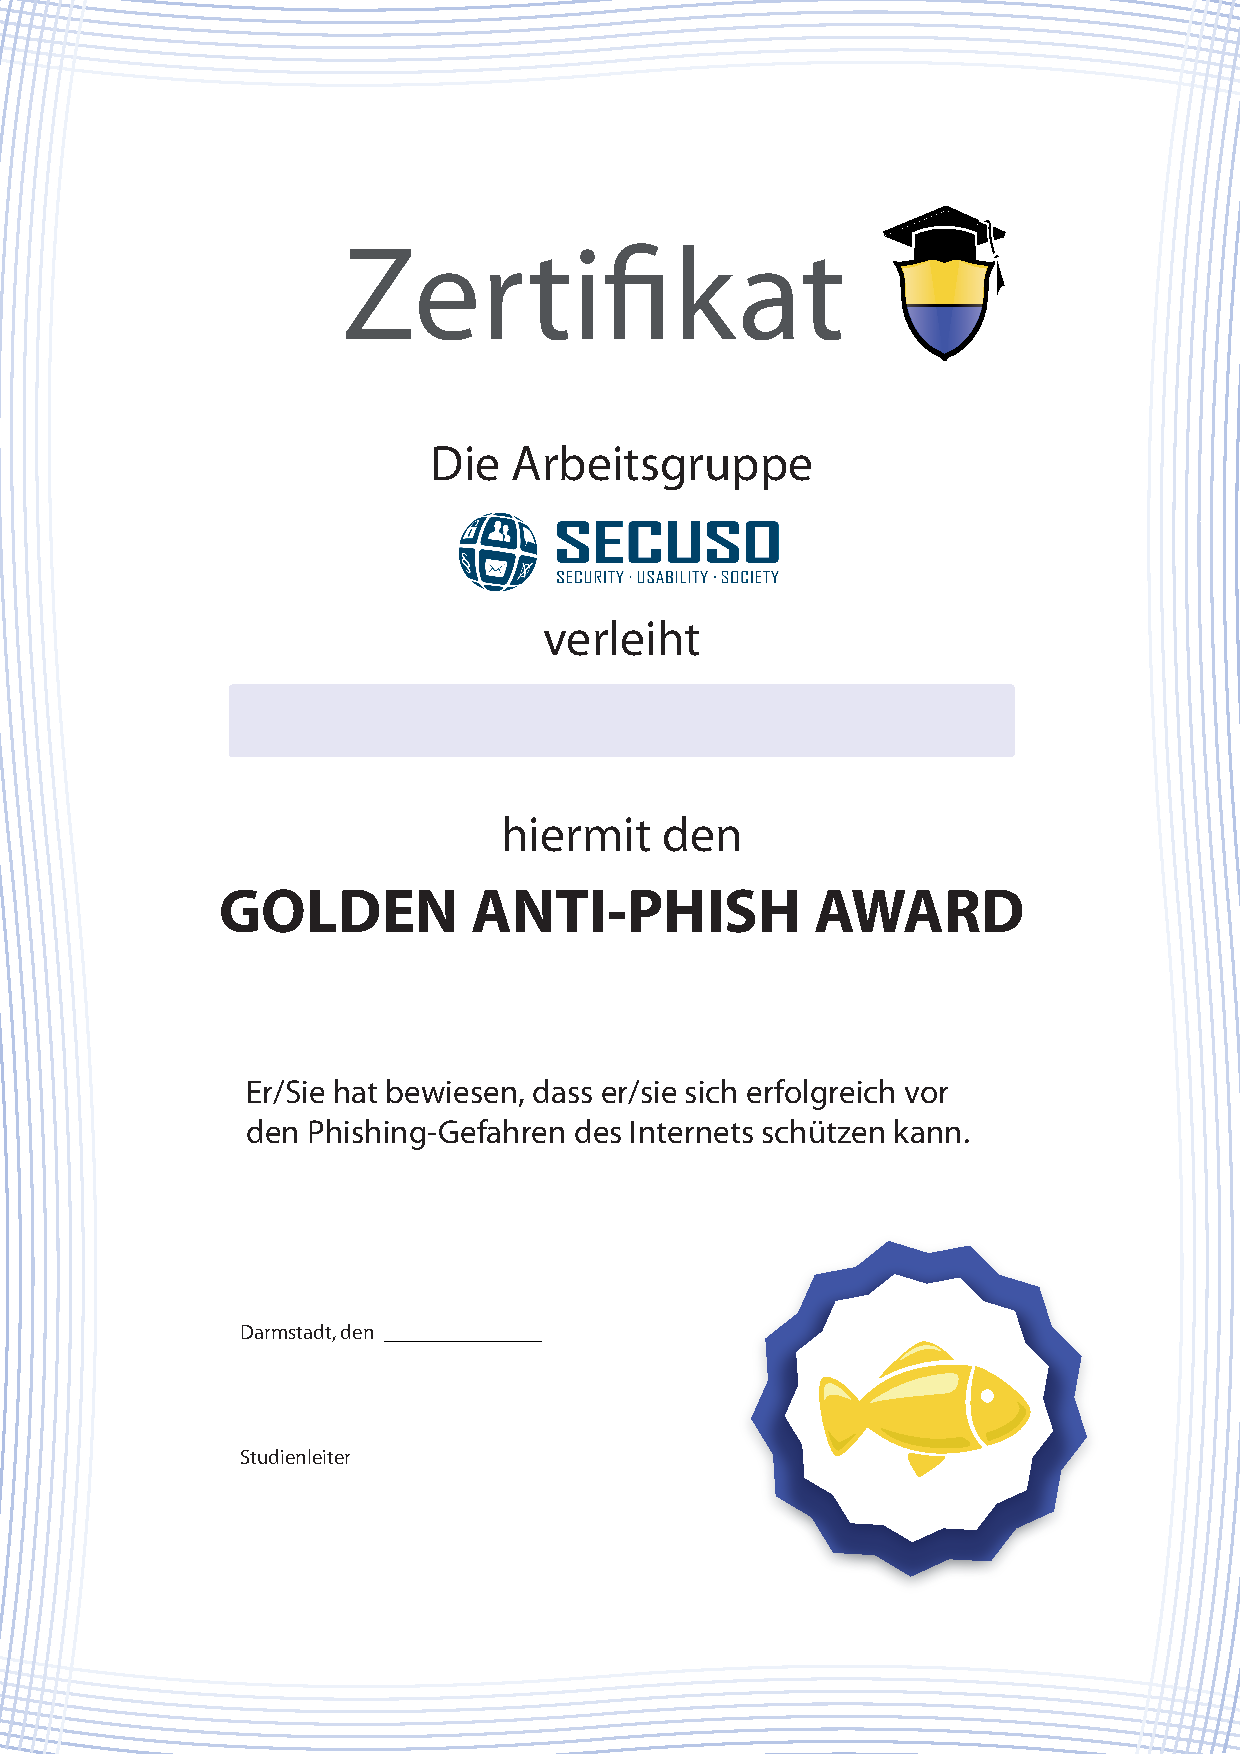
\includepdf[pages={1},frame,scale=0.8]{graphix/zertifikat_gold.pdf}
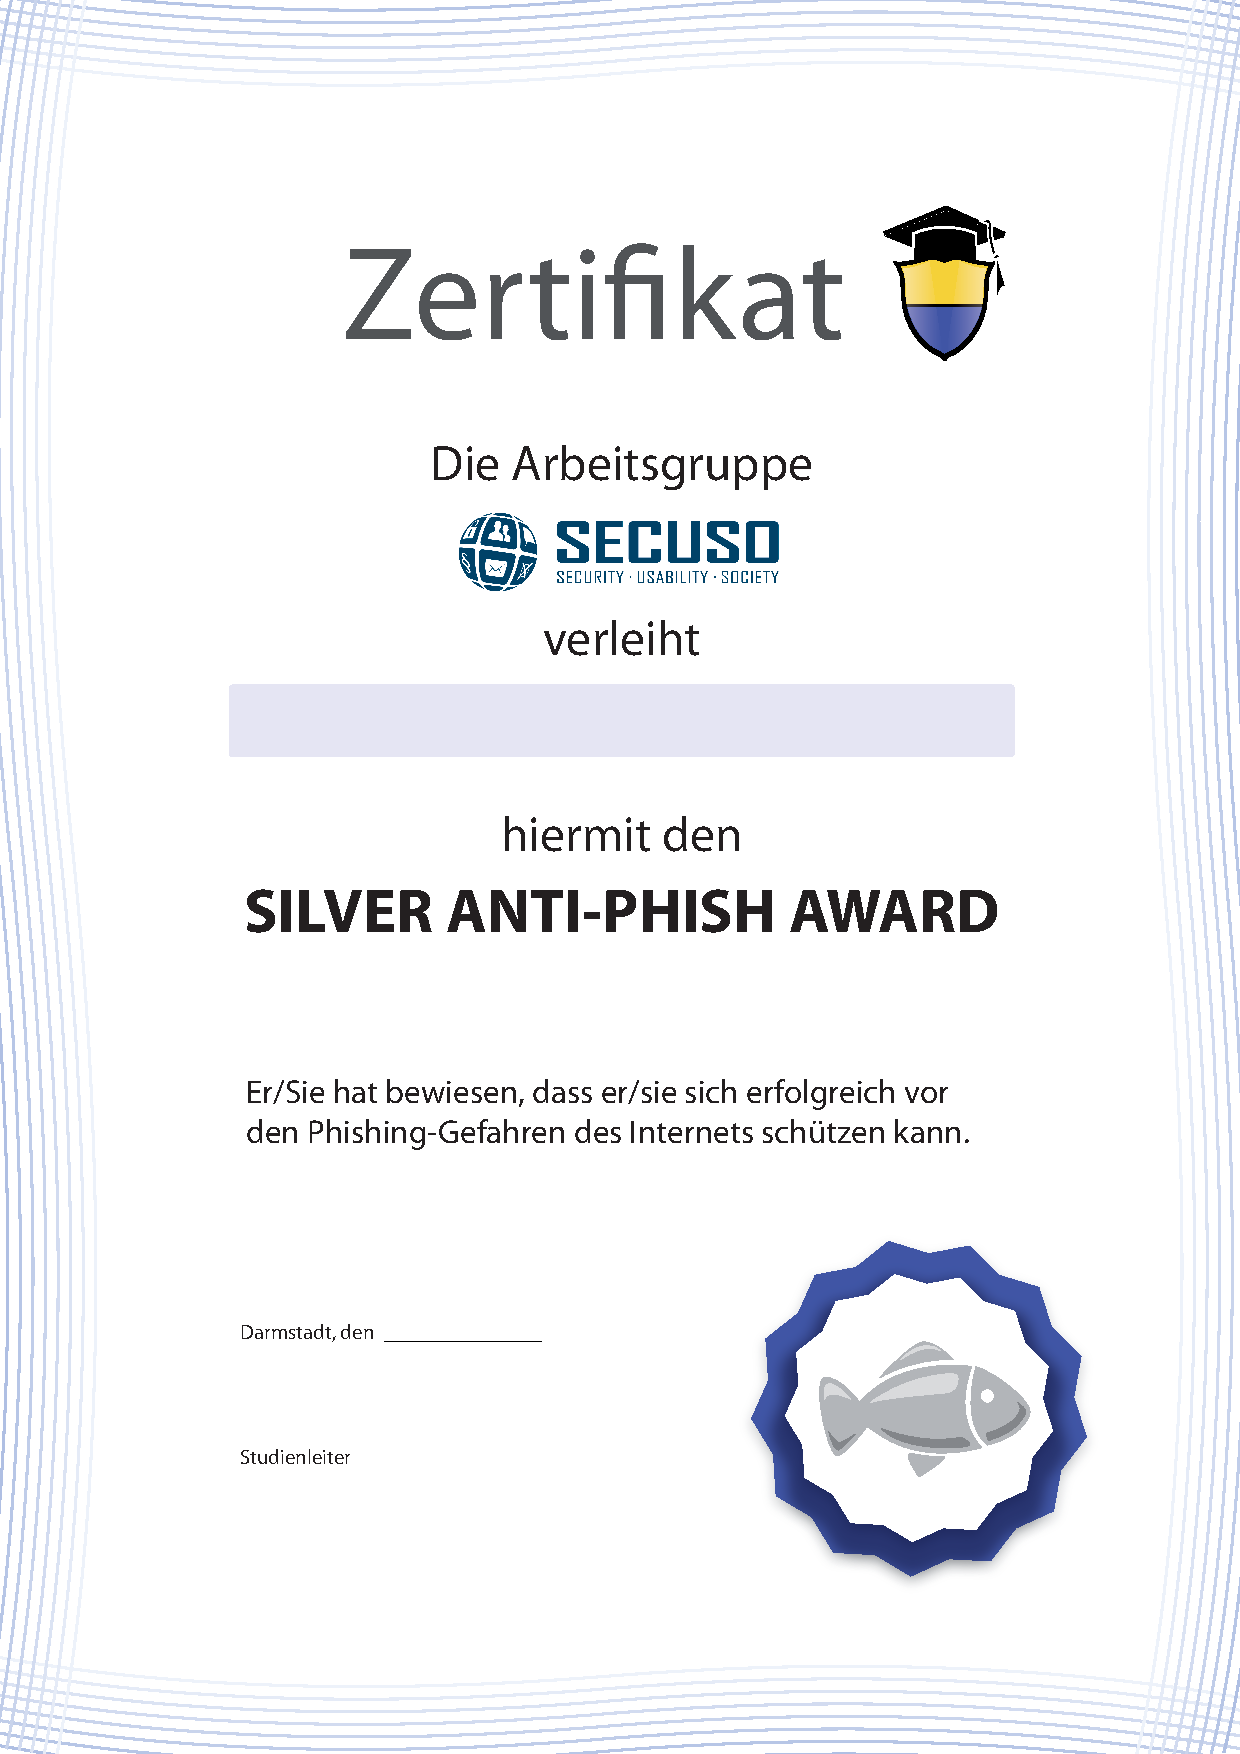
\includepdf[pages={1},frame,scale=0.8]{graphix/zertifikat_silber.pdf}

\section{Thesis contributions}
We (Gamze Canova and Clemens Bergmann) worked on this thesis together.
Therefore we list in the following sections who wrote what part of the thesis and what we did together.

\subsection*{Together}
\begin{tabular}{ll}
\Cref{s:introduction}&"\nameref{s:introduction}"\\
\Cref{s:evaluation}&"\nameref{s:evaluation}"\\
\Cref{s:conclusion}&"\nameref{s:conclusion}"
\end{tabular}

\subsection*{Gamze Canova}
\begin{tabular}{ll}
\Cref{s:related_work}&"\nameref{s:related_work}"\\
\Cref{s:focus}&"\nameref{s:focus}"\\
\Cref{s:survey}&"\nameref{s:survey}"\\
\Cref{s:knowledgetransferperlevel}&"\nameref{s:knowledgetransferperlevel}"\\
\Cref{s:leveling}&"\nameref{s:leveling}"\\
\Cref{s:learning_principles_and_game_techniques}&"\nameref{s:learning_principles_and_game_techniques}"\\
\Cref{s:mockup}&"\nameref{s:mockup}"\\
\Cref{s:pilot_study}&"\nameref{s:pilot_study}"\\
\end{tabular}

\subsection*{Clemens Bergmann}

\begin{tabular}{ll}
\Cref{s:background}&"\nameref{s:background}"\\
\Cref{s:target_group}&"\nameref{s:target_group}"\\
\Cref{s:app_teaching_content}&"\nameref{s:app_teaching_content}"\\
\Cref{s:app_design}&"\nameref{s:app_design}"\\
\Cref{s:gamafication}&"\nameref{s:gamafication}"\\
\Cref{s:game_rules}&"\nameref{s:game_rules}"\\
\Cref{s:legibility_index}&"\nameref{s:legibility_index}"\\
\Cref{s:implementation_testing}&"\nameref{s:implementation_testing}"\\
\end{tabular}

	\end{appendix}
	
	\bibliographystyle{abbrv} % <--- layout of the bib
	\bibliography{bibliography} % file name of your bib

\end{document}
